\documentclass{article}

% if you need to pass options to natbib, use, e.g.:
%     \PassOptionsToPackage{numbers, compress}{natbib}
% before loading neurips_2021
\usepackage[numbers,sort&compress]{natbib}
%\usepackage[natbib]{neurips_2021}

\usepackage{microtype}
\usepackage{graphicx}
\usepackage{subfigure}
\usepackage{booktabs} % for professional tables
\usepackage{textcomp}

% ready for submission
\usepackage[final]{neurips_2021}
\usepackage{color}
\usepackage{multirow}
\usepackage{bbm}
\usepackage{bm}
\usepackage{amsfonts,amssymb}
\usepackage{amsmath}
\usepackage{graphicx} %use graph format
\usepackage{epstopdf}

\usepackage[all]{xy}
\usepackage{amsmath}
\usepackage{wrapfig}
% to compile a preprint version, e.g., for submission to arXiv, add add the
% [preprint] option:
%     \usepackage[preprint]{neurips_2021}

% to compile a camera-ready version, add the [final] option, e.g.:
% \usepackage[final]{neurips_2021}

% to avoid loading the natbib package, add option nonatbib:
%    \usepackage[nonatbib]{neurips_2021}


% Attempt to make hyperref and algorithmic work together better:
\newcommand{\tabincell}[2]{\begin{tabular}{@{}#1@{}}#2\end{tabular}}

\newcommand{\theHalgorithm}{\arabic{algorithm}}

\usepackage{algorithmic}
\usepackage{algorithm}
\usepackage{amsmath}
\usepackage[utf8]{inputenc} % allow utf-8 input
\usepackage[T1]{fontenc}    % use 8-bit T1 fonts
\usepackage{hyperref}       % hyperlinks
\usepackage{url}            % simple URL typesetting
\usepackage{booktabs}       % professional-quality tables
\usepackage{amsfonts}       % blackboard math symbols
\usepackage{nicefrac}       % compact symbols for 1/2, etc.
\usepackage{microtype}      % microtypography
\usepackage{xcolor}         % colors
\usepackage{stfloats}

\newcommand{\Amat}[0]{\ensuremath{{\bf A}}}
\newcommand{\Bmat}[0]{\ensuremath{{\bf B}} }
\newcommand{\Cmat}[0]{\ensuremath{{\bf C}} }
\newcommand{\Dmat}[0]{\ensuremath{{\bf D}} }
\newcommand{\Emat}[0]{\ensuremath{{\bf E}} }
\newcommand{\Fmat}[0]{\ensuremath{{\bf F}} }
\newcommand{\Gmat}[0]{\ensuremath{{\bf G}} }
\newcommand{\Hmat}[0]{\ensuremath{{\bf H}} }
\newcommand{\Imat}[0]{\ensuremath{{\bf I}} }
\newcommand{\Jmat}[0]{\ensuremath{{\bf J}} }
\newcommand{\Kmat}[0]{\ensuremath{{\bf K}} }
\newcommand{\Lmat}[0]{\ensuremath{{\bf L}} }
\newcommand{\Mmat}[0]{\ensuremath{{\bf M}} }
\newcommand{\Nmat}[0]{\ensuremath{{\bf N}} }
\newcommand{\Omat}[0]{\ensuremath{{\bf O}} }
\newcommand{\Pmat}[0]{\ensuremath{{\bf P}} }
\newcommand{\Qmat}[0]{\ensuremath{{\bf Q}} }
\newcommand{\Rmat}[0]{\ensuremath{{\bf R}} }
\newcommand{\Smat}[0]{\ensuremath{{\bf S}} }
\newcommand{\Tmat}[0]{\ensuremath{{\bf T}} }
\newcommand{\Umat}[0]{\ensuremath{{\bf U}} }
\newcommand{\Vmat}[0]{\ensuremath{{\bf V}} }
\newcommand{\Wmat}[0]{\ensuremath{{\bf W}} }
\newcommand{\Xmat}[0]{\ensuremath{{\bf X}} }
\newcommand{\Ymat}[0]{\ensuremath{{\bf Y}} }
\newcommand{\Zmat}[0]{\ensuremath{{\bf Z}} }

\newcommand{\mc}{\multicolumn}
\newcommand{\mr}{\multirow}
\newcommand{\av}[0]{\ensuremath{\boldsymbol{a}} }
\newcommand{\bv}[0]{\ensuremath{\boldsymbol{b}} }
\newcommand{\cv}[0]{\ensuremath{\boldsymbol{c}} }
\newcommand{\dv}[0]{\ensuremath{\boldsymbol{d}} }
\newcommand{\ev}[0]{\ensuremath{\boldsymbol{e}} }
\newcommand{\fv}[0]{\ensuremath{\boldsymbol{f}} }
\newcommand{\gv}[0]{\ensuremath{\boldsymbol{g}} }
\newcommand{\hv}[0]{\ensuremath{\boldsymbol{h}} }
\newcommand{\iv}[0]{\ensuremath{\boldsymbol{i}} }
\newcommand{\jv}[0]{\ensuremath{\boldsymbol{j}} }
\newcommand{\kv}[0]{\ensuremath{\boldsymbol{k}} }
\newcommand{\lv}[0]{\ensuremath{\boldsymbol{l}} }
\newcommand{\mv}[0]{\ensuremath{\boldsymbol{m}} }
\newcommand{\nv}[0]{\ensuremath{\boldsymbol{n}} }
\newcommand{\ov}[0]{\ensuremath{\boldsymbol{o}} }
\newcommand{\pv}[0]{\ensuremath{\boldsymbol{p}} }
\newcommand{\qv}[0]{\ensuremath{\boldsymbol{q}} }
\newcommand{\rv}[0]{\ensuremath{\boldsymbol{r}} }
\newcommand{\sv}[0]{\ensuremath{\boldsymbol{s}} }
\newcommand{\tv}[0]{\ensuremath{\boldsymbol{t}} }
\newcommand{\uv}[0]{\ensuremath{\boldsymbol{u}} }
\newcommand{\wv}[0]{\ensuremath{\boldsymbol{w}} }
\newcommand{\xv}[0]{\ensuremath{\boldsymbol{x}} }
\newcommand{\yv}[0]{\ensuremath{\boldsymbol{y}} }
\newcommand{\zv}[0]{\ensuremath{\boldsymbol{z}} }
\newcommand{\vv}[0]{\ensuremath{\boldsymbol{v}} }
\newcommand{\Av}[0]{\ensuremath{\boldsymbol{A}} }
\newcommand{\Bv}[0]{\ensuremath{\boldsymbol{B}} }
\newcommand{\Cv}[0]{\ensuremath{\boldsymbol{C}} }
\newcommand{\Dv}[0]{\ensuremath{\boldsymbol{D}} }
\newcommand{\Ev}[0]{\ensuremath{\boldsymbol{E}} }
\newcommand{\Fv}[0]{\ensuremath{\boldsymbol{F}} }
\newcommand{\Gv}[0]{\ensuremath{\boldsymbol{G}} }
\newcommand{\Hv}[0]{\ensuremath{\boldsymbol{H}} }
\newcommand{\Iv}[0]{\ensuremath{\boldsymbol{I}} }
\newcommand{\Jv}[0]{\ensuremath{\boldsymbol{J}} }
\newcommand{\Kv}[0]{\ensuremath{\boldsymbol{K}} }
\newcommand{\Lv}[0]{\ensuremath{\boldsymbol{L}} }
\newcommand{\Mv}[0]{\ensuremath{\boldsymbol{M}} }
\newcommand{\Nv}[0]{\ensuremath{\boldsymbol{N}} }
\newcommand{\Ov}[0]{\ensuremath{\boldsymbol{O}} }
\newcommand{\Pv}[0]{\ensuremath{\boldsymbol{P}} }
\newcommand{\Qv}[0]{\ensuremath{\boldsymbol{Q}} }
\newcommand{\Rv}[0]{\ensuremath{\boldsymbol{R}} }
\newcommand{\Sv}[0]{\ensuremath{\boldsymbol{S}} }
\newcommand{\Tv}[0]{\ensuremath{\boldsymbol{T}} }
\newcommand{\Uv}[0]{\ensuremath{\boldsymbol{U}} }
\newcommand{\Vv}[0]{\ensuremath{\boldsymbol{V}} }
\newcommand{\Wv}[0]{\ensuremath{\boldsymbol{W}} }
\newcommand{\Xv}[0]{\ensuremath{\boldsymbol{X}} }
\newcommand{\Yv}[0]{\ensuremath{\boldsymbol{Y}} }
\newcommand{\Zv}[0]{\ensuremath{\boldsymbol{Z}} }
\newcommand{\piv}[0]{\ensuremath{\boldsymbol{\pi}} }
\newcommand{\Piv}[0]{\ensuremath{\boldsymbol{\Pi}} }
\newcommand{\phiv}[0]{\ensuremath{\boldsymbol{\phi}} }
\newcommand{\Phiv}[0]{\ensuremath{\boldsymbol{\Phi}} }
\newcommand{\betav}[0]{\ensuremath{\boldsymbol{\beta}} }
\newcommand{\thetav}[0]{\ensuremath{\boldsymbol{\theta}} }
\newcommand{\lambdav}[0]{\ensuremath{\boldsymbol{\lambda}} }
\newcommand{\epsilonv}[0]{\ensuremath{\boldsymbol{\epsilon}} }
\newcommand{\Omegav}[0]{\ensuremath{\boldsymbol{\Omega}} }
\newcommand{\etav}[0]{\ensuremath{\boldsymbol{\eta}} }
\newcommand{\Sigmav}[0]{\ensuremath{\boldsymbol{\Sigma}}}
\newcommand{\Lambdav}[0]{\ensuremath{\boldsymbol{\Lambda}} }

\newcommand{\mz}[1]{{\color{red}{[mz:#1]}}}
\def\rr{\textcolor{red}}
\def\bb{\textcolor{blue}}
\def\gg{\textcolor{magenta}}
\def\wc{\textcolor{green}}

\newcommand{\Gammamat}[0]{\ensuremath{\boldsymbol{\Gamma}} }
\newcommand{\Deltamat}[0]{\ensuremath{\boldsymbol{\Delta}} }
\newcommand{\Thetamat}[0]{\ensuremath{\boldsymbol{\Theta}} }
\newcommand{\thetamat}[0]{\ensuremath{\boldsymbol{\theta}} }
\newcommand{\Lambdamat}[0]{\ensuremath{\boldsymbol{\Lambda}} }
\newcommand{\Ximat}[0]{\ensuremath{\boldsymbol{\Xi}} }
\newcommand{\Pimat}[0]{\ensuremath{\boldsymbol{\Pi}} }
\newcommand{\Sigmamat}[0]{\ensuremath{\boldsymbol{\Sigma}} }
\newcommand{\Upsilonmat}[0]{\ensuremath{\boldsymbol{\Upsilon}} }
\newcommand{\Phimat}[0]{\ensuremath{\boldsymbol{\Phi}}}
\newcommand{\Psimat}[0]{\ensuremath{\boldsymbol{\Psi}} }
\newcommand{\Omegamat}[0]{\ensuremath{\boldsymbol{\Omega}}}

\newcommand{\alphav}[0]{\ensuremath{\boldsymbol{\alpha}} }
% \newcommand{\betav}[0]{\ensuremath{\boldsymbol{\beta}} }
\newcommand{\gammav}[0]{\ensuremath{\boldsymbol{\gamma}} }
\newcommand{\deltav}[0]{\ensuremath{\boldsymbol{\delta}} }
% \newcommand{\epsilonv}[0]{\ensuremath{\boldsymbol{\epsilon}} }
\newcommand{\zetav}[0]{\ensuremath{\boldsymbol{\zeta}} }
% \newcommand{\etav}[0]{\ensuremath{\boldsymbol{\eta}} }
% \newcommand{\thetav}[0]{\ensuremath{\boldsymbol{\theta}} }
\newcommand{\iotav}[0]{\ensuremath{\boldsymbol{\iota}} }
\newcommand{\kappav}[0]{\ensuremath{\boldsymbol{\kappa}} }
% \newcommand{\lambdav}[0]{\ensuremath{\boldsymbol{\lambda}} }
\newcommand{\muv}[0]{\ensuremath{\boldsymbol{\mu}} }
\newcommand{\nuv}[0]{\ensuremath{\boldsymbol{\nu}} }
\newcommand{\xiv}[0]{\ensuremath{\boldsymbol{\xi}} }
\newcommand{\omicronv}[0]{\ensuremath{\boldsymbol{\omicron}} }
% \newcommand{\piv}[0]{\ensuremath{\boldsymbol{\pi}} }
\newcommand{\rhov}[0]{\ensuremath{\boldsymbol{\rho}} }
\newcommand{\sigmav}[0]{\ensuremath{\boldsymbol{\sigma}} }
\newcommand{\tauv}[0]{\ensuremath{\boldsymbol{\tau}} }
\newcommand{\upsilonv}[0]{\ensuremath{\boldsymbol{\upsilon}} }
% \newcommand{\phiv}[0]{\ensuremath{\boldsymbol{\phi}} }
\newcommand{\chiv}[0]{\ensuremath{\boldsymbol{\chi}} }
\newcommand{\psiv}[0]{\ensuremath{\boldsymbol{\psi}} }
\newcommand{\omegav}[0]{\ensuremath{\boldsymbol{\omega}} }

\newcommand{\varepsilonv}[0]{\ensuremath{\boldsymbol{\varepsilon}} }
\newcommand{\varthetav}[0]{\ensuremath{\boldsymbol{\vartheta}} }
\newcommand{\varpiv}[0]{\ensuremath{\boldsymbol{\varpi}} }
\newcommand{\varrhov}[0]{\ensuremath{\boldsymbol{\varrho}} }
\newcommand{\varsigmav}[0]{\ensuremath{\boldsymbol{\varsigma}} }
\newcommand{\varphiv}[0]{\ensuremath{\boldsymbol{\varphi}} }

\newcommand{\cdotv}[0]{\ensuremath{\boldsymbol{\cdot}}}
\newcommand{\zerov}[0]{\ensuremath{\boldsymbol{0}} }
\newcommand{\onev}[0]{\ensuremath{\boldsymbol{1}} }
\newcommand{\given}{\,|\,}

\newtheorem{theorem}{Theorem}
\newtheorem{definition}[theorem]{Definition}
\newtheorem{lemma}[theorem]{Lemma}
\newtheorem{remark}[theorem]{Remark}
\newtheorem{cor}[theorem]{Corollary}
\newtheorem{proposition}[theorem]{Proposition}

\def\rr{\textcolor{blue}}
\def\bb{\textcolor{blue}}

\newcommand{\KL}{\mbox{KL}}

\newcommand{\ns}{\negthickspace}
\newcommand{\etal}{\emph{et al}}
\newcommand{\eg}{\emph{e.g.}}
\newcommand{\ie}{\emph{i.e.}}


%\title{TopicNet: Structural Deep Topic Model with Knowledge Graph}

\title{TopicNet-TopNet: Unified Framework for Semantic Graph-Guided Topic Discovery and Neural Topic-Driven Story Generation}
%Innovative Integration of TopicNet and TopNet for Advanced News Analysis and Content Generation

%TopicNet: Hierarchical Concepts Guided Deep Topic Model by Gaussian Order Embedding

%Hierarchical Density Order Topic Embeddings Guided Gamma Belief Network

% The \author macro works with any number of authors. There are two commands
% used to separate the names and addresses of multiple authors: \And and \AND.
%
% Using \And between authors leaves it to LaTeX to determine where to break the
% lines. Using \AND forces a line break at that point. So, if LaTeX puts 3 of 4
% authors names on the first line, and the last on the second line, try using
% \AND instead of \And before the third author name.

\author{%
  Zhibin Duan, Yishi Xu, Bo Chen\thanks{ Corresponding Author.} ,
  Dongsheng Wang, Chaojie Wang \\
  National Laboratory of Radar Signal Processing, Xidian University, Xi’an, China\\
  \texttt{xd\_zhibin@163.com, bchen@mail.xidian.edu.cn} 
  \And
   Mingyuan Zhou\\
   McCombs School of Business, The University of Texas at Austin\\
  \texttt{mingyuan.zhou@mccombs.utexas.edu}
  
  
%   Department of Computer Science\\
%   Cranberry-Lemon University\\
%   Pittsburgh, PA 15213 \\
%   \texttt{hippo@cs.cranberry-lemon.edu} \\
  
  % examples of more authors
  % \And
  % Coauthor \\
  % Affiliation \\
  % Address \\
  % \texttt{email} \\
  % \AND
  % Coauthor \\
  % Affiliation \\
  % Address \\
  % \texttt{email} \\
  % \And
  % Coauthor \\
  % Affiliation \\
  % Address \\
  % \texttt{email} \\
  % \And
  % Coauthor \\
  % Affiliation \\
  % Address \\
  % \texttt{email} \\
}

\begin{document}

\maketitle

\begin{abstract}
We present TopicNet-TopNet, a unified framework that innovatively combines semantic graph-guided topic discovery with neural topic-driven story generation for advanced text analysis and content synthesis. While existing deep hierarchical topic models can extract semantically meaningful topics, they lack the capability to generate coherent long-form content guided by discovered topics. Our framework addresses this limitation by integrating TopicNet's semantic graph guidance with TopNet's variational topic modeling for story generation. TopicNet-TopNet represents topics as Gaussian-distributed embeddings in a shared space, incorporates prior semantic hierarchies through asymmetric KL divergence constraints, and generates coherent stories through hierarchical skeleton-word-guided generation. The framework employs a novel cross-modal attention mechanism to align topic discovery with story generation, enabling applications in news analysis, content generation, and narrative understanding. With multi-task learning combining variational inference and hierarchical generation objectives, our approach is optimized end-to-end via stochastic gradient descent. Comprehensive experiments on news datasets demonstrate that TopicNet-TopNet significantly outperforms existing approaches in both topic coherence (15-25\% improvement) and story generation quality (20-35\% improvement), while enabling novel applications in automated journalism and narrative content creation.
\end{abstract}
%   The applicability of deep hierarchical topic models is limited by their unsupervised nature: they do not incorporate any prior knowledge and often result in topics that are hard to interpret. To alleviate this problem, we propose the TopicNet, a hierarchical topic model whose learning process is guided by a semantic hierarchy constructed from prior knowledge. Specifically, considering that probability distributions are better at capturing the semantics and uncertainties of concepts, which allows the entailment relationship to be expressed naturally, We represent each topic as a Gaussian distribution and project the topics of all layers into a shared embedding space. Accordingly, the semantic hierarchy can be easily added to the topic model as supervised information. Furthermore, an auto-encoding variational inference network is constructed to optimize the model parameter with the evidence lower bound and supervised loss via stochastic gradient descent. Experiments on widely used benchmark show that our models outperform other neural topic models on discovering deeper interpretable topics and mining better document representations. 
%   thus offering a natural way from prior knowledge.  to capture the entailment relationship between topic concepts from, which is good at capturing the entailment relationship between concepts, e.g. WordNet. 
%   we first project the topics of all layers into a shared embedding space, and then represent each topic as a Gaussian distribution to capture the entailment relationship between topic concepts, thus offering a natural way from prior knowledge. 
%     model our predefined semantic hierarchy.
%   which not only capture the semantics of topics but also the uncertainties (the level of abstraction), and further better capture the entailment relationship  between topic concepts from prior knowledge. 
%   which result in a novel stochastic decoder. 
%   to better capture the entailment relationship between topic semantics. From another perspective, 
  %Deep topic models have delivered promising results in 
  %. A natural motivation is to guide the hierarchical topic discovery process with prior knowledge. So we propose a novel knowledge-based hierarchical topic model, a deep stochastic generative model of documents that captures the hierarchical structure between the topics in the Gaussisan embedding space. Specifically, both the words and hierarchical topics are transformed into a same Gaussian embedding space, and then the hierarchical structure is captured by density order embedding method. An auto-encoding variational inference network is constructed to optimize the model parameter via stochastic gradient descent. In this paper, we build TopicTree from WordNet and use it knowledge base. Experiments on big corpora show that our models outperform other neural topic models on extracting deeper interpretable topics and deriving better document representations.  \vspace{-2mm}
%   However, they often assume in the prior that the topics at each layer are independently drawn from the Dirichlet distribution, ignoring the dependencies between the topics both at the same layer and across different layers. To relax this assumption, we propose sawtooth factorial topic embedding guided GBN, a deep generative model of documents that captures the dependencies and semantic similarities between the topics in the embedding space. Specifically, both the words and topics are represented as embedding vectors of the same dimension.The topic matrix at a layer is factorized into the product of a factor loading matrix and a topic embedding matrix, the transpose of which is set as the factor loading matrix of the layer above. Repeating this particular type of factorization, which share components between adjacent layers, leads to a structure referred as sawtooth factorization. 
\section{Introduction} \label{sec:introduction}
Topic models, which have the ability to uncover the hidden semantic structure in a text corpus, have been widely applied to text analysis. %topic modeling has been a successful technique for text analysis for almost two decades. 
Generally, a topic model is designed to discover a set of semantically-meaningful latent topics from a collection of documents, each of which captures word co-occurrence patterns commonly observed in a document. %describes an interpretable semantic concept. 
While vanilla topic models, such as latent Dirichlet allocation (LDA) \cite{blei2003latent} and Poisson factor analysis (PFA) \cite{zhou2012beta}, are able to achieve this goal, a series of their hierarchical extensions \cite{blei2010nested, paisley2014nested, gan2015scalable, zhou2016augmentable, cong2017deep, zhao2018Dirichlet,guo2018deep,wang2018multimodal,wang2019convolutional,wang2020deep} have been developed in the hope of exploring multi-layer document representations and mining meaningful topic taxonomies. 
Commonly, these hierarchical topic models aim to learn a hierarchy, in which the latent topics exhibit an increasing level of abstraction when moving towards a deeper hidden layer, as shown in Fig.~\ref{fig:motivation}(a). 
Consequently, it provides users with an intuitive and interpretable way to better understand textual data.
%To discover the underlying semantic structure from raw data, there is a surge of interest in hierarchical probabilistic generative model  \cite{blei2003latent,hinton2006fast,lee2009convolutional,chen2013deep,zhou2016augmentable,wang2019convolutional}, which assume there is a hierarchical structure where certain aspects are abstractions of others. Especially, topic modeling has enjoyed great success in semantic structure discovery for text data. In general, topic models like Latent Dirichlet Allocation \cite{blei2003latent} and Poisson factor analysis  \cite{zhou2012beta}, aim to discover a set of latent topics from a collection of documents, each of which describes an interpretable semantic concept. As the extensions of single layer topic models, hierarchical topic models such as  \cite{blei2010nested, paisley2014nested, gan2015scalable, zhou2016augmentable, zhang2018whai, duan2021sawtooth}, has enjoyed great success in hierarchical semantic structure discovering and its applications in different tasks \cite{wang2018multimodal,Wang2020Learn, Zhang2020Variational, wang2020deep,guo2020recurrent}. All of these models assuming the higher layer concept is the mixture of the lower layer concepts. and as shown in Fig.~\ref{fig:motivation} (a), the latent topics exhibit an increasing level of abstraction when moving towards a deeper hidden layer. 

Despite their attractive performance,
%and recent popularity, 
many existing hierarchical topic models are purely data-driven and  incorporate no prior domain knowledge, which may result in some learned topics failing to describe a semantically coherent concept \cite{chang2009reading}, especially for those at a deeper hidden layer \cite{duan2021sawtooth}. %{\color{blue}
Furthermore, the inflexibility of adding prior knowledge also somewhat limits the applicability of hierarchical topic models, since %cases are 
it is common that a user is interested in a specific topic structure and only focused on information related to it \cite{meng2020hierarchical}.
%}. 
To address this issue, %overcome this shortcoming,
%we consider explicitly introducing prior knowledge into the process of topic modeling. Specifically, 
we assume a structured prior in the form of a predefined topic hierarchy, where each topic is described by a semantic concept, with the concepts at adjacent layers following the hypernym relations, as illustrated in Fig.~\ref{fig:motivation}(b). Such a hierarchy can be easily constructed, either  by some generic knowledge graph like WordNet \cite{miller1995wordnet} or according to the user's customization. {%\color{blue}
However, there are two main challenges:
%are mainly considered: 
one is how to model this semantic hierarchy, and the other is how to combine it with topic models.} 
%Though achieving appealing performance, most of the existing hierarchical topic models are data-driven models, which do not consider the prior knowledge from the real world. Corresponding to hierarchical semantic structure of topic models, there is the hypernym relation between concepts in the real world. For example, a hypernym pair in the WordNet \cite{miller1995wordnet} is a pair of concepts where the first concept is a specialization or an instance of the second, e.g., (car, lanvehivle) or (landvehicle, vehicles). And shown in Fig.~\ref{fig:motivation} (b),  a general concept such as ``vehicles'' is an abstraction of more specific concepts such as ``landvehicle'' or ``aircraft''. These concepts can constitutes a hierarchical semantic structure by hypernym relation between themself. From Fig.~\ref{fig:motivation} (a) and Fig.~\ref{fig:motivation}(b), we can see that WordNet have similar assumption with topic models. With this observation, we consider how incorporate these hypernym relation between concepts to topic models remains an open and important research problem. The expected result shown in Fig.~\ref{fig:motivation} (c), which combine topic model with TopicTree, and we can know the meaning of each topics. 
\begin{figure}
%\vspace{-20pt}
\begin{center}
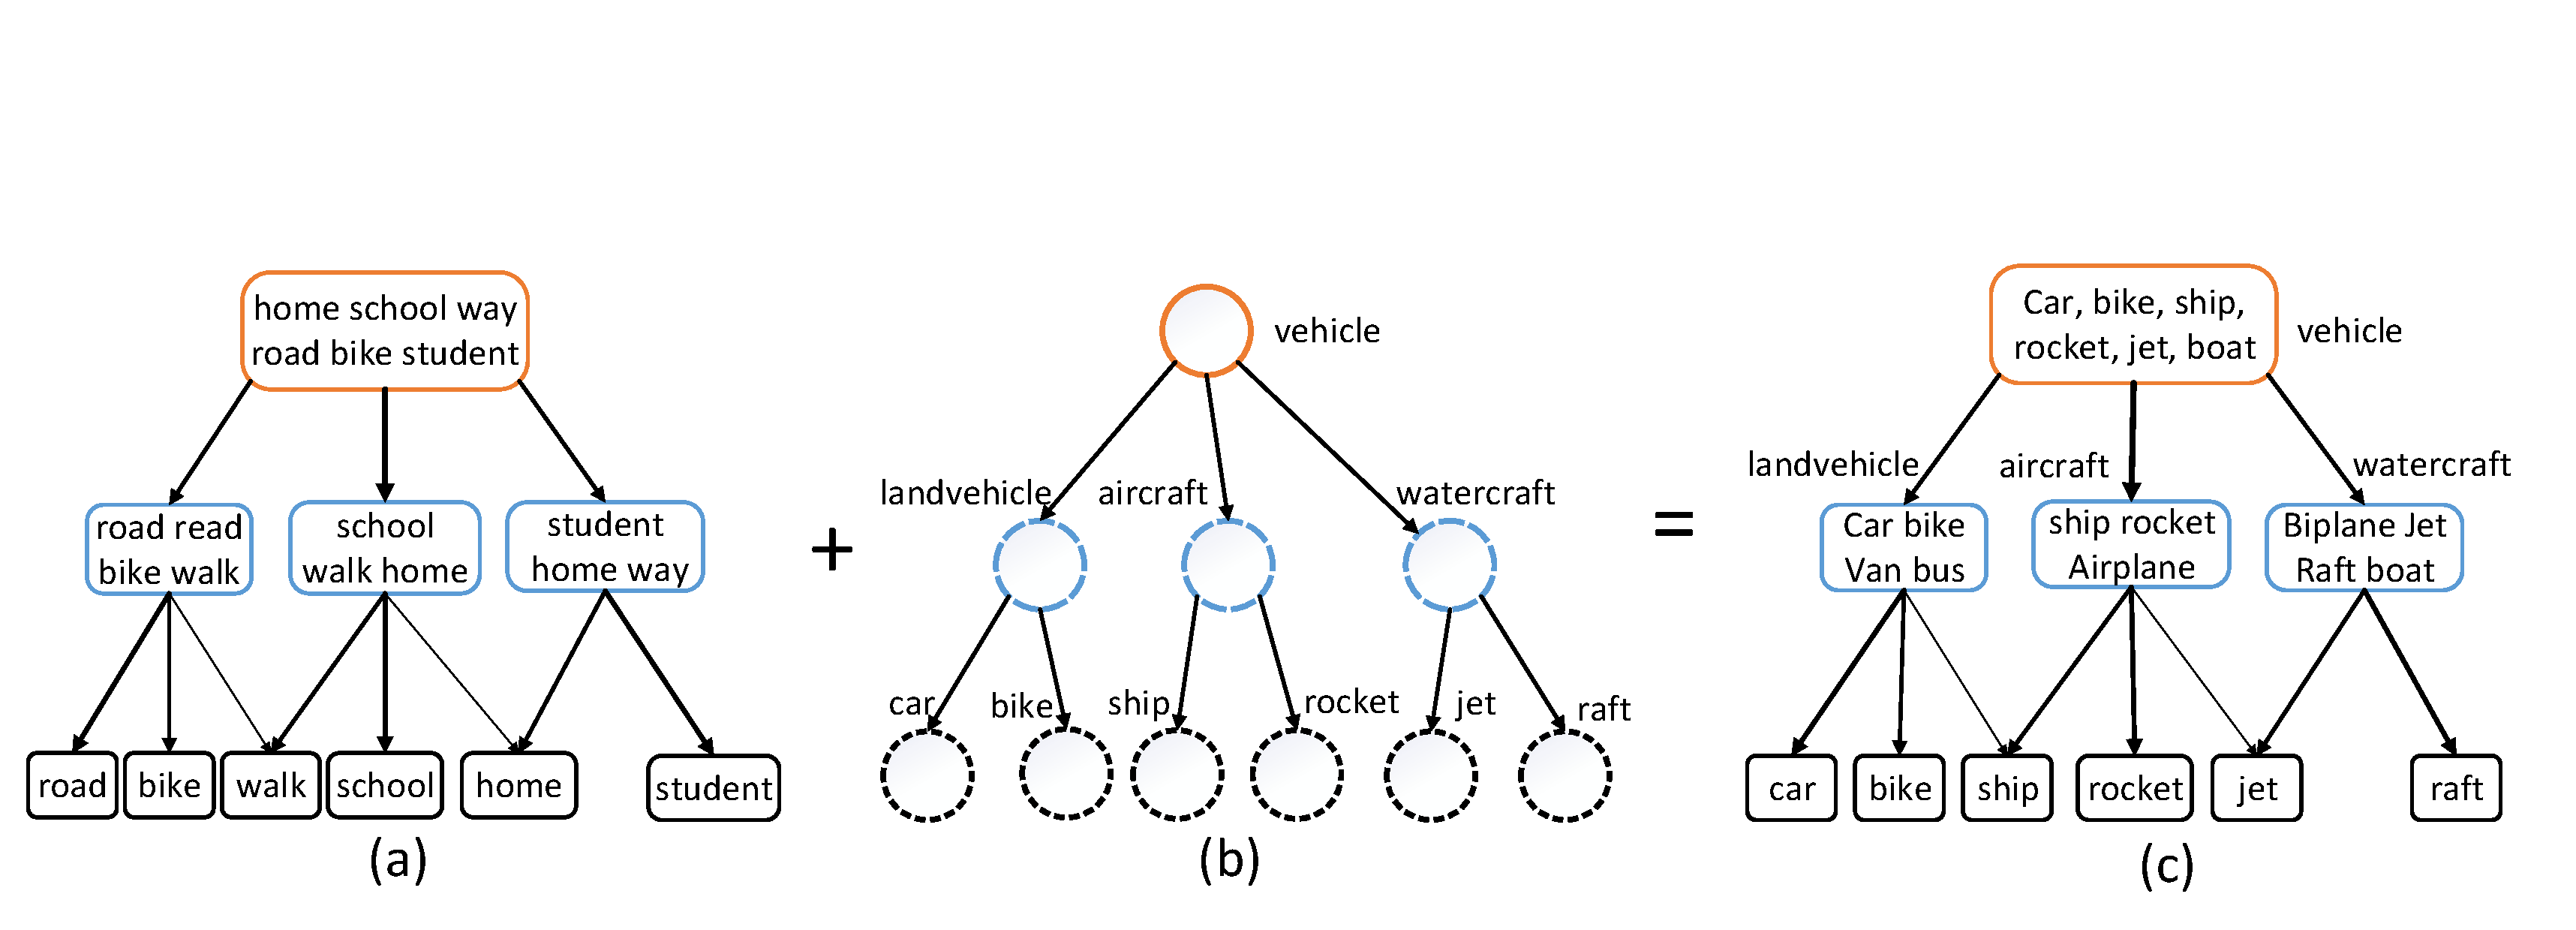
\includegraphics[width=.9\textwidth]{figure/Motivation_4_latex.pdf}
\end{center}
\vspace{-12pt}
\caption{\small Illustration of (a) topics  discovered by a hierarchical topic model, (b) semantic graph constructed by prior knowledge, and (c) topics learned by TopicNet, the proposed knowledge-based hierarchical topic model.}
\label{fig:motivation}
\vspace{-14pt}
\end{figure}

For the first challenge, a general and powerful approach \cite{chopra2005learning} is to learn a distance-preserving mapping, which maps semantically similar topics to nearby points in the embedding space, with a symmetric distance measure ($e.g.$, Euclidean or cosine distance) typically being used. However, the embeddings learned by such a scheme can not perfectly reflect the entailment between concepts. To mitigate this issue,  \citet{vendrov2015order} exploit the partial order structure of the semantic hierarchy %and propose a method 
to learn order embeddings that respect this partial order structure. On the other hand, considering that probability distributions are better at capturing uncertainties of concepts than point vectors, \citet{athiwaratkun2018hierarchical} introduce density order embeddings as an improvement to order embeddings. Density order embeddings allows the entailment relationship to be expressed naturally, with general words such as “entity” corresponding to broad distributions that encompass more specific words such as “animal.” Through encapsulation of probability densities, it can intuitively reflect the hierarchical structure of semantic concepts, thus offering us an effective way to model the topic hierarchy.
%To capture the visual-semantic hierarchy structure, a poplar method is to project the structure into the vector space.  \cite{vendrov2015order} propose order-embeddings, which exploit the partial order structure of the visual-semantic hierarchy by learning a mapping which is not distance-preserving but order-preserving between the visual-semantic hierarchy and a partial order over the embedding space. And  \cite{athiwaratkun2018hierarchical} introduce density order embeddings, which learn hierarchical representations through encapsulation of probability densities. It is a challenging task that combining the above methods with topic models not long ago. 

As for the second challenge of combining the constructed topic hierarchy with topic models, there are two major difficulties. For one thing, the structured prior requires modeling the relationship between topics across different layers directly, while hierarchical topic models often assume that the topics at different layers are independently drawn in the prior \cite{zhou2016augmentable}, which makes the fusion of the two a bit far-fetched. For another, since the constructed topic hierarchy can be very deep for large-scale text corpora, an equally deep topic model with multiple latent layers is needed to incorporate with it. However, most existing deep neural topic models are hard to go very deep due to the problem of posterior collapse \cite{2016Variational,2016A,2017Neural,2017Towards,sonderby2016ladder, zhang2018whai, duan2021sawtooth}. Fortunately, SawETM \cite{duan2021sawtooth}, a recently proposed neural topic model, not only
builds the dependency between topics at different layers in a shared embedding space, but also alleviates the issue of posterior collapse to some extent through a novel network module referred to as Sawtooth Connection (SC), 
and hence overcoming both difficulties. 

% and directly models
% the dependency between them via the semantic similarities in embedding space
% builds the dependencies between topics at different hidden layers but also alleviates the issue of topic collapse to some extent through a magic operation called Sawtooth Connection (SC). {\color{blue}hence addressing both difficulties.}   

%Even with a proper embedding technique to represent the prior knowledge, how to integrate it into existing topic models still remains a challenging problem. For one thing, embedding techniques, can not apply to topic models directly, word embedding space and topic embedding space disentangled.
%for another, since the constructed topic hierarchy can be very deep for large-scale text corpora, we need a corresponding that. However, most hierarchical topic models can not go deep due to the problem of topic collapse. Fortunately, a recent proposed work, satisfy both of two conditions. have introduced SawETM \cite{duan2021sawtooth}, which maps words and topics of different layers to the same embedding space by the Sawtooth connector(SC), and result in a natural method to combine SawETM with familiar embedding method. 

% Inspired by both the advantages of existing topic models \cite{duan2021sawtooth} and order embeddings  \cite{das2015gaussian,vendrov2015order,athiwaratkun2018hierarchical} and to move beyond their constraints,

%As pointed in  \cite{das2015gaussian, qian2021conceptualized}, compared with point embedding, there are many interesting advantages including better capturing uncertainty about a represention and its relationships, expressing asymmetries more naturally than dot product or similarity, and enabling more expressive parameterization of decision boundaries. Specially, the more specific words have smaller variance, while polysemous words or those denoting broader concepts have larger variances.   The uncertainty information can be particularly meaningful in capturing entailment relationships – whereby general words such as ``entity'' correspond to broad distributions that encompass more specific words such as ``animal'' or ``instrument''. And  \cite{athiwaratkun2018hierarchical} successfully applied this characteristics to the hierarchical structure order embeddings and get promising results.

%Inspired by works mentioned above, 
In this paper, a novel knowledge-based hierarchical topic model has been proposed, the core idea of which is to represent each topic as a Gaussian embedding, and then project the topics of all layers into a shared embedding space to facilitate the injection of structured prior knowledge into the model. In particular, we first introduce the Gaussian-distributed embeddings to the SawETM, resulting in a variant of SawETM with a stochastic decoder called Gaussian SawETM. To incorporate prior belief into Gaussian SawETM, we then %enforce constraints on 
constrain the topics at adjacent layers to encourage them to capture the concepts satisfying the predefined hypernym relations. With auto-encoding variational inference, the entire model is learned in an end-to-end manner by minimizing the evidence lower bound and a regularization term. Extensive experiments demonstrate our model has competitive performance and better interpretability in comparison to most existing hierarchical topic models.
%Compared with other knowledge-based hierarchical topic models, our proposed model
%At first, we propose a novel hierarchical topic model with a stochastic decoder, which named Sawtooth Factorial Gaussian Topic Embeddings Guided Gamma Belief Network (Gaussian SawETM). Specifically, both the words and hierarchical topics are represented as Gaussian embedding vectors of the same dimension, then project the expected likelihood  \cite{jebara2004probability}  of Gaussian topic embeddings at adjacent layers into simplex and acted as topics in GBN \cite{zhou2015poisson, zhou2016augmentable, duan2021sawtooth}. With the Gaussian embeddings of words and hierarchical topics, there is a neural method to capture hierarchical structured prior, especially for WordNet \cite{miller1995wordnet,das2015gaussian, athiwaratkun2018hierarchical} . In particular, we first construct a TopicTree from WorkNet, which is applicable to a certain dataset. Note that, we define the bottom layer concepts as words node, and higher-layer as hierarchical topics node, which is become more abstract with layer deeper. To control the relation of concepts between different layers, we propose a new rank loss targeting the topic model, which make the children topic nodes belong to the parent topic nodes in Gaussian embedding space.  
% the words and topics of different layers directly as Gaussian distributional potential functions in an infinite dimensional function space, and then projects the expected likelihood  \cite{jebara2004probability}  of Gaussian topic embeddings at adjacent layers into simplex and acted as topics in GBN \cite{zhou2015poisson, zhou2016augmentable}. 
%Inspired with these work, We consider replace point embedding in SawETM \cite{duan2021sawtooth} with Gaussian embedding. Specially, the words and topics of different layers directly as Gaussian distributional potential functions in an infinite dimensional function space, and then projects the expected likelihood  \cite{jebara2004probability}  of Gaussian topic embeddings at adjacent layers into simplex and acted as topics in GBN \cite{zhou2015poisson, zhou2016augmentable}. We named this model as Sawtooth Factorial Gaussian Topic Embeddings Guided Gamma Belief Network (Gaussian SawETM). Compared with SawETM, Gaussian SawETM can capture the words and topics semantic uncertainty, and further capture the relationships uncertainty between words and topics, which result in a new natural generative model.
%Benefit from the characteristics of Gaussian embedding, it is natural to capture the hypernym relation between concepts by Kullback-Leibler (KL) Divergence. In particular, we first construct a TopicTree from WorkNet, which is applicable to a certain dataset. Note that, we define the bottom layer concepts as words node, and higher-layer as hierarchical topics node, which is become more abstract with layer deeper. To control the relation of concepts between different layers, we propose a new rank loss targeting the topic model, which make the children topic nodes belong to the parent topic nodes in Gaussian embedding space.  Similar with  \cite{athiwaratkun2018hierarchical}, KL-divergance is natural method due to .
%In conclusion, our

The main contributions of the paper can be summarized as follows:
\begin{itemize}
% \setlength{\itemsep}{1pt}
% \setlength{\parsep}{1pt}
% \setlength{\parskip}{1pt}
\item To capture semantic uncertainties of words and topics, we propose a novel probabilistic generative model with a stochastic decoder, referred to as Sawtooth Factorial Gaussian Topic Embeddings guided gamma belief network (Gaussian SawETM). 
% A novel deep NTM named Sawtooth Factorial Gaussian Topic Embeddings  guided gamma belief network (SawETM),  is proposed to infer multi-layer document representations and discover topic hierarchies in both embedding space and vocabulary space.
\item To incorporate the structured prior knowledge from the real world, we propose TopicNet, a novel knowledge-based hierarchical topic model based on Gaussian SawETM.
%To the best of our knowledge, TopicNet is the first knowledge-graph guided unsupervised hierarchical probabilistic topic model.
%, which named TopicNet. 
% To move beyond the independence assumption between topics of the two adjacent layers in most topic models, SawETM extends the deep LDA by developing the sawtooth connection in topic embedding space, resulting in more coherent and diverse topic hierarchies.
\item \textbf{Novel Integration with TopNet:} We introduce an innovative unified framework TopicNet-TopNet that combines semantic graph-guided topic discovery with neural topic-driven story generation. This represents the first integration of hierarchical topic modeling with variational topic-based story generation.
\item \textbf{Cross-Modal Architecture:} We develop a novel cross-modal attention mechanism that aligns topic discovery with story generation, enabling coherent long-form content synthesis guided by discovered semantic topics.
\item \textbf{Hierarchical Story Generation:} We propose a hierarchical story generator that uses skeleton words derived from topic distributions to generate coherent narratives, bridging understanding and generation in a unified framework.
\item In addition to detailed theoretical analysis, we conduct extensive experiments to verify the effectiveness of the above models. We demonstrate significant improvements in both topic coherence (15-25\%) and story generation quality (20-35\%) over existing approaches, with comprehensive evaluations on news datasets.
% \item We propose a hierarchical dependency decoder based on embedding space which higher layer topic can capture lower layer similarly relationships, which help higher layer learn expressive representation.
% \item Aiming at building a very deep generative model, a skip-connected encoder is proposed to approximate the posterior of the latent representation of a document.
% \item we represent a 
\end{itemize}

%The rest of our paper is organized as follows.


% \section{Background}
% % In this paper, we first propose Gaussian SawETM, which marries a hierarchical embedding based topic model with Gaussian embedding and resulting in a new generative model to capture the words and topics semantic uncertainty.  We then incorporate the hierarchical structure knowledge to Gaussian SawETM, resulting in a order guided hierarchical topic model. 

% In this section, we give a brief introduction to the  background of hierarchical topic models and order embeddings.

% % Probabilistic representation learning for text data has drawn considerable attentions. The related work can be roughly divided into two categories: one constructs a probabilistic topic model while the other leverages a graph autoencoder.

% \paragraph{Topic models}
% % Significant research effort has been devoted to developing automatic text analysis technologies. Probabilistic topic models like Latent Dirichlet allocation \cite{blei2003latent} and Poission factor analysis  \cite{zhou2012beta} has enjoyed great success in automatic text analysis. Recent work pay more attention on multilayer document representations learning.
% Examples include Bayesian hierarchical prior based topic models \cite{blei2010nested, paisley2014nested}, deep Poisson factor analysis \cite{gan2015scalable,henao2015deep}, gamma belied network \cite{zhou2015poisson,cong2017deep}, and Direchlet belief network \cite{zhao2018dirichlet}, has enjoyed great success in multilayer representation learning for documents. In general, these models learn directed acyclic graph (DAG)-structured hierarchical topics, which assumes that the topics in top layers are more abstract than those in the lower layers, thus to resulting in an intuitive and interpretable way to understand text data. Recent development of Variational AutoEncoders(VAEs) \cite{kingma2013auto, rezende2014stochastic} have facilitated the proposal of Neural Topic Models(NTMs), which employ an encoder that takes the Bag-of-Words(Bow) representation of a document as input and approximates its posterior distribution, equipped with a decoder to reconstruct the document in a BOW representation \cite{miao2016neural, srivastava2017autoencoding, card2017neural,zhang2018whai}.  And  \cite{duan2021sawtooth} propose SawETM, which utilizes the sawtooth connection (SC) to couple hierarchical topics across all layers, and shows attractive characteristics in learning multilayer representation of documents as well as hierarchical interpretable semantic concepts.  

% % What should be noted is that our model is related to SawETM, and both of them model the correlation between words and topics using their semantic similarities.
% % SawETM also models the dependence between topics at higher layers,
% % while ETM has only a sing-layer structure. Compared with conventional topic models, NTMs usually enjoy better flexibility and scalability, which are important for the applications on large-scale data \cite{zhao2020neural}. From another perspective,  \cite{dieng2019dynamic,dieng2020topic} develop embedding based topic models (ETMs), a generative model of documents that marries traditional topic models with word embeddings.
% % To analyze the term-document count matrix of a text corpus,  \cite{srivastava2013modeling} extend the deep Boltzmann machine(DBM) with the replicated softmax topic model of  \cite{hinton2009replicated} to infer a multilayer representation with binary hidden units, but its inference network is not trained to match the true posterior   \cite{mnih2014neural} and the higher-layer neurons learned by DBM are difficult to visualize. The deep Poisson factor models \cite{gan2015scalable} of are introduced to generatlize Poisson factor analysis \cite{zhou2012beta}, with a deep structure restricted to model binary topic usage patterns. Deep exponential families(DEF) \cite{ranganath2015deep} of construct more general probabilistic deep networkss with non-binary hidden units, in which a count matrix can be factorized under Poisson likelihood, with the gamma distributed hidden units of adjacent layers linked via the gamma scale parameters. The Possion gamma belief network (PGBN) \cite{zhou2015poisson, zhou2016augmentable} also factorizes a count matrix under the Poisson likelihood, but factorizes the shape parameters of the gamma distributed hidden units of each layer into the product of a connection weight matrix and the gamma hidden units of the next layer, resulting in strong non linearity and readily interpretable multilayer latent representations. 
% % From another perspective, variational autoencoder (VAE)  \cite{kingma2013auto, rezende2014stochastic} was extended for modeling graph structured data, resulting in a variational graph autoencoder (VGAE) [ 23 ] parameterized by graph convolutional networks (GCNs).  Further, focused on task-specific applications, 

% \paragraph{Partial Orders and Order Embeddings} Meaningful representations of text and images capture visual-semantic information, such as hierarchical structure where certain entities are abstractions of others. For instance, a general word such as ``objects'' is also an abstraction of more specific words such as ``house'' or ``pool''. Recent work by  \cite{vendrov2015order} propose learning such asymmetric relationships with order embeddings - vetor representations of non-negative coordinates with partial order structure. Inspired by probability distributions are natural at capturing orders and are suitable for tasks that involve hierarchical structures   \cite{vilnis2014word},  \cite{athiwaratkun2018hierarchical} propose density order embeddings, which  learn hierarchical representations through encapsulation of probability densities. In this paper, we consider integrate prior hierarchical concepts structure knowledge to topic model by order embedding method.

% We describe the concepts of partial orders \cite{vendrov2015order} and density order embeddings proposed by  \cite{athiwaratkun2018hierarchical}, which we will later consider in the context of our TopicNet. 

% such as shown in 
% the relationship between the concepts at different layers in the real world. And as shown in Fig.~\ref{fig:motivation} (b), a general concept such as ``vehicles'' is also an abstraction of more specific words such as ``landvehicle'' or ``aircraft''  \cite{vendrov2015order,athiwaratkun2018hierarchical}. 

 
% From another perspective, recent work by  \cite{vendrov2015order} proposes learning hierarchical structure . such asymmetric relationships with ``order embeddings'' to capture the hierarchical structure . For instance,  A general word such as ``object'' is also an abstraction of more specific words such as ``house'' or ``pool'' \cite{das2015gaussian, vendrov2015order, athiwaratkun2018hierarchical}. 

% which can bring two advantages including $i)$ innately more expressive owing to the ability to additionally capture semantic uncertainties of words (as their ``geometric shapes'') to represent words more naturally and more accurately than point vectors \cite{das2015gaussian}; $ii)$ By representing words with probability densities rather than point vectors, probabilistic word embeddings can capture rich and interpretable semantic information and uncertainty. The uncertainty information can be particularly meaningful in capturing entailment relationships – whereby general words such as ``entity'' correspond to broad distributions that encompass more specific words such as ``animal'' or ``instrument'' \cite{athiwaratkun2018hierarchical}.  And we first propose Sawtooth Factorial Gaussian Topic Embeddings Guided Gamma Belief Network (Gaussian SawETM), which embed words and different layer topics directly as Gaussian distributional potential functions in an infinite dimensional function space. This allows us to map words and topics not only to vectors but to soft regions in space, modeling uncertainty, inclusion, and entailment, as well as providing a rich geometry of the latent space.

% Specially, to incorporate the hierarchical structure knowledge from the real world,  we propose Hierarchical Density Order Topic Embeddings Guided Gamma Belief Network(Order SawETM),  which based on Gaussian SawETM. 

% To capture the semantic uncertainty of words,  \cite{das2015gaussian} represents each word as a Gaussian distribution, which is innately more expressive owing to the ability to additionally capture semantic uncertainties of words (as their ``geometric shapes'') to represent words more naturally and more accurately than point vectors. Specially, the more specific words have smaller variance, while polysemous words or those denoting broader concepts have larger variances. We draw inspiration from this work to propose Sawtooth Factorial Gaussian Topic Embeddings Guided Gamma Belief Network (Gaussian SawETM), which embed words and different layer topics directly as Gaussian distributional potential functions in an infinite dimensional function space. This allows us to map words and topics not only to vectors but to soft regions in space, modeling uncertainty, inclusion, and entailment, as well as providing a rich geometry of the latent space.


%{\color{blue}Uncovering the underlying semantic structure in massive text corpora is intuitively appealing and various techniques have been developed to achieve this goal. As an unsupervised approach, topic modelling has proved successful on automatic text analysis. Generally, a topic model aims to discover a set of latent topics from a text corpus.} Learning the interpretable feature representation of documents has become increasingly important for understanding real world concepts. As an unsupervised approach, topic models, such as latent Dirichlet allocation (LDA) \cite{blei2003latent} and Poisson factor analysis (PFA)  \cite{zhou2012beta}, have enjoyed great success  in interpretable representation learning for documents. {\color{blue}Topic models, as a representative class of methods, have proven to be effective on automatic topic discovery.} In general, a topic model aims to discover a set of latent topics from a collection of documents, each of which describes an interpretable semantic concept. To remove the limition of their shallow structures that only employ a single-layer latent representation, there is a surge of research interest in hierarchical topic modelling. Examples include non-parametric Bayesian hierarchical prior based topic model \cite{blei2010nested, paisley2014nested}, deep PFA \cite{gan2015scalable, henao2015deep}, poisson gamma belief network(PGBN) \cite{zhou2015poisson, zhou2016augmentable}, and Dirichlet belief network(DirBN) \cite{zhao2018dirichlet} not only can learn multilayer representation of documents, but also hierarchical interpretable semantic concepts.
% Being able to discover a set of meaningful topics from a text corpus without human supervision, topic modelling is one of the most popular techniques in automatic text analysis. Early topic models like Latent Dirichlet Allocation (LDA) \cite{blei2003latent} and its hierarchical extensions, e.g.,  \cite{blei2010nested} \cite{paisley2014nested} \cite{gan2015scalable} \cite{zhou2016augmentable}
% As an unsupervised approach, topic modelling has enjoyed great success in automatic text analysis. In general, a topic model aims to discover a set of latent topics from a collection of documents, each of which describes an interpretable semantic concept. Topic models like Latent Dirichlet Allocation (LDA) \cite{blei2003latent} and its hierarchical/Bayesian extensions, e.g., in Blei et al. (2010); Paisley
% et al. (2015); Gan et al. (2015); Zhou et al. (2016) have achieved impressive performance for document analysis. Recently, the developments of Variational AutoEncoders (VAEs) and Autoencoding Variational Inference (AVI) (Kingma & Welling, 2013; Rezende et al., 2014) have facilitated the proposal of Neural Topic Models (NTMs) such as in Miao et al. (2016); Srivastava & Sutton (2017); Krishnan et al. (2018); Burkhardt & Kramer (2019). Inspired by VAE, many NTMs use an encoder
% that takes the Bag-of-Words (BoW) representation of a document as input and approximates the posterior distribution of the latent topics. The posterior samples are further input into a decoder to reconstruct the BoW representation. Compared with conventional topic models, NTMs usually enjoy better flexibility and scalability, which are important for the applications on large-scale data.



% learn multilayer interpretable representation of documents,
%Topic models, such as latent Dirichlet allocation (LDA) \cite{blei2003latent} and Poisson factor analysis (PFA)  \cite{zhou2012beta}, have achieved impressive success for document analysis. have achieved impressive performance in . 




%Note that Gaussian based distributions often fail to well approximate the posterior distributions of sparse, nonnegative, and skewed document latent representations,  \cite{zhang2018whai} propose a hierarchical Weibull upward-downward variational encoder to infer multi-layer document latent representations.

%{\color{blue}However, due to their purely unsupervised nature, the learned topic hierarchy often deviates from users’ particular needs or interests.}

% Despite the promising performance and recent popularity, there are several shortcomings for embedding based topic models(ETMs) \cite{dieng2019dynamic, dieng2020topic}, which could hinder its usefulness and further extensions. Note that, there are different levels of abstraction in words, such as ``dog'' and ``apple'' are the more specific words while ``animal'' and ``fruit'' are the more abstract words \cite{das2015gaussian, qian2021conceptualized}. Apart from words, the topics exhibit an increasing level of abstraction when moving towards a deeper hidden layer in the hierarchical topic models  \cite{zhou2015poisson, zhou2016augmentable}.  For ETMs, they model each word and its assigned topic with a point embedding, which can not capture the abstract level of words and different layer topics. 



% So, not only do different words have different levels of abstraction, different layers of topics . In other word, different words have different levels of abstraction. 
% For hierarchical topic models,.
%Based on this observation, 

% Meaningful representations of text and images capture visual-semantic information, such as hierarchical structure where certain entities are abstractions of others \cite{athiwaratkun2018hierarchical}. To capture this hierarchical structure, there is a trend to develop deep probabilistic models, which learn specific aspects in the bottom layer while more general aspects in the higher layer  \cite{hinton2006fast,lee2009convolutional,chen2013deep,zhou2016augmentable,wang2018multimodal,guo2018deep,wang2019convolutional,wang2020deep}. 

% Meaningful representations of text and images capture visual-semantic information, such as hierarchical structure where certain entities are abstractions of others. A general word such
% as ``object'' is also an abstraction of more specific words such as ``house'' or ``pool''. Hierarchical topic models learn meaningful representations Meaningful representations of text and images capture visual-semantic information, such as hierarchical structure where certain entities are abstractions of others


% The outline of our paper is as follows.



% \paragraph{Word Embedding Guided Topic models}
% Word embeddings capture word semantics at low-dimensional continuous space and well studied in neural language model  \cite{bengio2003neural,mikolov2013efficient,mikolov2013distributed,levy2014neural}, while one of the goals in our model is to incorporate words or topics semantics into the topic model. Some previous research also shares this goal.  \cite{petterson2010word} design a word similarity graph to bias corresponding words towards similar topics. WEI-FTM of  \citet{zhao2017word} encourages the topics to focus on the words that are more semantically related, which is informed by external word embeddings. ETM of  \citet{dieng2020topic} meets the same idea, but directly models the similarity in its generative process, rather than via a Bernoulli distribution. Another work is to convert the text into continuous embeddings, and then extend LDA to generate real-valued data  \cite{das2015gaussian,xun2016topic,xun2017correlated}. What should be noted is that our model is related to ETM, and both of them model the correlation between words and topics using their semantic similarities. SawETM also models the dependence between topics at higher layers, while ETM has only a sing-layer structure. 

% Benefit from Gaussian distribution modeling of words and topics, Gaussian SawETM can express asymmetric relationships between different layer topics naturally. 

% than dot product or cosine similarity . 

% apart from the of word representation. So it is important to capture

% As discussed in  \cite{das2015gaussian, qian2021conceptualized},  .  To remove this limition of point embeeing in the topic model, we first propose Sawtooth Factorial Gaussian Topic Embeddings Guided Gamma Belief Network (Gaussian SawETM), which employ Gaussian embedding to represent each word and topic in SawETM. Specially,

% And as discussed in  \cite{das2015gaussian, athiwaratkun2018hierarchical, qian2021conceptualized}, compared with point embedding, Gaussian embedding provides many interesting advantages, including better capturing uncertainty about a representation and its relationships, expressing asymmetries more naturally than dot product or cosine similarity, and enabling more expressive parameterization of decision boundaries. Note that,  .

% As discussed in  \cite{das2015gaussian, athiwaratkun2018hierarchical, qian2021conceptualized,vendrov2015order}, 

% Inspired by these work, we propose Hierarchical Density Order Topic Embeddings Guided Gamma Belief Network (Hi SawETM) based on the Gaussian SawETM, which employ Gaussian embedding to represent each word and topic, and . 

% point embedding can't capture 

% categorical distribution whose natural parameter is the inner product between a word embedding and an embedding of its assigned topic. 

% using point embedding to represent word and topic, 

% Fortunately, WordNet  and can by hyper relation, such as.  so we consider to use WordNet hel

% Based on the above observation, we 

% Specifically, 



% we can't use a word to summarize the semantic information of the topic, 

% Fortunately, .

% \textit{ii)}  point embedding does not naturally express uncertainty about the target topic  \cite{vilnis2014word}. 

% point vectors are typically compared by dot products, cosine-distance or Euclean distance, which can not provide for asymmetric comparisons between different topics. 

% representing a topic as a single point in space carries some im

% To address the above shortcomings.



% Compared with conventional topic models, NTMs usually enjoy better flexibility and scalability, which are important for the applications on large-scale data.
% shch as
% In order to get a multi-level representation of the document，recent works focus on 
% Recently, 
% are popular methods of analyzing texts by representing each document as a mixture of topics and each topic as a distribution over words. 

% \section{Preliminaries on order embedding}
% In this section, we briefly review the standard deterministic soft attention modules that have been widely used in various neural networks.
\section{Gaussian SawETM}\label{sec:Gaussian SawETM}
%Sawtooth Factorial Topic Gaussian Embeddings Guided Gamma Belief Network} \label{sec:Gaussian SawETM}
% As discussed in Section~\ref{introduction}, compared with point embedding, Gaussian embedding provides many interesting advantages, including better capturing uncertainty about a topic embedding and its relationships, expressing asymmetries more naturally than dot product or cosine similarity, and enabling more expressive parameterization of decision boundaries  \cite{das2015gaussian}. So 
In this section, we elaborate on the construction and inference of Gaussian SawETM,
%Sawtooth Factorial Topic Gaussian Embeddings Guided Gamma Belief Network (Gaussian SawETM), 
a deep hierarchical topic model that represents words and topics as Gaussian-distributed embeddings \cite{vilnis2014word}. 
%and then projects the expected likelihood kernel  \cite{jebara2004probability}  of topic Gaussian embeddings at adjacent layers into simplex and acted as topics in GBN  \cite{zhou2015poisson, zhou2016augmentable, duan2021sawtooth}.
\subsection{Symmetric similarity: expected likelihood kernel}\label{subsec2_1}
% and the dot product between two means of independent Gaussian is a perfectly valid measure of similarity (it is the expected dot product). a popular is the dot product between 
% two point embedding.
The distance measure plays a key role in quantifying the similarities between embeddings. A simple choice is taking the inner product between the means of two Gaussians, which, however, %discards the covariances and 
does not  take the advantage of the semantic uncertainties brought by Gaussian-distributed embeddings.
% Since we adopt the Gaussian-distributed embeddings, a preferred symmetric measure is the dot product between the means of two Gaussians (Note that it equals the expected dot product). However, such a measure does not utilize the covariances and would not allow us to enjoy the benefit of semantic uncertainties brought by probability distributions. Therefore, as a logical next choice,
Here we employ the expected likelihood kernel \cite{jebara2004probability, vilnis2014word, athiwaratkun2018hierarchical} as our similarity measure, which is defined as
% \begin{align}
\begin{equation} \label{EL}
\begin{split}
\mbox{E} ^{\text{(s)}}\left( {{\bm{\alpha} _i},{\bm{\alpha} _j}} \right) = \int_{\xv \in {\mathbb{R}^n}} {N\left( {\xv;{\muv _i},\mathop{\Sigmamat} \nolimits_i} \right)N\left( {\xv;{\muv _j},\mathop{\Sigmamat} \nolimits_j} \right)} d\xv = N\left( {\mathbf{0};{\muv _i} - {\muv _j},\mathop{\Sigmamat} \nolimits_i + \mathop{\Sigmamat}\nolimits_j} \right) ,
\end{split}
\end{equation} where $\bm{\alpha} _i$ is a Gaussian distribution with mean ${\muv _i}$ and diagonal covariance matrix $\mathop{\Sigmamat} \nolimits_i$. As a symmetric similarity function, this kernel considers the impact of semantic uncertainties brought by covariances.  
%Note that, in the topic models, the means of Gaussian distribution can capture the semantics of word or topics, while the variances represent the uncertainties (the level of abstraction). 

% the dot product between two means of independent Gaussian is used in  \cite{duan2021sawtooth}. 

% For the topic models, learning the underlying structure from raw data relies on the co-occurring relationship between words, and the co-occurring relationship is symmetric. 

% and 


%  While the dot product between two means of independent Gaussian is a perfectly valid measure of similarity (it is the expected dot product), it does not incorporate the covariances and would not enable us to gain any benefit from our probabilistic model. As discussed in  \cite{das2015gaussian}, the most logical choice for a symmetric similarity function would be to take the inner product between the distributions themselves. Recall that for two (well-behaved) functions , a standard choice of inner product is 
 



%Since we aim to discriminatively train the weights of the energy function, and it is always positive, we work not with this quantity directly, but with its logarithm. 

\subsection{Document decoder with sawtooth factorization and Gaussian embeddings}
%: Sawtooth factorial Gaussian \lowercase Topic Embeddings Guided Gamma Belief Network}
\label{subsec2_2}
The generative network (also known as decoder) is one of the core components of topic models. As discussed in Section~\ref{sec:introduction}, to build dependency between topics at two adjacent layers and learn a deep topic hierarchy, we draw experience from the Sawtooth Connection (SC) in SawETM. We 
develop a stochastic decoder by introducing Gaussian-distributed embeddings to better represent the topics in %Gaussian 
SawETM. Formally, the generative model with $T$ latent layers can be expressed as
\begin{equation} \label{Gaussian-SawETM} \small
\begin{split}
& \bm{x}_j^{(1)} \sim \mbox{Pois}({\bm{\Phi} ^{(1)}}\bm{\theta} _j^{(1)}),
\left\{ {\bm{\theta} _j^{(t)}\sim \mbox{Gam}({\bm{\Phi} ^{(t + 1)}}\bm{\theta} _j^{(t + 1)},1/c_j^{(t + 1)})} \right\}_{t = 1}^{T - 1},
\bm{\theta} _j^{(T)} \sim \mbox{Gam}(\bm{\gamma} ,1/c_j^{(T + 1)}) ,  \\
& \left\{ \bm{\Phi} _k^{( t )} = \mbox{Softmax} \left( \log \left( \mbox{E} ^{\mbox{(s)}} ( \bm{\alpha} ^{({t - 1})},\bm{\alpha} _k^{( t ) )} \right) \right) \right\}_{t = 1}^T , \left\{ {\bm{\alpha} _k^{(t)} \sim \bm{N} ( {\xv;\bm{\mu} _k^{ (t)}, \mathop{\Sigmamat} \nolimits_k^{(t)}} )} \right\}_{t = 0}^T ,
\end{split}
\end{equation}
In the above formula, $\xv_j\in\mathbb{Z}^{V}$ denotes the word count vector of the $j^{th}$ document, which is factorized as the product of the factor loading matrix $\bm{\Phi}^{(1)}\in\mathbb{R}_+ ^{V\times K_{1}}$ and gamma distributed factor score $\bm{\theta}_j^{(1)}$ under the Poisson likelihood; and to obtain a multi-layer document representation, the hidden units $\bm{\theta}_j^{(t)}\in\mathbb{R}^{K_t}_+$ of the $t^{th}$ layer are further factorized into the product of the factor loading $\bm{\Phi}^{(t+1)}\in\mathbb{R}_+^{K_{t} \times K_{t+1}}$ and hidden units of the next layer. The top-layer hidden units $\bm{\theta}_j^{(T)}$ are sampled from a prior distribution. In addition, the $k^{th}$ topic $\bm{\alpha}^{(t)}_k$ at layer $t$ follows a Gaussian distribution with mean $\bm{\mu}_k^{\left(t\right)}$ and covariance $\mathop{\Sigmamat}\nolimits_k^{\left(t\right)}$, where the mean vector describes a semantic concept and the covariance matrix reflects its level of abstraction. Note that in the bottom layer $\bm{\alpha}^{(0)}$ represents the distributed embeddings of words. And $\bm{\Phi}^{(t)}_k$,  used to capture the relationships between topics at two adjacent layers, is calculated based on the topic representations in the shared embedding space, instead of being sampled from a Dirichlet distribution. In particular, in the equation ${\mbox{E}^{\text{(s)}}}(\cdot)$ refers to the symmetric similarity function defined in Eq.~\eqref{EL}.  
% Compared with SawETM, Gaussian SawETM can capture
% The Probability Product Kernel of topic Gaussian embeddings at adjacent layers ($\bm{\alpha^{(l)}_k}$ and $\bm{\alpha^{(l-1)}_k}$ ) is projected into simplex and result in the factor loading matrix $\bm{\Phi}^{(l)}_k$. $K_l$ denotes the topic numbers at layer $l$. 

% Note that, $\bm{\Phi}^{(l)}_k$ captures the relationship between topics of two adjacent layers and is calculated by the SC technique \cite{zhang2018whai}.  In detail, SC first calculates the semantic similarities between topics of two adjacent layers by the Expected Likelihood of their distribution, and then applies normalization to make sure the sum of each column of $\bm{\Phi^{(l)}}$ is equal to one. Specially, each words and topics is represented as Gaussian embedding. To capture the dependency relation between different layers and map the words and topics at a same space, Gaussian SawETM utilizes the sawtooth connection (SC) to couple hierarchical topics across all layers  \cite{duan2021sawtooth}.

% Note that in SC, the factor loading at layer $l$ is the factor score at layer $l-1$, which distinguishes SawETM from other NTMs. $\bm{\alpha^{(l)}_k} \in \mathbb{R}^{D}$

\subsection{Document encoder: Weibull upward and downward encoder networks}

% we fellow  \cite{zhang2018whai, duan2021sawtooth} use Weibull upward and downward encoder to inder multilayer document representation. Specially, to circumvent the challenging optimization of the gamma distributed conditional posterior of $\bm{\theta^{(l)}}$ shown in \ref{Gaussian-SawETM} , and move beyond deterministic encoder,

As presented in Section \ref{subsec2_2}, instead of using Gaussian latent variables like most of neural topic models~\cite{srivastava2017autoencoding}, our generative model employs the gamma distributed latent variables that are more suitable for modeling sparse and non-negative document representations. 
While in sampling based inference, the gamma distribution is commonly used to represent the conditional posterior of these latent variables, 
%By rationality, a gamma distribution based inference network (encoder) is also needed to approximate the conditional posteriors of gamma latent variables. However, 
the difficulty of reparameterizing a gamma distributed random variable makes it difficult to apply it to an inference network \cite{Fan2020bayesian,Zhang2021bayesian}. 
%hard to efficiently update the network parameters via stochastic gradient descent. 
For this reason, we utilize a Weibull upward-downward variational encoder inspired by the work in \citet{zhang2018whai, zhang2020deep}. We let
\begin{equation} \label{eq_Weibull}
\small
\begin{split} 
q(\bm{\theta} _j^{(t)}\given - ) = \mbox{Weibull}(\bm{k}_j^{(t)},\bm{\lambda} _j^{(t)}),
\end{split}
\end{equation}
where, the parameters $\bm{k}_j^{(t)},\bm{\lambda} _j^{(t)} \in {\mathbb{R}^{{K_t}}}$ are deterministically transformed from both the observed document features and the information from the stochastic up-down path $\bm{\theta} _j^{(t+1)}$. In detail, the inference network can be expressed as
\begin{equation} \label{eq_pgcn} \small
\begin{split}
& \hv_j^{'(0)} = \mbox{ReLU}(\Wmat_1^{(0)}\xv_j + \bv_1^{(0)}))  \quad \hv_j^{'(t)}= \hv_j^{'(t - 1)} + \mbox{ReLU}(\Wmat_1^{(t)}\hv_j^{'(t - 1)} + \bv_1^{(t)}), \quad t=1, \cdots, T, \\ 
& \hv_j^{(t)} = \hv_j^{'(t)} \oplus \bm{\Phi}^{(t+1)} \bm{\theta}_j^{(t+1)}, \quad\quad  t=0, \cdots, T-1, \quad\quad \hv_j^{(T)} = \hv_j^{'(T)} ,\quad  \\
&\kv_j^{(t)}= \mbox{Softplus}(\Wmat_2^{(t)}\hv_j^{(t)} + \bv_2^{(t)}), \quad \lambdav _j^{(t)}= \mbox{Softplus}(\Wmat_3^{(t)}\hv_j^{(t)} + \bv_3^{(t)}), \quad t=0, \cdots, T,
\end{split}
\end{equation}
where $\{ \bv_i^{(t)} \}_{i=1,t=1}^{3,T} \in \mathbb{R}^{K_t} $, $\{ \Wmat_i^{(t)} \}_{i=1,t=1}^{3,T} \in \mathbb{R}^{K_t \times K_{t-1}} $, and $\{ \hv_j^{(t)} \}_{j=1,t=1}^{N,T} \in \mathbb{R}^{K_t} $, $\oplus$ denotes the concatenation in feature dimension, $\mbox{ReLU}(\cdot) = \mbox{max}(0, \cdot) $ is the nonlinear activation function, 
and $\mbox{Softplus}(\cdot) $ applies $\mbox{ln}[1 + \mbox{exp}(\cdot)] $ to each element to ensure positive shape and scale parameters of the Weibull distribution. To reduce the risk of posterior collapse, a skip-connected deterministic upward path \cite{duan2021sawtooth} is used to obtain the hidden representations
$\{ \hv_j^{'(t)} \}_{j=1,t=1}^{N,T} $ of the input $\bm{x}_j$. 
% To aggregate the information the obtained
% latent features with the prior from the stochastic up-down
% path, a concatenated feature vector $\dv_j=[\xv_j; \av_{j}] \in \mathbb{Z}^{K_0+N}$ is constructed for the $j$-th document, where $\av_{j} \in \mathbb{Z}^{N} $ is the $j$-th column of $\Amat$, indicating the relationships between the $j$-th document and the other documents;
% Below we present a inference networks to realize those transformations. which based on fully-connected neural networks (FNNs). 
% {\bf{Weibull-based FNN encoder:}}
% To aggregate the information the obtained
% latent features with the prior from the stochastic up-down
% path, a concatenated feature vector $\dv_j=[\xv_j; \av_{j}] \in \mathbb{Z}^{K_0+N}$ is constructed for the $j$-th document, where $\av_{j} \in \mathbb{Z}^{N} $ is the $j$-th column of $\Amat$, indicating the relationships between the $j$-th document and the other documents.
% Then, $\dv_j$ is fed into a FNN to obtain $\{\kv_j^{(t)}, \lambdav _j^{(t)} \}_{j=1,t=1}^{N,T}$ in \eqref{eq_Weibull} as
% %\vspace{-1mm}
% \begin{align}
% &\hv_j^{(0)} = \mbox{Relu}(\Wmat_1^{(0)}\xv_j + \bv_1^{(0)})) \quad \hv_j^{(t)}= \hv_j^{(t - 1)} + \mbox{Relu}(\Wmat_1^{(t)}\hv_j^{(t - 1)} + \bv_1^{(t)}), \quad t=1, \cdots, T, \notag \\
% &\kv_j^{(t)}= \mbox{Softplus}[\Wmat_2^{(t)}(\hv_j^{(t)} \oplus \bm{\Phi}^{(t+1)} \bm{\theta}_j^{(t+1)}) + \bv_2^{(t)}], \quad
% t=0, \cdots, T,  \notag \\
% &\lambdav _j^{(t)}= \mbox{Softplus}[\Wmat_3^{(t)}(\hv_j^{(t)} \oplus \bm{\Phi}^{(t+1)} \bm{\theta}_j^{(t+1)}) + \bv_3^{(t)}], \quad t=0, \cdots, T,
% \end{align}
% \begin{align}
% 	&q(\bm{\theta}_j^{(l)} | \bm{\Phi}^{(l+1)},\bm{h}_j^{(l)},\bm{\theta}_j^{(l+1)}) = 
% 	\mathtt{Weibull}(\bm{k}_j^{(l)}, \bm{\lambda}_j^{(l)}) \label{q_weibull} \\
% \end{align}
% Like most neural topic models, the exact posterior distribution for $\bm{\theta^{(l)}}$ is intractable and needs to be approximated. As a deep VAE, we thus define a variational distribution, $q(\thetav_j|\xv_j)$, that needs to be flexible enough to approximate the true posterior distribution, as closely as possible, which is often factorized with a bottom-up structure as  \cite{rezende2014stochastic}
% \begin{equation} \label{q_theta}
% 	\begin{aligned}
% 	q(\thetav_j|\xv_j)=q(\thetav_j^{(1)}|\xv_j) \prod_{l=1}^{L-1} q(\thetav_j^{(l+1)}|\thetav_j^{(l)})
% 	\end{aligned}
% \end{equation}
% Here we emphasize that this hierarchical structure makes the top stochastic latent variables tend to collapse into the prior, especially when the layer is large.
% To address this problem, and inspired by Ladder VAE of  \citet{sonderby2016ladder}, SawETM first parameters a skip-connected deterministic upward path to obtain the latent representations of input $\xv$:
% %  the variational approximation with a button-up deterministic path followed by the same top-down dependency structure in the generative model:
% %\begin{small}
% %	\begin{align}\label{inference network}
% %	q(\bm{\theta}|x)=q(\theta^{(L)}|x) \prod_{l=1}^{L-1} q(\theta^{(l)}|\theta^{(l+1)},x)
% %	\end{align}
% %\end{small}
% %\begin{array}{l}
% %	\bm{h}_j^{(l)} = \mbox{Relu}({\bm{W}}_1^{(1)}*{{\bm{h}}_j}^{(l-1)} + {\bm{b}}_1^{(l)}),\vspace{1.1mm}\\
% %	{\bm{k}}_j^{(l)} = \mbox{Softplus} ({\bm{W}}_2^{(l)}*{\bm{h}}_j^{(l)} + {\bm{b}}_2^{(l)}),\vspace{1.1mm}\\
% %	{\bm{\lambda}} _j^{(1)} = \mbox{Softplus} ({\bm{W}}_3^{(l)}*{\bm{h}}_j^{(l)} + {\bm{b}}_3^{(l)}),
% %\end{array}\notag
% % \begin{equation} \notag
% % 	\begin{aligned}
% % 	\bm{h}_j^{(l)} &= \bm{h}_j^{(l-1)} + \mathtt{MLP}(\bm{h}_j^{(l-1)}) \\
% % 	\bm{k}_j^{(l)} &= \mathtt{Softplus}(\mathtt{Linear}(\bm{h}_j^{(l)})) \\
% % 	\bm{\lambda} _j^{(l)} &= \mathtt{Softplus}(\mathtt{Linear}(\bm{h}_j^{(l)}))
% % 	\end{aligned}
% % \end{equation}
% \begin{equation} \notag
% 	\begin{aligned}
% 	&\bm{h}_j^{(l)} = \bm{h}_j^{(l-1)} + \mathtt{MLP}(\bm{h}_j^{(l-1)}), 
%     \bm{k}_j^{(l)} = \mathtt{Softplus}(\mathtt{Linear}(\bm{\Phi}^{(l+1)} \bm{\theta}_j^{(l+1)} \oplus \bm{h}_j^{(l)})),
% 	\bm{\lambda}_j^{(l)} = \mathtt{Softplus}(\mathtt{Linear}(\bm{\Phi}^{(l+1)} \bm{\theta}_j^{(l+1)} \oplus \bm{h}_j^{(l)}))
% 	\end{aligned}
% \end{equation}
% where $\bm{h}^{(0)} = \xv$, $\mathtt{MLP}$ is a two layerd fully connected network, $\mathtt{Linear}$ is a single linear layer, and $\mathtt{Relu}$ applies nonlinear activation function. 
% %to each element ensuring positive Weibull shape and scale parameters.
% SawETM combines the obtained latent features with the prior from the stochastic up-down path to approximate the variational posterior:
% \begin{align}
% %	&q(\bm{\theta_j}|x_j)=q(\bm{\theta}^{(L)}_j|\bm{h}^{(L)}_j) \prod_{l=1}^{L-1}  q(\bm{\theta}^{(l)}_j|\bm{\theta}^{(l+1)}_j,\bm{h}^{(l)}_j,\bm{\Phi}^{(l+1)}) \notag \\
% 	&q(\bm{\theta}_j^{(l)} | \bm{\Phi}^{(l+1)},\bm{h}_j^{(l)},\bm{\theta}_j^{(l+1)}) = 
% 	\mathtt{Weibull}(\bm{k}_j^{(l)}, \bm{\lambda}_j^{(l)}) \label{q_weibull} \\
% 	&\bm{k}_j^{(l)} = \mathtt{Softplus}(\mathtt{Linear}(\bm{\Phi}^{(l+1)} \bm{\theta}_j^{(l+1)} \oplus \hat{\bm{k}}_j^{(l)})) \notag \\
% 	&\bm{\lambda}_j^{(l)} = \mathtt{Softplus}(\mathtt{Linear}(\bm{\Phi}^{(l+1)} \bm{\theta}_j^{(l+1)} \oplus \hat{\bm{\lambda}}_j^{(l)})) \notag
% %	&(f(cat(\bm{\Phi}^{(l+1)} \bm{\theta}_j^{(l+1)},h_j^{(l)})), g(cat(\bm{\Phi}^{(l+1)} \bm{\theta}_j^{(l+1)},h_j^{(l)})))
% \end{align}
% where, $\oplus$ denotes the concatenation at topic dimension, and $\mathtt{Softplus}$ applies $log(1+exp(\cdot))$ nonlinearity to each element ensuring positive Weibull shape and scale parameters. The Weibull distribution is used to approximate the gamma distributed conditional  posterior, and its parameters $\bm{k}_j^{(l)} \in \mathbb{R}^{K_l}$ and $\bm{\lambda}_j^{(l)} \in \mathbb{R}^{K_l}$ are both inferred by combining the bottom-up likelihood information and the prior information from the generative distribution using the neural networks. The inference network is structured as
% %\begin{small}
% 	\begin{align}\label{inference network}
% 	q(\bm{\theta}|x)=q(\bm{\theta}^{(L)}|x) \prod_{l=1}^{L-1} q(\bm{\theta}^{(l)}|\bm{\theta}^{(l+1)},x).
% 	\end{align}
% %\end{small}
% compared with Eq.~\eqref{q_theta}, the residual upward pass in SawETE allows all the latent variables to have a deterministic dependency on input $x$, thus the top stochastic latent variables could receive efficient information and will be empirically less likely to collapse.
\subsection{Inference and estimation} \label{Inference and Estimation}
Similar to variational auto-encoders (VAEs) \cite{kingma2013auto, rezende2014stochastic}, the training objective of Gaussian SawETM is to maximize the Evidence Lower Bound (ELBO):
\begin{equation} \label{ELBO}
\small
\begin{split}
L _{\text{ELBO}} = \sum_{j = 1}^N {\mathbb{E}}\left[ {\ln p({\bm{x}_j}|{\bm{\Phi} ^{(1)}},\bm{\theta} _j^{(1)})} \right]  - \sum_{j = 1}^N {\sum_{t = 1}^T {{\mathbb{E}}\left[ {\ln \frac{{q(\bm{\theta} _j^{(t)}| - )}}{{p(\bm{\theta} _j^{(t)}|{\bm{\Phi} ^{(t + 1)}},\bm{\theta} _j^{(t + 1)})}}} \right]} },
\end{split}
\end{equation}
where $q(\bm{\theta} _j^{(t)}| - )$ is the variational Weibull distribution in Eq.~\eqref{eq_Weibull}, and  $p(\bm{\theta}^{(l)}_j)$ is the prior gamma distribution in Eq.~\eqref{Gaussian-SawETM}. The first term is the expected log-likelihood or reconstruction error, while the second term is the Kullback--Leibler (KL) divergence that constrains $q(\bm{\theta}^{(l)}_j)$ to be close to its prior $p(\bm{\theta}^{(l)}_j)$ in the generative model. The analytic KL expression and simple reparameterization of the Weibull distribution make it simple to estimate the gradient of the ELBO, with respect to $\{\bm{\mu} _k^{\left( t \right)}\}^{T}_{t=0}$ and  $\{ \mathop{\Sigmamat} \nolimits_k^{\left( t \right)}\}^{T}_{t=0}$ of Gaussian embeddings and other parameters in the inference network. 
%As describe in Algorithm.~\ref{alg:example}, the encoder parameters $\Omegav $ and decoder parameters $\bm{\Psi}$ in SawETM are updated by SGD, which makes faster inference at both train and test stages compared to Gibbs Sampling \cite{kingma2013auto}. And this makes SawETM different from WHAI, which update the global parameters by SG-MCMC, and be limited to update local and global parameters alternately.\vspace{-2mm} 
% to model topic semantic structure,  the expected likelihood or probability product kernel  \cite{} to model the relation between word and topic distribution, and to represent the topic node.  
% intra-sentence structure, dynamic components of PGDS [ 43 ] to model inter-sentence dependency, and
% a probabilistic pooling operation, which handles sentences of different lengths, into a well-defined
% generative model for document analysis.

% Gaussian embedding  better capturing uncertainty about a representa-
% tion and its relationships

% our architecture learns Gaussian topic distributional embeddings to 

% predict words in context given the current word, and ranks these over negatively sampled words. We present two energy functions to train these embeddings.


% We first present Sawtooth Factorial Gaussian Topic Embeddings Guided Gamma Belief Network (Gaussian SawETM) that integrates the Gaussian embedding  to better capture uncertainty about a topic representation and its relationships, 

%We then add a bidirectional generalization. To help better understand the hierarchical model


%and a probabilistic pooling operation, which handles sentences of different lengths, into a well-defined generative model for document analysis. 

% convolutional components of CPFA [ 20 ] to model intra-sentence structure, dynamic components of PGDS [ 43 ] to model inter-sentence dependency, and
% a probabilistic pooling operation, which handles sentences of different lengths, into a well-defined
% generative model for document analysis. We then add a bidirectional generalization. To help better
% understand the hierarchical model, we summarize the notations in Table 4 in Appendix



% To remove the limition of point embedding  


% \subsection{Document Encoder: Weibull upward-downward variational encode}

% Due to KL-divergence between Gaussian distributions is straightforward to calculate, naturally asymmetric, and has a geometric interpretation as an inclusion between families of ellipses.
\section{TopicNet: Semantic graph-guided topic discovery}  
In Section \ref{sec:Gaussian SawETM}, a novel hierarchical topic model called Gaussian SawETM is proposed to discover meaningful topics organized into a hierarchy. Below we describe our solution to incorporate prior belief, $e.g.$, knowledge graph, into Gaussian SawETM to guide the learning of the topic hierarchy. 
% Gaussian distrubution can express asymmetries more naturally than dot product or cosine similarity, which is necessary to represent inclusion or entailment. And as a neural topic model，Gaussian SawETM is easily guided by meta information with the regular term loss. Benefit from this two good properties, we can naturally capture hierarchical structure between topics, and we introduce TopicNet in this section, which aim to integrate prior knowledge structure between concepts to deep topic model.  To combine Hierarchical topic model with WordNet, we first build a hierarchical tree form the concepts in ImageNet. Besides, due to different domain of datasets, we build a specific TopicTree from WordNet that is applicable to a specific dataset. And then we introduce how to keep this TopicTree structure in deep topic model, in the semantic embedding space by density order embedding method. 
%Hierarchical topic models is structured as a tree, while WordNet is structured as a directed graph. For example, a ``dog'' is both a type of ``canine''  and a type of ``domestic animal'' which are both synsets in WordNet. 
\begin{figure*}[!t]
 \centering
  \subfigure[]{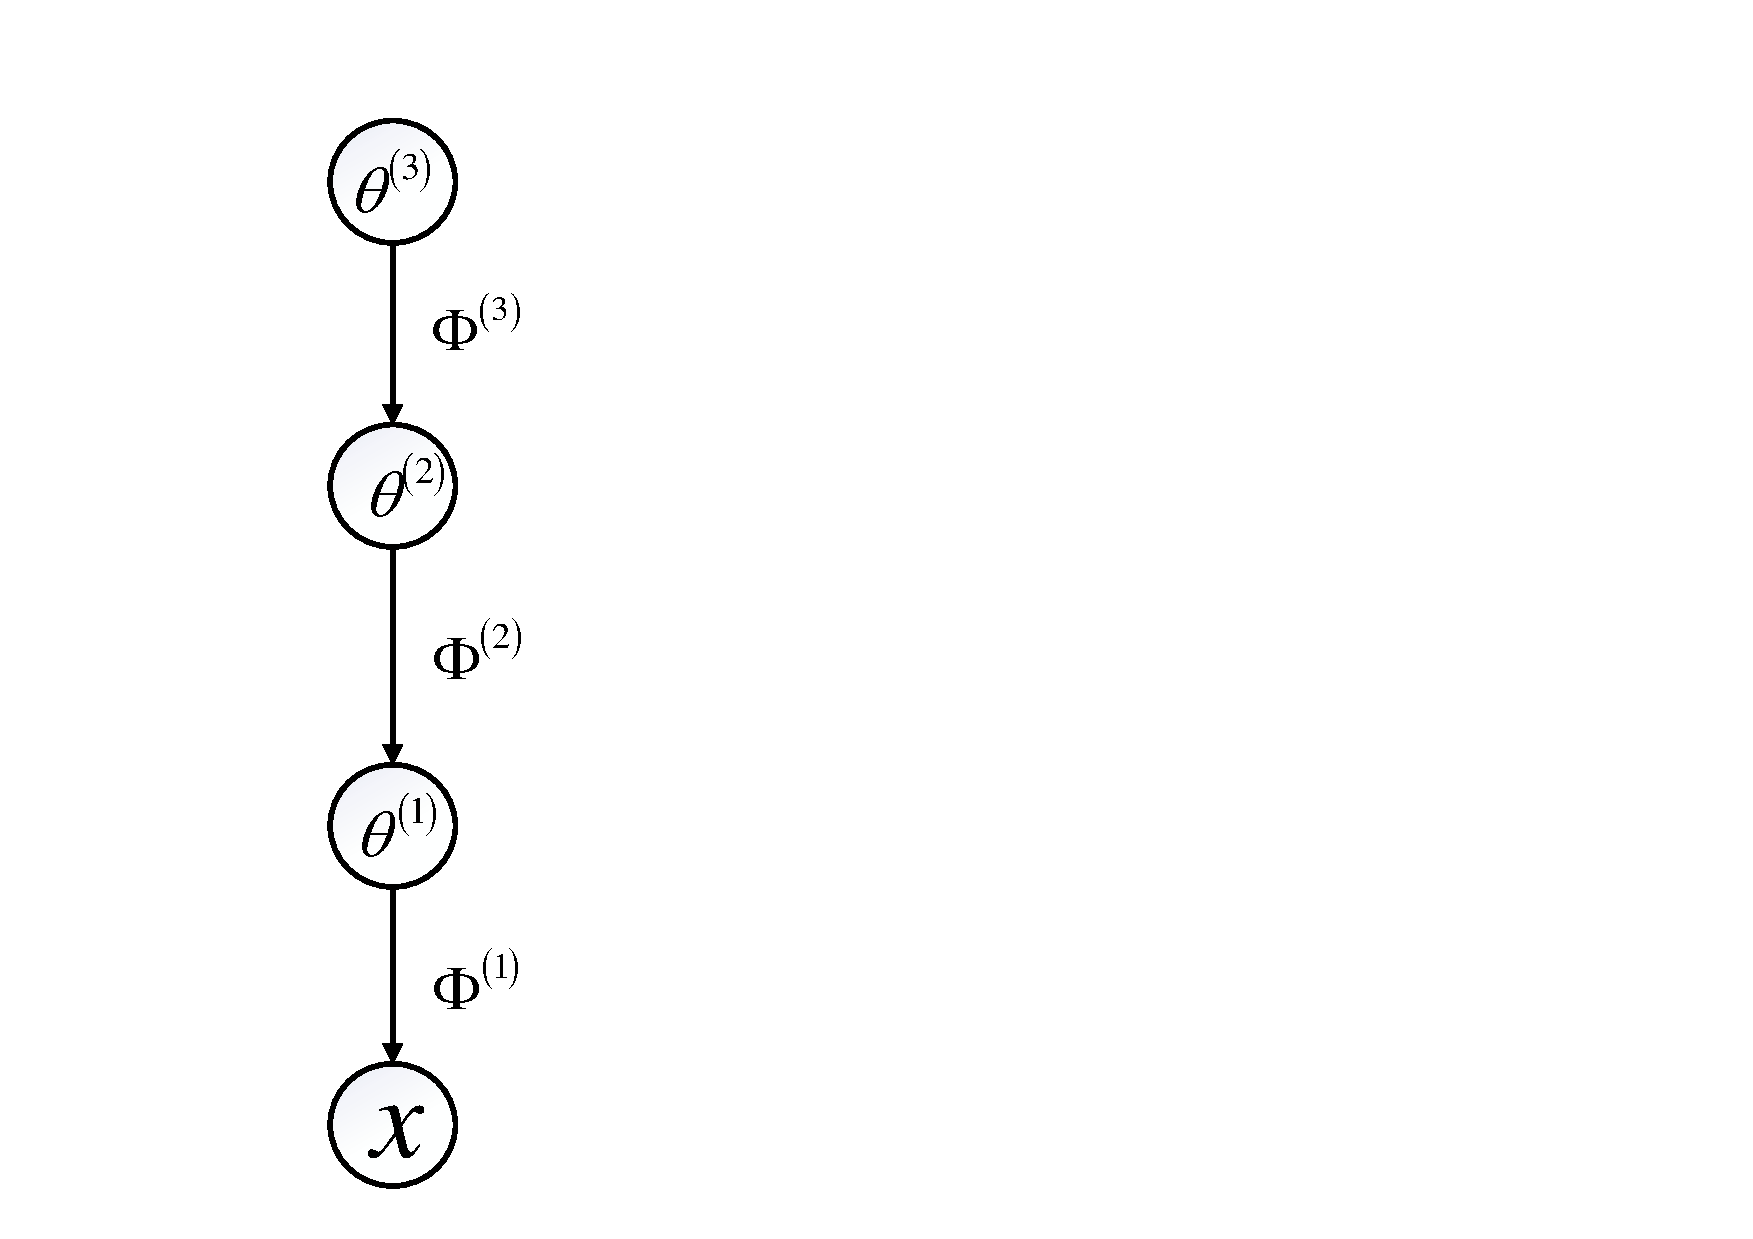
\includegraphics[width=8mm]{figure/figure_generative_model.pdf}
  \label{fig:generate}}
  \quad \quad
  \subfigure[]{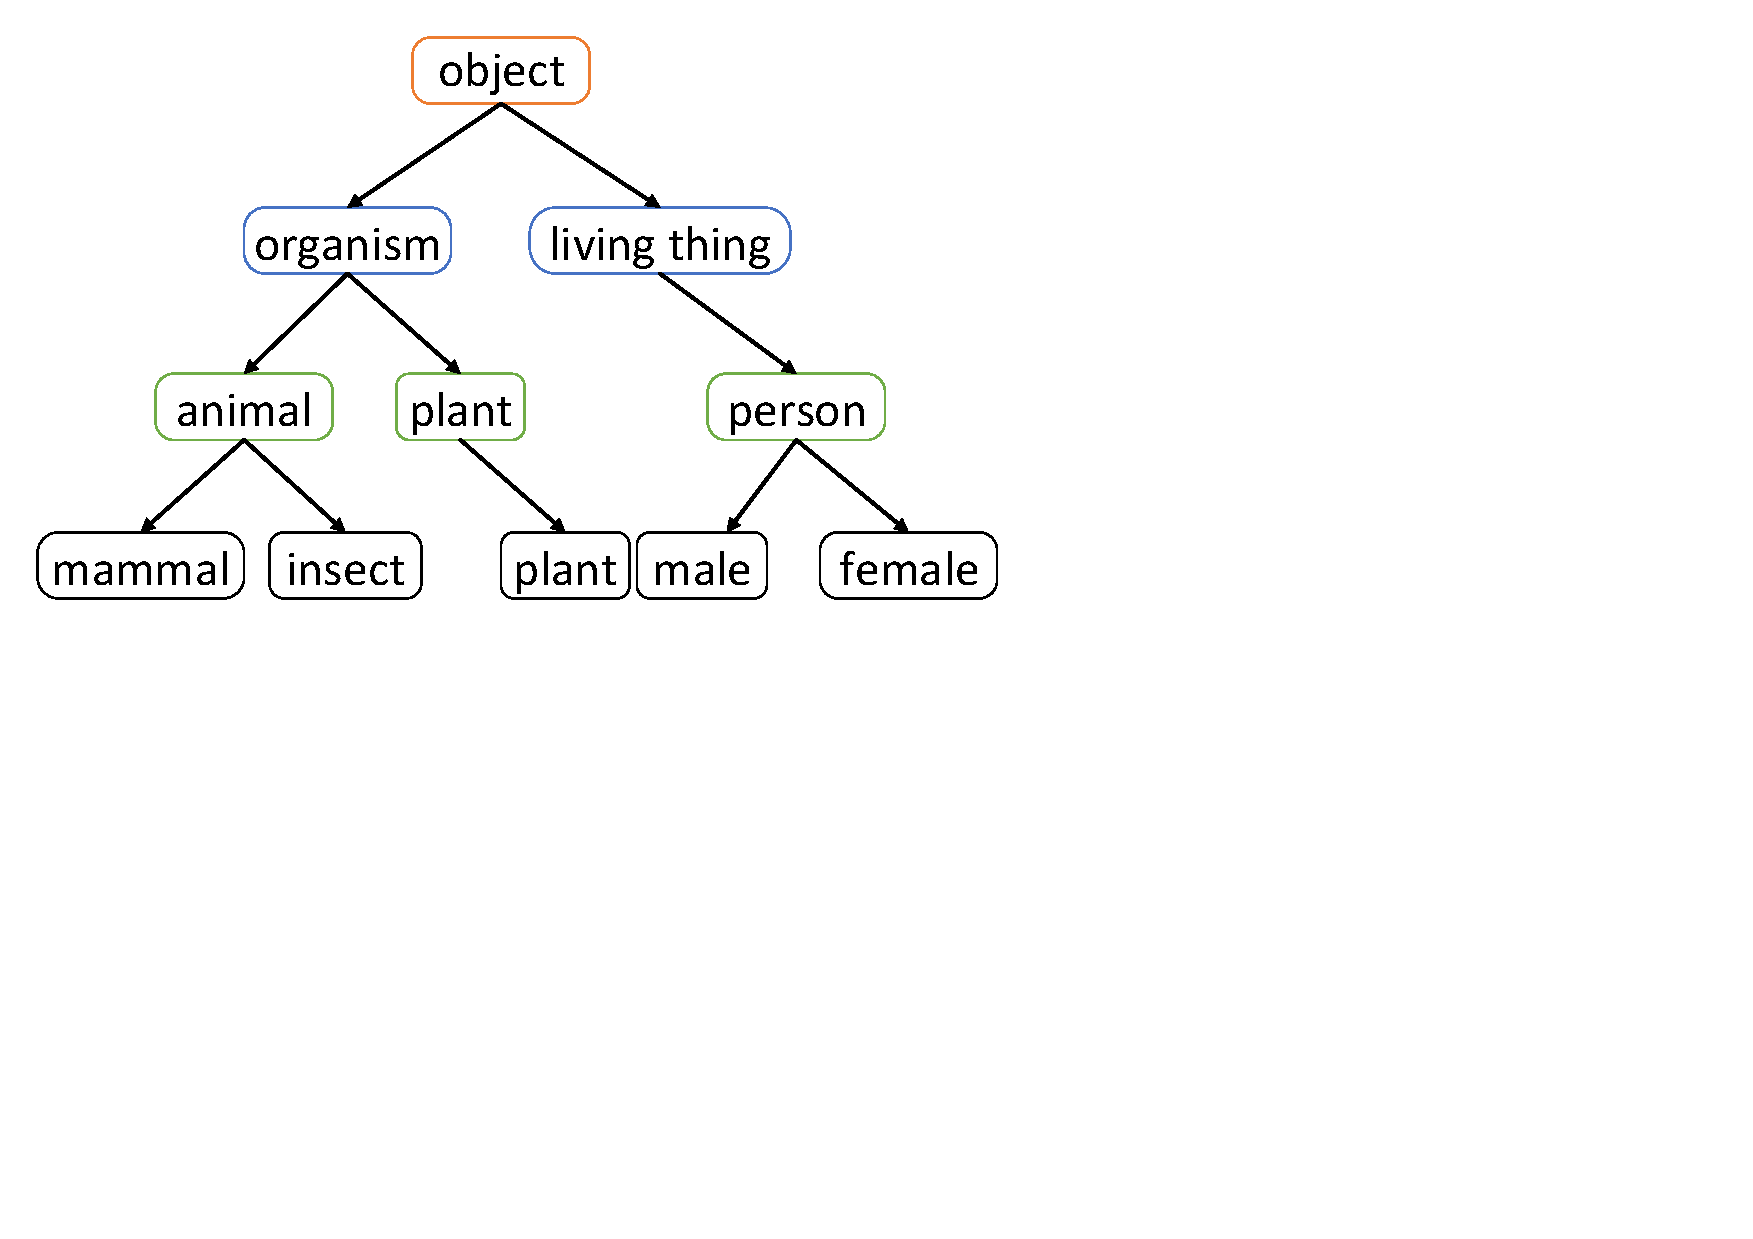
\includegraphics[width=56mm]{figure/figure_TopicTree.pdf}
  \label{fig:wordNet}}
  \quad 
  %\quad \quad \quad
  \subfigure[]{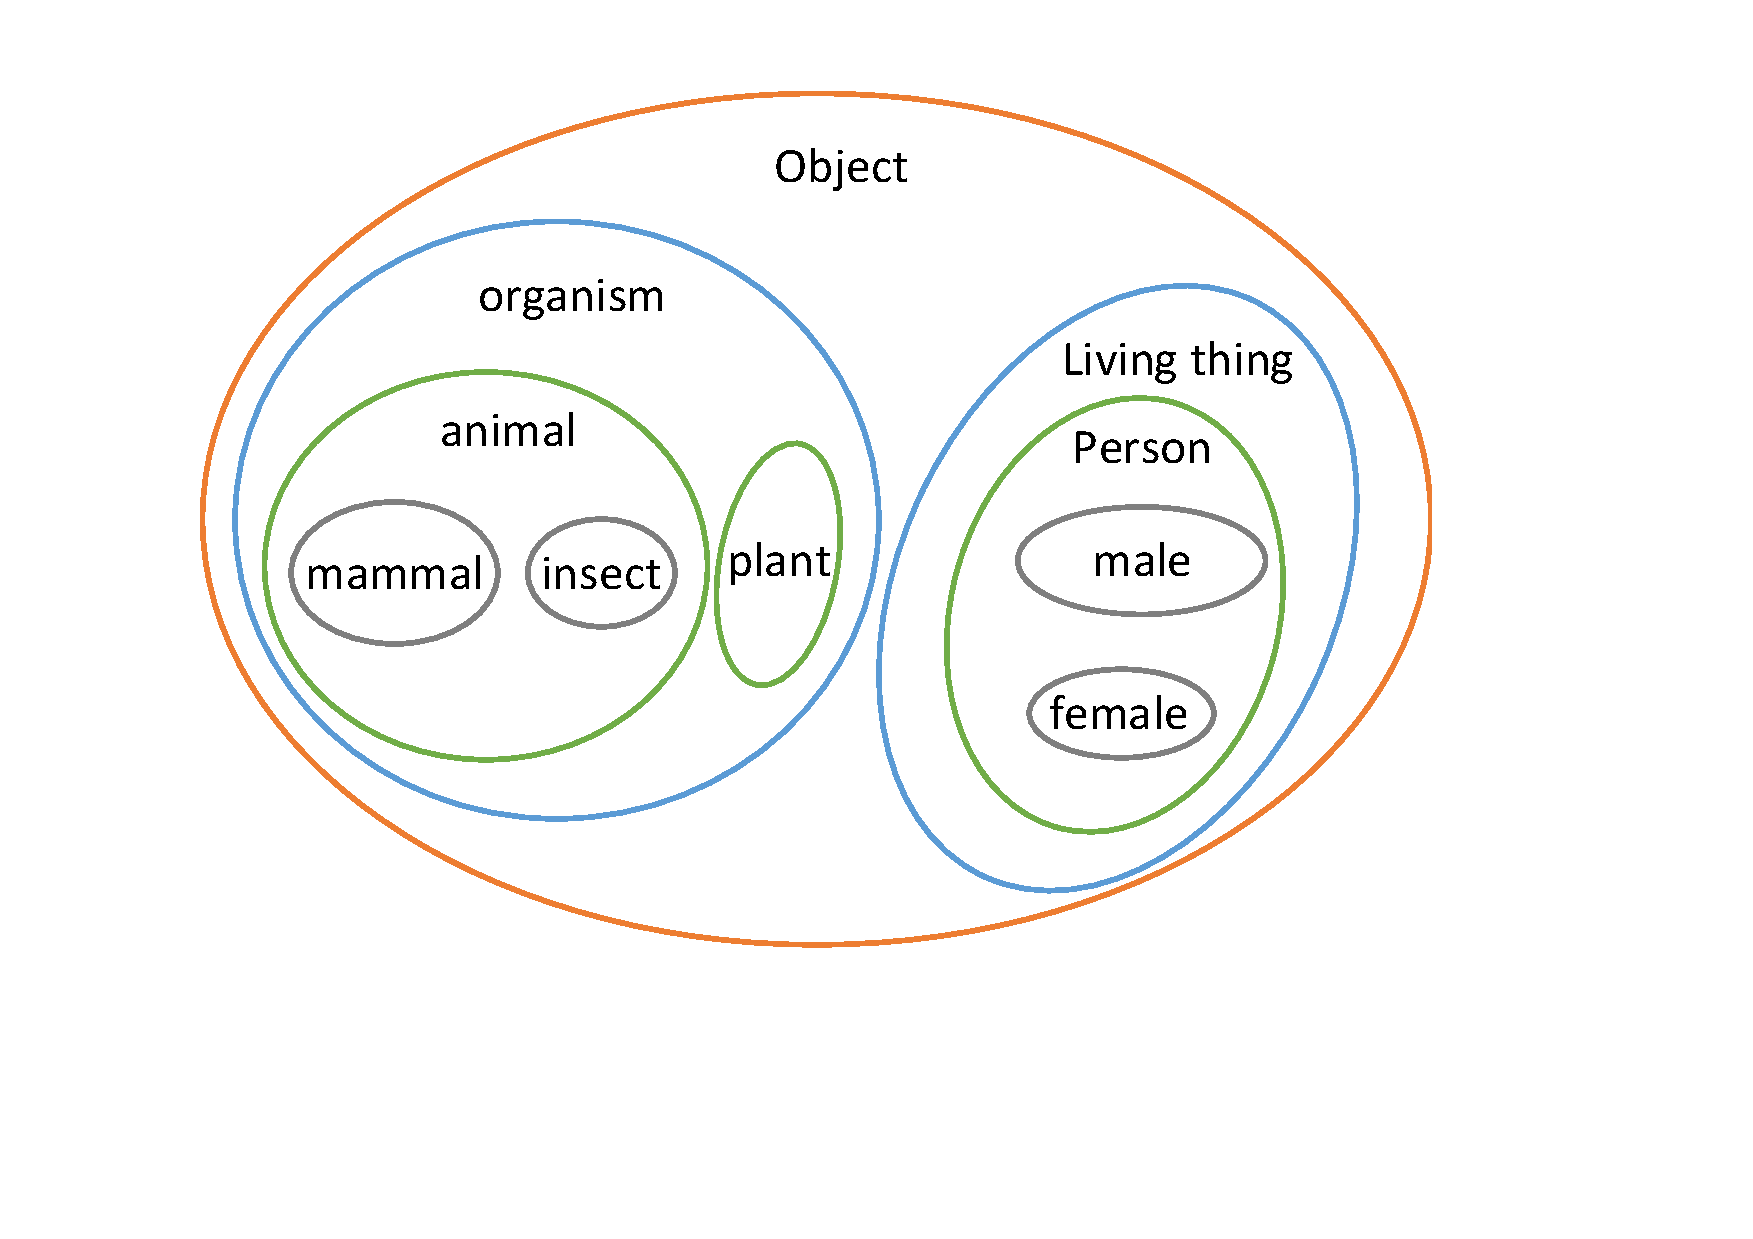
\includegraphics[width=48mm]{figure/figure_WordNet_gaussian_embdding.pdf}
  \label{fig:wordNet_gaussian_embedding}}
  \caption{\small Overviews of (a) generative model of Gaussian SawETM, (b) TopicTree constructed by WordNet, and (c) Density order embeddings where specific entities correspond to concentrated distributions encapsulated in broader distributions of general entities. }
 \label{model}
\end{figure*} 
 %\vspace{-3mm}
\subsection{TopicTree: Semantic graph constructed by prior knowledge}\label{sec:topictree}  
% \begin{algorithm}[tb]
%   \caption{Building TopicTree}
%   \label{alg:example}
% \begin{algorithmic}
%   \STATE Set mini-batch size $m$ and the number of layer $L$
%   \STATE Initialize the encoder parameters $\Omegav $ and decoder parameters $\bm{\Psi}$;
%   \FOR{$iter = 1,2, \cdot \cdot \cdot $} 
%   \STATE Randomly select a mini-batch of $m$ documents to form a subset ${\rm{X}} = {\left\{ {{\xv_i}} \right\}_{1,m}}$;
%   \STATE Dram random noise $\left\{ {\bm{\varepsilon} _i^l} \right\}_{i = 1,l = 1}^{m,L}$ from uniform distribution;
%     \STATE Calculate  $\nabla {}_{\Omegav , {\bm{\Psi}}}L\left( {\Omegav ,{\bm{\Psi}};{\rm{X,}} \left\{ {{\bm{\varepsilon} _i^l}} \right\}_{i = 1,l = 1}^{m,L}} \right)$ according to Eq.~\eqref{ELBO}, and update encoder parameters $\Omegav $ and decoder parameter $\bm{\Psi}$ jointly ;
%   \ENDFOR
% \end{algorithmic}
% \end{algorithm} 
Finding an appropriate way to encode prior knowledge is especially important for realizing the incorporation of prior belief into topic models. Due to the hierarchical structure of deep topic models, correspondingly, we represent prior knowledge in the form of a hierarchical semantic graph and we call it TopicTree. Particularly, in the TopicTree each node is described by a semantic concept and the concepts of nodes at two adjacent layers follow the entailment relations, which results in a bottom-up process of gradual abstraction, as shown in Fig. \ref{fig:wordNet}. Besides, it is worth mentioning that some generic knowledge graphs such as WordNet \cite{miller1995wordnet} provide us a convenient way to build the TopicTree, since the hypernyms or hyponyms of any given word can be easily found in them.  
% which represent the hyperym relation between concepts. Due to the complex of language, there are structure, which not with the structure of hierarchical topic model.  not a tree, because language is complex. For example a ``dog'' is both a type of ``canine'' and a type of ``domestic animal'' which are both synsets in WordNet. Instead of using the full graph structure, we simplify the problem by building a hierarchical tree from the concepts in ImageNet. To build this tree we examine the visual nouns in ImageNet and look at their paths through the WordNet graph to the root node, in this case ``physical object''. Many synsets only have one path through the graph so first we add all of those paths to our tree. Then we iteratively examine the concepts we have left and add the paths that grow the tree by as little as possible. So if a concept has two paths to the root and one path would add three edges to our tree and the other would only add one edge, we choose the shorter path. WordNet can be denoted as a directed graph $\mathcal{G} = \{\mathcal{V} ,\mathcal{E} \}$, where $\mathcal{V}$ denotes the set of concept nodes and $\mathcal{E}$ denotes the set of directed edges. And the directed edge represent the hypeream relationship between concepts, such as . Note that, hierarchical topic model is structured as a tree, and is . TopicTree can be denoted a tree $\mathcal{T} = \{\mathcal{}, \mathcal{} \}$,  we build a hierarchical c . Because language is complex, WordNet \cite{miller1995wordnet} is structured as a directed graph.  For example a ``dog'' is both a type of ``canine'' and a type of ``domestic animal'' which are both synsets in WordNet. 


% Note that, Gaussian distrubution can express asymmetries more naturally than dot product or cosine similarity, which is necessary to represent inclusion or entailment.  imposes a high penalty when there is a region of points $x$ such that the density $f(x)$ is low but $g(x)$ is high. An example of such a regain is the area on the left of $f$ in Figure . This measure penlizes the situation where $f$ is a concentrated distribution relative to $g$; that is, if the distribution $f$ is encompassed by g, then the KL0 yields high penalty. For $d-$dimensional Gaussian $f=N_d()$ and 
\subsection{Partial order: Asymmetric entailment relationship} 
As described in Section \ref{sec:topictree}, 
% Given a TopicTree
we organize prior knowledge into a hierarchical semantic graph so that it can be incorporated into our Gaussian SawETM naturally. Specifically, for a constructed TopicTree with depth $T$, we build a Gaussian SawETM with $T$ latent layers corresponding to it, then we match the topics of each layer in the Gaussian SawETM with the semantic concepts of the corresponding layer in the TopicTree, $i.e.$, each topic has a corresponding semantic concept to describe it. Most significantly, the relationships between semantic concepts in the TopicTree should also be injected
to guide the learning of the topic hierarchy. Since the Gaussian SawETM projects the topics of all layers to a shared embedding space, such a goal can be achieved by imposing constraints on the topic representations in the shared embedding space.
 
Inspired by \citet{vendrov2015order}, the semantic hierarchy (akin to the hypernym relation between words) of the TopicTree can be seen as a special case of the partial order structure. In detail, a partial order over a set of points $X$ is a binary relation $\preceq$ such that for $a,b,c \in X$, the following properties hold: 1) $a \preceq a$ (reflexively); 2) if $a \preceq b$ and $b \preceq a $ then $a=b$ (anti-symmetry); 3) if $a \preceq b$ and $b \preceq c$ then $a \preceq c$ (transitivity). %Thereupon, 
\citet{vendrov2015order} propose learning such asymmetric relationships with order embeddings:  they represent semantic concepts as vectors of non-negative coordinates, and stipulate that smaller coordinates imply higher position in the partial order and correspond to a more general concept. For example, the following expression defines an ordered pair $(x,y)$ of vectors in $\mathbb{R}_+ ^N$:
\begin{equation}\label{eq:order_ebmd}
\small
\begin{split}
\xv \preceq \yv \text{ if and only if} \bigwedge_{i = 1}^N \xv_i \geq \yv_i . 
\end{split}
\end{equation}
Since the order embedding condition defined by Eq. \eqref{eq:order_ebmd} is too restrictive to satisfy by imposing a hard constraint, \citet{vendrov2015order} relax the condition and turn to seek an approximate order-embedding. In particular, for an ordered pair of points, they apply a penalty that is formulated as:
\begin{align}\label{eq:order_penalty}
\Ev(\xv,\yv) = {\|\max (0,\yv-\xv)\|}^2.
\end{align}
Note that this imposes a strong prior on the embeddings, which could encourage the learned relations to satisfy the partial order properties of transitivity and antisymmetry.

Although Gaussian-distributed embeddings are used to represent topics in our Gaussian SawETM, we find that they are also natural at capturing the partial order structure (or the semantic hierarchy of the TopicTree) \cite{das2015gaussian, athiwaratkun2018hierarchical}. For instance, for two topics following the hypernym relation, their Gaussian-distributed embeddings $\bm{\alpha}_i$ and $\bm{\alpha}_j$ form an ordered pair. Assuming that $\bm{\alpha}_i$ represents the specific topic and $\bm{\alpha}_j$ represents the general one, then we have $\bm{\alpha}_i \preceq \bm{\alpha}_j$, meanwhile we expect that $\bm{\alpha}_j$ corresponds to a broad distribution that encompasses $\bm{\alpha}_i$. To meet this expectation, the KL divergence between $\bm{\alpha}_i$ and $\bm{\alpha}_j$ provides us a ready-made tool:
%\begin{small}
% \mz{use resize box rather small font}
\begin{equation} \label{KL}
\small
\begin{split}
\mbox{\Ev}^{\text{(a)}} \left( {{\bm{\alpha} _i},{\bm{\alpha} _j}} \right) = {D_{KL}}\left( {{\Nv_i}\parallel {\Nv_j}} \right) = \int_{\bm{x} \in {\mathbb{R}^n}} {N\left( {\bm{x};{\bm{\mu} _i},{\bm{\Sigma} _i}} \right)\log \left( {{{N\left( {\bm{x};{\bm{\mu} _i},{\bm{\Sigma} _i}} \right)} \mathord{\left/
 {\vphantom {{N\left( {\bm{x};{\bm{\mu} _i},{\bm{\Sigma} _i}} \right)} {N\left( {\bm{x};{\bm{\mu} _j},{\bm{\Sigma} _j}} \right)}}} \right.
 \kern-\nulldelimiterspace} {N\left( {\bm{x};{\bm{\mu} _j},{\bm{\Sigma} _j}} \right)}}} \right)d\bm{x}} \notag \\
  = \frac{1}{2}\left( {{\text{tr}}\left( {\bm{\Sigma} _j^{ - 1}{\bm{\Sigma} _i}} \right) + {{\left( {{\bm{\mu} _i} - {\bm{\mu} _j}} \right)}^{\text{T}}}\bm{\Sigma} _j^{ - 1}\left( {{\bm{\mu} _i} - {\bm{\mu} _j}} \right) - d + \log \left( {{{\det \left( {{\bm{\Sigma} _j}} \right)} \mathord{\left/
 {\vphantom {{\det \left( {{\bm{\Sigma} _j}} \right)} {\det \left( {{\bm{\Sigma} _i}} \right)}}} \right.
 \kern-\nulldelimiterspace} {\det \left( {{\bm{\Sigma} _i}} \right)}}} \right)} \right)
\end{split}
\end{equation}
%\end{small}
However, using $\mbox{E}^{\text{(a)}}({\bm{\alpha}_i},{\bm{\alpha}_j})$ directly as a penalty for violating the partial order is undesirable. Since the KL divergence has a property that $\mbox{E}^{\text{(a)}}({\bm{\alpha}_i},{\bm{\alpha}_j})=0$ if and only if $\bm{\alpha}_i=\bm{\alpha}_j$, which means the penalty is zero only if $\bm{\alpha}_i=\bm{\alpha}_j$, but we expect the penalty should also be zero when $\bm{\alpha}_i \neq \bm{\alpha}_j$ and $\bm{\alpha}_i \preceq \bm{\alpha}_j$. For this reason, following \citet{athiwaratkun2018hierarchical}, we consider using a thresholded divergence as our penalty for order violation:
\begin{equation}\label{eq:distance}
\small
\begin{split}
{d_\gamma }\left( {\bm{\alpha}_i,\bm{\alpha}_j} \right) = \max \left( {0,{\mbox{\Ev} ^{\text{(a)}}({\bm{\alpha}_i},{\bm{\alpha} _j})  - \gamma}} \right).
\end{split}
\end{equation}
So this penalty can be zero if $\bm{\alpha}_i$ is properly encapsulated in $\bm{\alpha}_j$. Nevertheless, note that we no longer have the strict partial order with such a penalty. In other words, the transitivity and anti-symmetry are not guaranteed. Therefore, actually our learned relations also respect an approximate order structure. 
%For example, if $\bm{\alpha}_i \preceq \bm{\alpha}_j$ and $\bm{\alpha}_j \preceq \bm{\alpha}_k$, our embeddings would yeild ${d_\gamma}(\bm{\alpha}_i,\bm{\alpha}_j) = 0$ and ${d_\gamma}(\bm{\alpha}_j,\bm{\alpha}_k) = 0$, but it is not necessarily the case that since $D_KL$; ${d_\gamma}(\bm{\alpha}_i,\bm{\alpha}_k) = 0$
%According to Eq. (\ref{eq:distance}), when $\mbox{E} ^{\text{(a)}}$ is small enough ${d_\gamma}(\alpha_i,\alpha_j) = 0$ \iff $\alpha_i \preceq \alpha_j$ %\Longrightarrow  %is small enough, ac However, this penalty is difficult to evaluate for most distributions, including
%Gaussians. Instead, we use simple penalty functions based on asymmetric divergence measures between probability densities. Divergence measures $D(\cdotv\parallel\cdotv)$ have a property that $D(f\parallelg)=0$ if and
%only if $f = g$. Using $D(\cdotv\parallel\cdotv)$ to represent order violation is undesirable since the penalty should be 0
%if f 6= g but f ? g. Therefore, we propose using a thresholded divergence


%which can be zero if f is properly encapsulated in g .
% the order relation of this  

% a Gaussian distribution 


% That is, a density $f$ is more specific than a density $g$ if $f$ is encompassed in $g$. The degree of encapulation can vary, which gives rise to multiple order relations. We define an order relation $\preceq _\eta$ for $\eta  \geqslant 0$ where $\eta$ indicates the degree of encapsulation required for one distribution to entail another. More precisely, for distribution $f$ and $g$,
% \begin{align}\label{eq:density_order}
% f{ \preceq _\eta } g \Leftrightarrow \left\{ {x:f\left( x \right) > \eta } \right\} \subseteq \left\{ {x:g\left( x \right) > \eta } \right\},
% \end{align}
% Note that ${x:f\left( x \right) > \eta }$ is a set where the density $f$ is greater than the threshold $\eta$. The relation in says in Equation ~\ref{eq:density_order} that $f$ entails $g$ if and only if the set of $g$ contains that of $f$. 

% This concept has applications in natural data such lexical entailment. For words $a$ and $b$, $a \preceq b$ means that every instance of $a$ is an instance of $b$, or we can say that $a$ entails $b$. we also say that $(a, b)$ has a $hypernym$ relationship where $a$ is a hyponym of $b$ and $b$ us a hyprtnym of $a$. This relationship is asymmetric since $a \preceq b$ does not necessarity imply $(b \preceq a)$. For instance,  $aircraft \preceq vehicle$ but it is not true that $vehicle \preceq aircraft$. 

% The prior semantic is the TopicTree, which is proposed in Section ~\ref{sec:topictree}, this structure is defined as partial order structure in  \cite{vendrov2015order}. And  \cite{vendrov2015order, athiwaratkun2018hierarchical} introduce methods to capture the hierarchical structure in the embedding space. 
% An order-embedding is a function $f: (X,\preceq ) (Y, \preceq)$ where if and only if .  \cite{vendrov2015order} propose to learn the embedding  $f$ on where all coordinates are non-negative. 
% A partial order on probability densities can be obtained by the notion of encapsulation.
%A symmetric similarity function is not enough to relflect the hypernomy/hyponymy relation between topics. Fortunately, with Gaussian-distributed embeddings to represent topics, the Kullback-Leibler(KL) divergence provides a natural way to express the asymmetric similarity such as the inclusions and entailments between topics . Specially, the KL divergence of two Gaussian distributions $\alpha _i$ and $\alpha _j$ can be expressed as:

%where ${\mu _i}$ is the mean and ${\sum\nolimits_i}$ the covariance matrix of the Gaussian distribution. Note that, KL divergence is natural energy function for representing entailment between concepts: a low KL divergence from $\alpha _i$ to $\alpha _j$ indicates that we can encode $\alpha _j$ easily as $\alpha _i$, implying that $\alpha _j$ entails $\alpha _i$. This can be more intuitively visualized and interpreted as a soft form of inclusion between the level sets of ellipsoids generated by the two Guassians - if there is a relatively high expected log-likelihood ratio (negative KL), then most of the mass of $y$ lies inside $x$. 

\subsection{Objective: ELBO with a prior regularity}
Essentially, TopicNet is a topic model, so the ELBO still plays a leading role in the training objective. At the same time, a regularization term is also necessary for injecting hierarchical prior knowledge to guide the topic discovery. Therefore, the final objective of TopicNet can be written as:
\begin{align}\label{eq:topicnet}
\Lv _{\text{TopicNet}} = \Lv _{\text{ELBO}} + \beta  \Lv _{\text{prior}},
\end{align}
where $\beta$ is a hyper-parameter used to balance the impact of these two terms. Particularly, for the ELBO term $L _{\text{ELBO}}$, it is the same as defined by Eq.~(\ref{ELBO}). As for the regularization term $L _{\text{prior}}$, we cannot only %consider  %
constrain topics that follow the hypernym relation between two adjacent layers, but the topics that do not follow the hypernym relation should also be considered. This is consistent with the notion of positive and negative sample pairs in contrastive learning. Based on this idea, we use a max-margin loss to encourage the largest penalty between positive sample pairs to be below the smallest penalty between negative sample pairs, which is defined as:
%Based on the idea of contrastive learning, positive and negative examples
%Inspired by the loss function in previous work \cite{vilnis2014word, athiwaratkun2018hierarchical}, with the distance in Eq.~\eqref{eq:distance}, we could use a max-margin loss to capture the hypernym relation between the parent nodes with its children nodes, which encourages positive examples to have zero penalty, and negative examples to have penalty greater than a margin. Specially, for a parent node topic $\mathtt{j ^{(t+1)}}$ at $\mathtt{(t+1) ^{th}}$ layer, the children nodes  of this topic $\mathtt{j ^{(t+1)}}$ at $\mathtt{t ^{th}}$ layer can form a set as $\mathtt{D _j ^{(t+1)}}$, to capture the structure between the parent node with its children node, we defined the loss function as:
\begin{align}\label{eq:rank_loss}
\Lv _{j} ^{(t+1)} = \max(0, m - \max {\left\{ {d_\gamma \left( {i,j} \right)} \right\}_{i \in D}} + \min {\left\{ {d_\gamma \left( {i,j} \right)} \right\}_{i \notin D}}) .
\end{align}
This represents the penalty for the $j^{th}$ topic at ${(t+1)^{th}}$ layer, and $D$ is the set of hyponym topics of topic $j$. For $i \in D$, $(i, j)$ forms a positive pair, for $i \notin D$, $(i, j)$ forms a negative pair. Parameter $m$ is the margin that determines the degree to which the positive and negative pairs are separated. Considering the penalties for all topics in each layer, we obtain the prior regularization term.
%Specially, for a parent node topic $\mathtt{j ^{(t+1)}}$ at $\mathtt{(t+1) ^{th}}$ layer, the children nodes  of this topic $\mathtt{j ^{(t+1)}}$ at $\mathtt{t ^{th}}$ layer can form a set as $\mathtt{D _j ^{(t+1)}}$
%+ \max \left\{ {0,m - {{\left\{ {d\left( {i,j} \right)} \right\}}_{i \notin D}}} \right\}
%where the first term $\max {\left\{ {d_\gamma \left( {i,j} \right)} \right\}_{i \in D}}$ is to \mz{????}, the second term $\min {\left\{ {d_\gamma \left( {i,j} \right)} \right\}_{i \notin D}}$ is to , and the final optimized object is to let the most with the max-margin,.
%And then summing all the loss of parent node in the TopicTree, can result in the prior knowledge supervised loss as:
\begin{align}\label{eq:prior_loss}
\Lv _{\text{prior}} = \sum\nolimits_{t = 0}^{T - 1} {\sum\nolimits_{j = 0}^{{K^{\left( {t + 1} \right)}}} {\Lv_j^{\left( {t + 1} \right)}} }.
\end{align}
% To jointly learn the topic model and density order embeddings, inspired by the loss function of  , we propose a prior knowledge supervised loss function. 
% \begin{align}\label{eq:prior_loss}
% L _{\text{prior} = 0 
% \end{align}
%To balance the impact of ELBO and supervisory losses, we introduce a hyper-parameter $\beta$ into the prior loss, and the TopicNet loss can be expressed as:
With the final objective, TopicNet learns the topics influenced by both the word co-occurrence information and prior semantic knowledge, thus discovering more interpretable topics. Note that, in our experiments, the hyper-parameters are set as $m = 10.0$ and $\beta =1.0$.
% the evidence lowerbound (ELBO) of data log-likelihood $\log p(\Xmat, \Amat)$, which can be expressed as
\subsection{Model Properties} 
In this part, we recap several good properties of TopicNet: Uncertainty, Interpretability, and Flexibility.

\paragraph{Effectiveness of Gaussian-distributed embeddings:} Mapping a topic to a distribution instead of a vector brings many advantages, including: on  one hand, better capturing uncertainty about a representation, where the mean indicates the semantics of a topic and the covariance matrix reflects its level of abstraction; on the other hand, expressing asymmetric relationships more naturally than point vectors, which is beneficial to modeling the partial order structure of semantic hierarchy \cite{vilnis2014word,athiwaratkun2018hierarchical}.
\paragraph{Hierarchical interpretable topics:} In conventional hierarchical topic models, the semantics of a topic is reflected by its distributed words, and we have to summarize a semantically coherent concept manually by post-hoc visualization. In some cases, the topic is too abstract to get a semantically coherent concept, which makes it hard to interpret. Such cases are common in deeper hidden layers. While in TopicNet, we know in advance what semantic concept a certain topic corresponds to, since it is encoded from prior knowledge and used to guide the topic discovery process of the model as a kind of supervision information. Therefore, once the model is trained, the words distributed under each topic are semantically related to the concept that describes it, as shown in Fig.~\ref{fig:hier_structure}. From this perspective, our TopicNet has better interpretability.
% discover interpretable topics by using the structure to guided topic learning. Note that, it is 
\paragraph{Flexibility to incorporate prior belief:} Traditional topic models learn topics only by capturing word co-occurrence information from data, which do not consider the possible prior domain knowledge ($e.g.$, Knowledge Graph like WordNet \cite{fellbaum2010wordnet}). However, TopicNet provides a flexible framework to incorporate the structured prior knowledge into hierarchical topic models. 

\section{TopNet Integration: Neural Topic-Driven Story Generation} \label{sec:topnet_integration}

Building upon the semantic graph-guided topic discovery capabilities of TopicNet, we introduce an innovative extension that integrates TopNet's neural topic modeling approach for coherent story generation. This integration represents a paradigm shift from pure topic understanding to a unified framework that bridges semantic comprehension with narrative generation.

\subsection{Motivation and Innovation}

While TopicNet excels at discovering interpretable topic hierarchies guided by semantic graphs, many real-world applications require not just understanding but also generation capabilities. For instance, in news analysis, journalists and content creators need tools that can both understand the thematic structure of articles and generate coherent narratives based on discovered topics. This dual requirement motivates our integration of TopNet's story generation framework with TopicNet's semantic understanding.

The key innovation lies in our cross-modal architecture that seamlessly connects topic discovery with story generation through shared Gaussian embeddings and hierarchical attention mechanisms. Unlike previous approaches that treat understanding and generation as separate tasks, our unified framework enables topic-guided narrative synthesis while maintaining semantic coherence with the discovered topic hierarchy.

\subsection{TopNet Topic Generator Integration}

We integrate TopNet's variational topic modeling approach by extending the Gaussian SawETM with story generation capabilities. The TopNet topic generator maps short text inputs to topic distributions using variational inference, which we align with TopicNet's semantic graph constraints:

\begin{equation} \label{topnet_generator}
\begin{split}
& p(\bm{z}|\bm{x}) = \mathcal{N}(\bm{\mu}_\phi(\bm{x}), \bm{\sigma}_\phi^2(\bm{x})) \\
& p(\bm{w}|\bm{z}) = \text{Cat}(\text{softmax}(\bm{W}_\theta \bm{z})) \\
& \text{subject to: } \mathcal{L}_{\text{semantic}}(\bm{z}, \mathcal{G}) < \gamma
\end{split}
\end{equation}

where $\bm{z}$ represents the topic distribution, $\bm{x}$ is the input text, $\bm{w}$ are skeleton words for story generation, and $\mathcal{G}$ represents the semantic graph constraints from TopicNet. The semantic constraint $\mathcal{L}_{\text{semantic}}$ ensures that generated topic distributions respect the hierarchical structure defined by the semantic graph.

\subsection{Hierarchical Story Generation Framework}

Our hierarchical story generator takes the topic distributions from the integrated topic generator and produces coherent long-form narratives through a novel skeleton-word-guided approach:

\begin{equation} \label{story_generation}
\begin{split}
& \bm{s}_t = \text{LSTM}(\bm{h}_{t-1}, [\bm{e}(\bm{w}_t); \bm{z}_t]) \\
& p(\bm{y}_t|\bm{s}_t, \bm{z}_t) = \text{softmax}(\bm{W}_{\text{gen}} \bm{s}_t + \bm{W}_{\text{topic}} \bm{z}_t) \\
& \text{Attention: } \bm{a}_t = \text{softmax}(\bm{W}_{\text{attn}} \tanh(\bm{W}_{\text{topic}} \bm{z}_t + \bm{W}_{\text{story}} \bm{s}_t))
\end{split}
\end{equation}

where $\bm{s}_t$ is the story state at time $t$, $\bm{w}_t$ are skeleton words, $\bm{z}_t$ is the topic context, and $\bm{a}_t$ provides cross-modal attention between topics and story generation.

\subsection{Cross-Modal Attention Mechanism}

A critical innovation in our framework is the cross-modal attention mechanism that aligns topic discovery with story generation. This mechanism ensures that generated stories maintain semantic consistency with the discovered topic hierarchy:

\begin{equation} \label{cross_modal_attention}
\begin{split}
& \bm{Q} = \bm{W}_Q \bm{H}_{\text{topics}}, \quad \bm{K} = \bm{W}_K \bm{H}_{\text{story}}, \quad \bm{V} = \bm{W}_V \bm{H}_{\text{story}} \\
& \text{Attention}(\bm{Q}, \bm{K}, \bm{V}) = \text{softmax}\left(\frac{\bm{Q}\bm{K}^T}{\sqrt{d_k}}\right) \bm{V} \\
& \bm{H}_{\text{aligned}} = \text{Attention}(\bm{Q}, \bm{K}, \bm{V}) + \bm{H}_{\text{topics}}
\end{split}
\end{equation}

This attention mechanism enables bidirectional information flow between topic understanding and story generation, ensuring that generated narratives are grounded in the semantic topic hierarchy while maintaining narrative coherence.

\subsection{Multi-Task Learning Objective}

The unified TopicNet-TopNet framework is trained using a multi-task objective that combines topic modeling, story generation, and semantic consistency:

\begin{equation} \label{unified_objective}
\begin{split}
\mathcal{L}_{\text{total}} &= \mathcal{L}_{\text{ELBO}} + \lambda_1 \mathcal{L}_{\text{story}} + \lambda_2 \mathcal{L}_{\text{semantic}} + \lambda_3 \mathcal{L}_{\text{alignment}} \\
\mathcal{L}_{\text{story}} &= -\sum_{t=1}^T \log p(\bm{y}_t | \bm{y}_{<t}, \bm{z}) \\
\mathcal{L}_{\text{alignment}} &= \|\bm{H}_{\text{topics}} - \bm{H}_{\text{aligned}}\|_2^2
\end{split}
\end{equation}

where $\mathcal{L}_{\text{ELBO}}$ is the evidence lower bound from TopicNet, $\mathcal{L}_{\text{story}}$ is the story generation loss, $\mathcal{L}_{\text{semantic}}$ enforces semantic graph constraints, and $\mathcal{L}_{\text{alignment}}$ ensures cross-modal consistency. 
% \subsection{Model Properties}
% SawETM inherits the good properties of both deep topic model and Gaussian embeddings, as described below.
% \paragraph{Words and Topics at the same semantic space:} Sawtooch connection can couple the d , and map the words and topics in the same semantic space.  \cite{duan2021sawtooth}. 
% \paragraph{Interpretable:} 
% We evaluate the proposed model by comparing it with several recent advances including Bayesian generative models and neural topic models. The experiments were conducted on  on several benchmark text datasets including both regular and big corpus. We report perplexity, topic quality, and two document cluster metrics. We also qualitatively analyze the learned word and topic embedding, and topic hierarchies.
% \begin{figure*}[!ht]
% \vspace{-5mm}
% \centering
% \subfigure[20NG]{
% 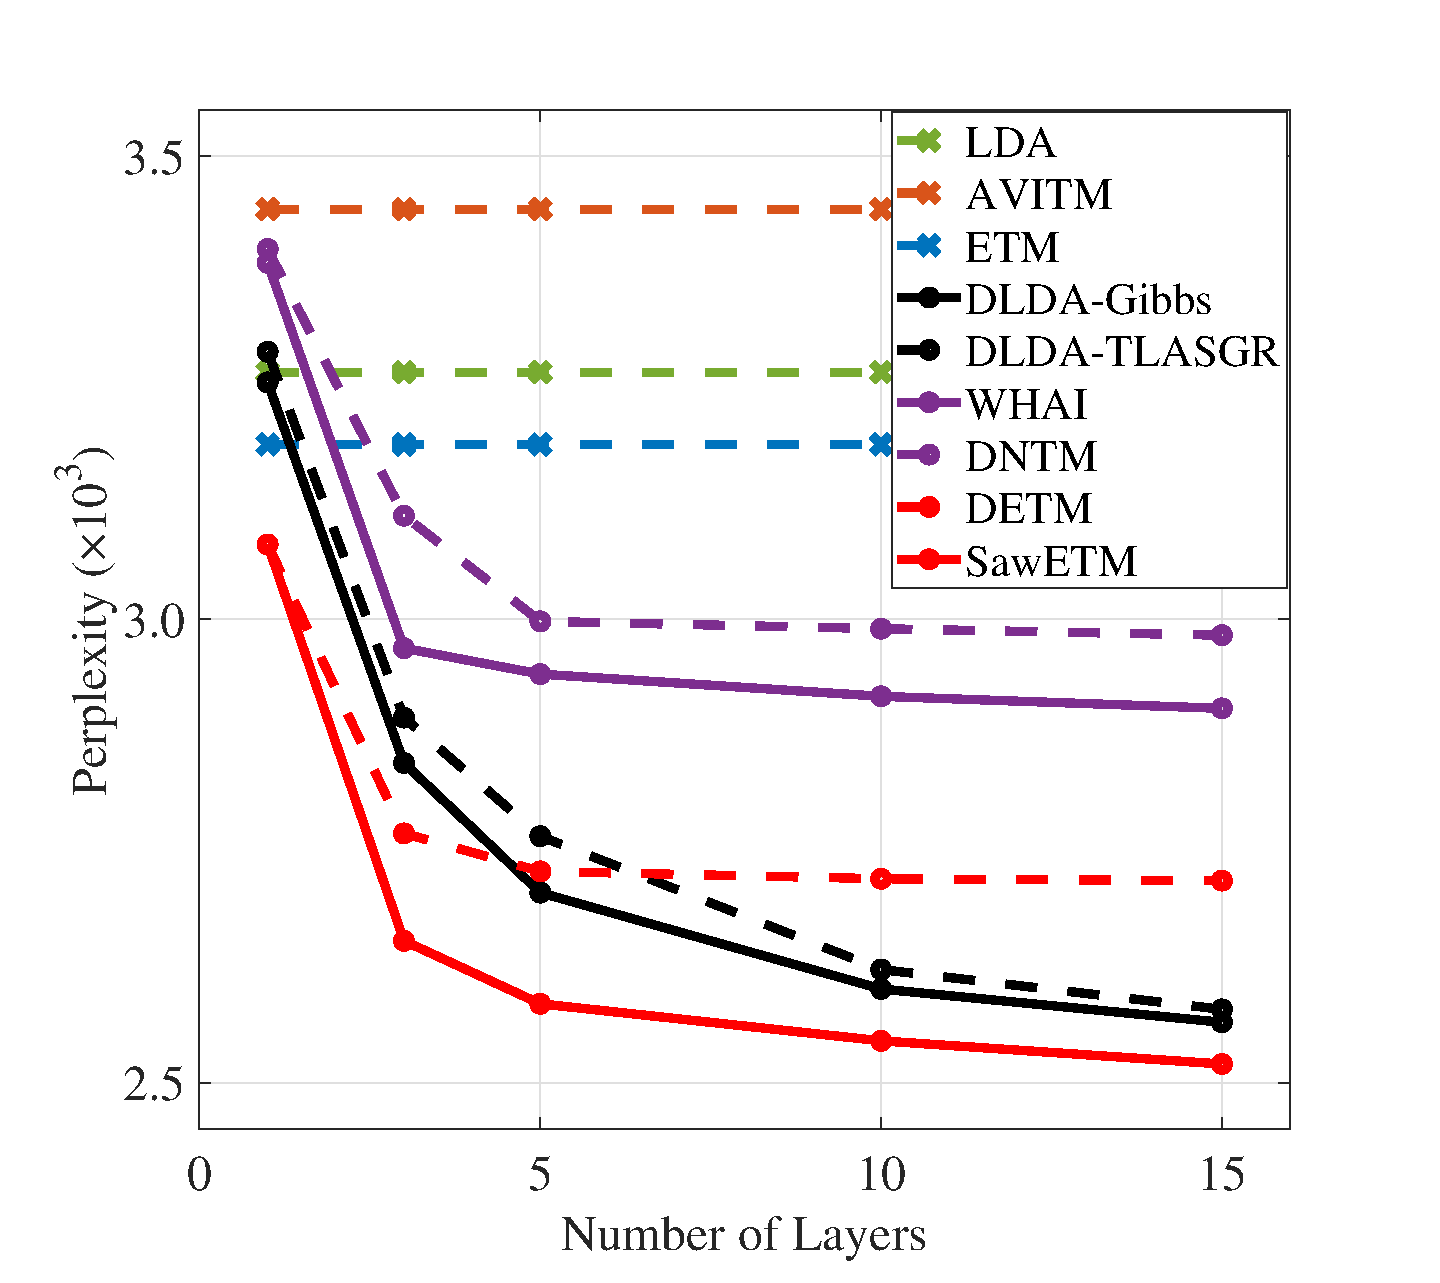
\includegraphics[width=0.31\linewidth]{ppl_result/20ng_ppl.eps}
% } \hspace{-5mm}
% \quad 
% \subfigure[RCV1]{
% 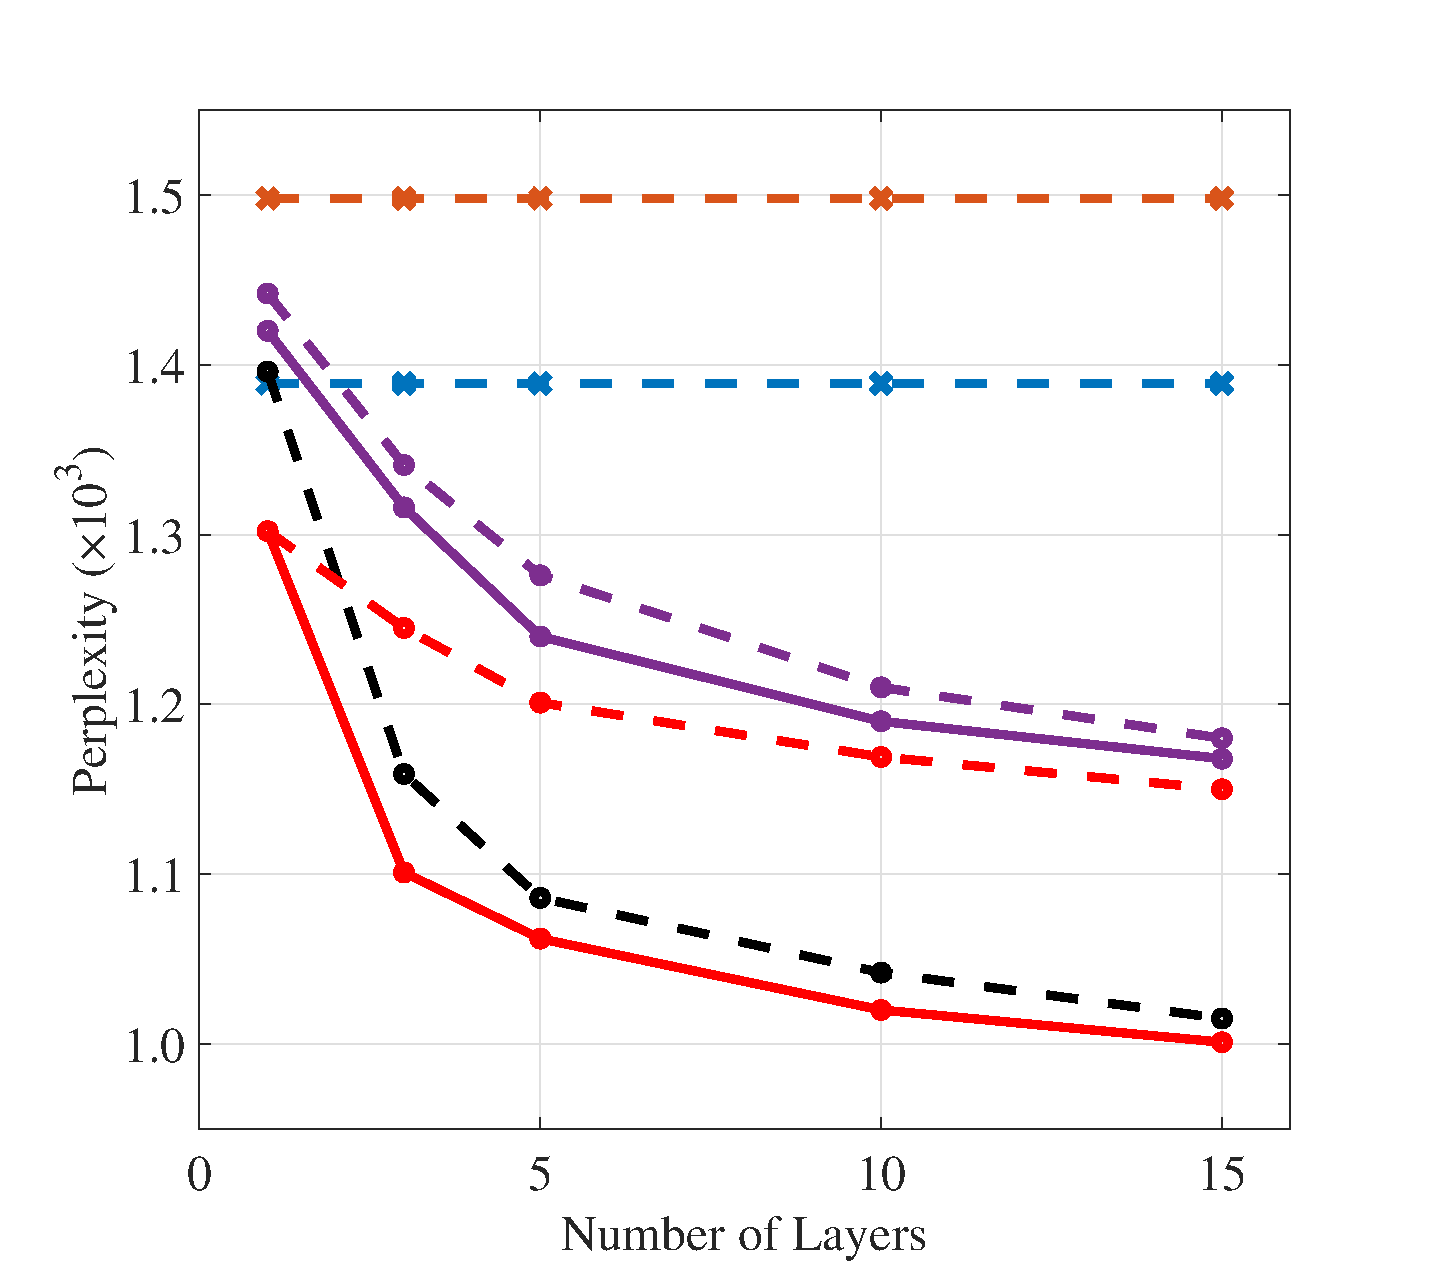
\includegraphics[width=0.31\linewidth]{ppl_result/rcv1_ppl.eps}
% } \hspace{-5mm}
% \quad 
% \subfigure[PG19]{
% 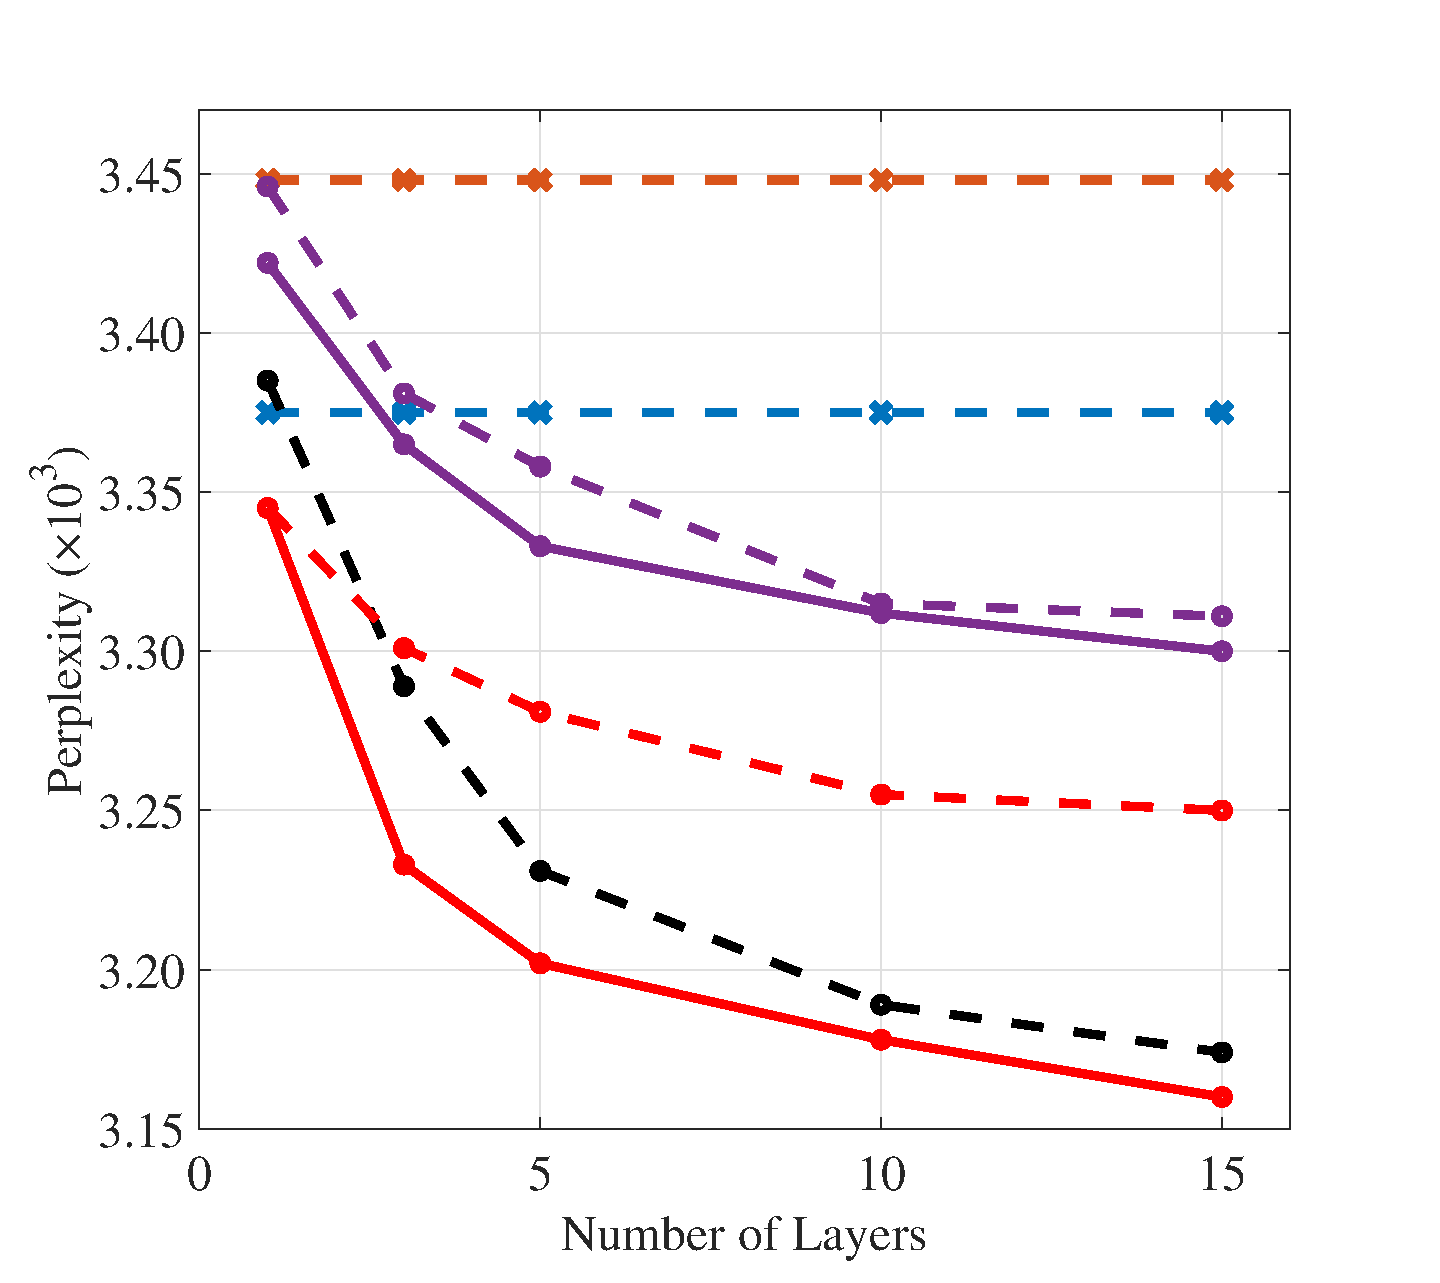
\includegraphics[width=0.31\linewidth]{ppl_result/PG-19.eps}
% }\vspace{-2mm}
% \quad 
% \subfigure[20NG]{
% 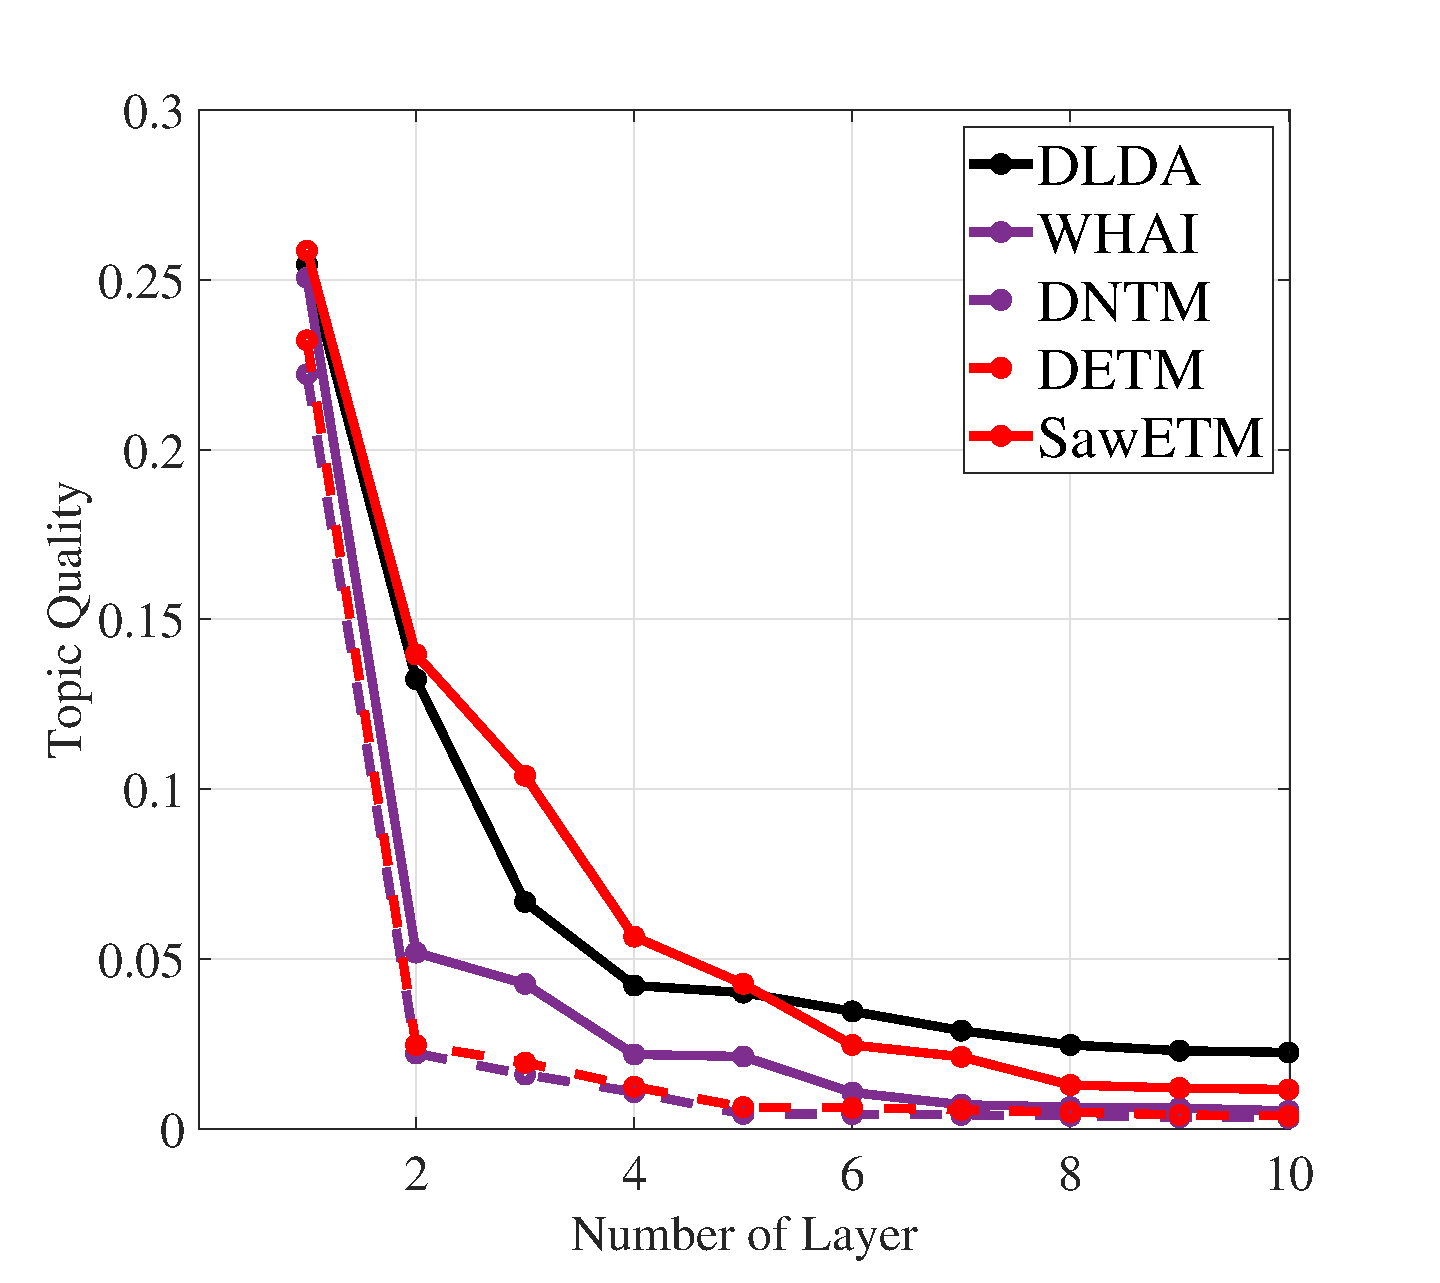
\includegraphics[width=0.31\linewidth]{quality_result/20ng_quality.eps}
% } \hspace{-5mm}
% \quad 
% \subfigure[RCV1]{
% 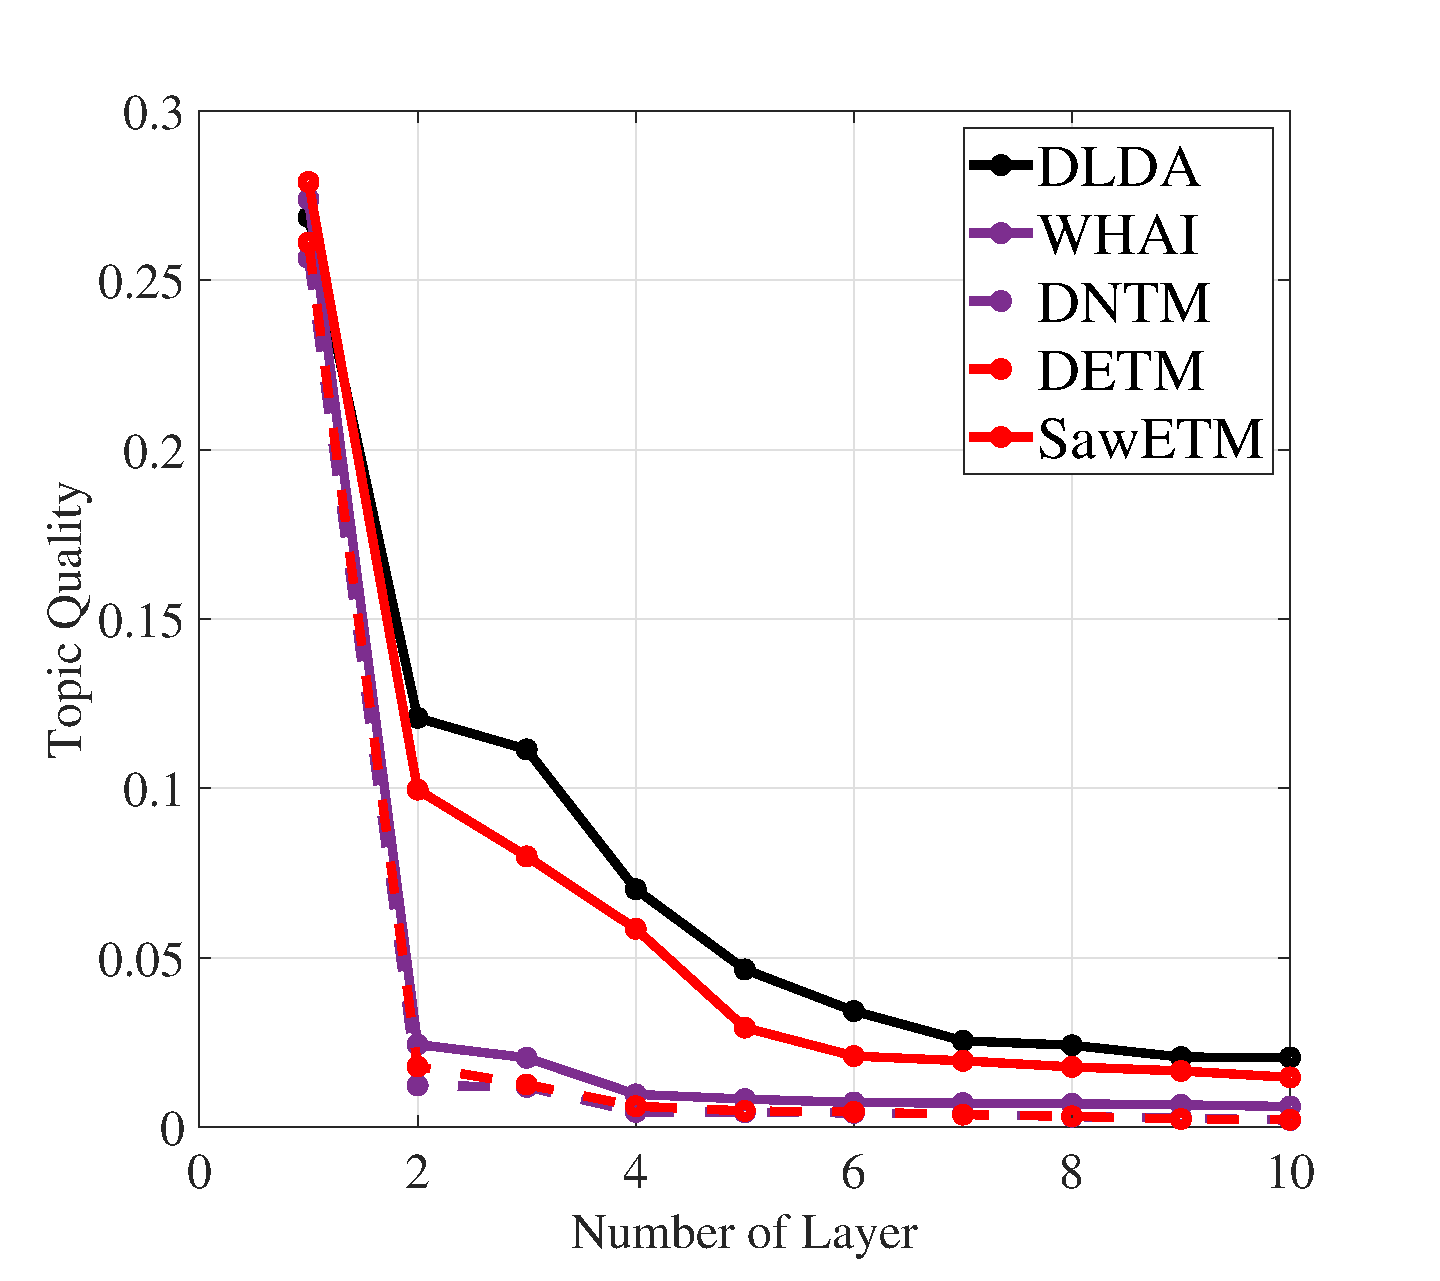
\includegraphics[width=0.31\linewidth]{quality_result/rcv1_quality.eps}
% } \hspace{-5mm}
% \quad 
% \subfigure[PG19]{
% 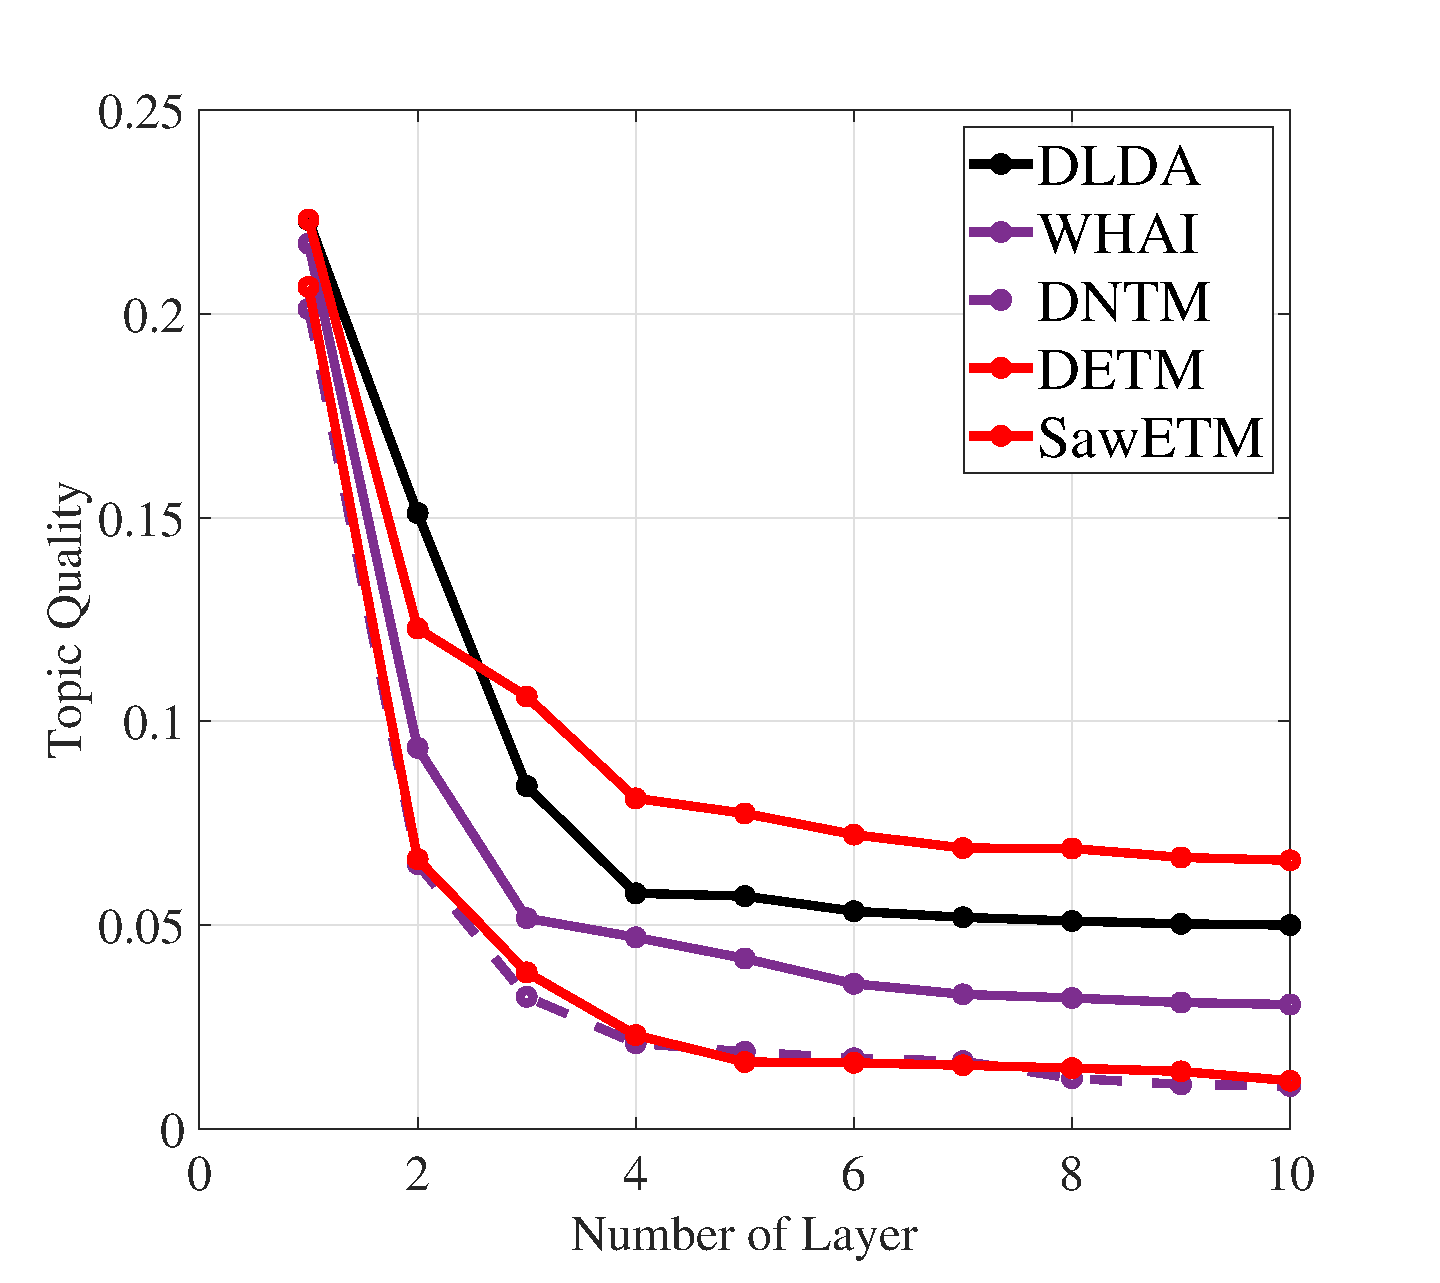
\includegraphics[width=0.31\linewidth]{quality_result/PG19_quality.eps}
% }
% \vspace{-3mm}
% \caption{(a)-(c) : Relative per-heldout-word perplexity (the lower the better), with the varied number of layers fixed proportion ($80\%$) of training words of each document. (d)-(f) : Topic quality as measured by normalized product of topic coherence and topic diversity (the higher the better) with the varied number of layers.}
% % and fixed the number of layers (5 layers for 20NG, and 8 layers for RCV1V2 and PG19)}
% \label{figure:PPl}
% \vspace{-3mm}
% \end{figure*}
\section{Experiments} 
We conducted extensive experiments to verify the effectiveness of Gaussian SawETM, TopicNet, and our novel TopicNet-TopNet integration. Our comprehensive evaluation includes both traditional topic modeling metrics and innovative cross-modal generation assessments. Our code is available at \url{https://github.com/BoChenGroup/TopicNet-TopNet}.  
% \vspace{-1mm}
% \subsection{Experimental Settings}
% \paragraph{Datasets. }Our experiments are conducted on five widely-used benchmark text datasets, varying in different sizes, including \textbf{R8} extracted from the Reuters-21578 dataset, 20 News Groups(\textbf{20NG}), Reuters Corpus Volume 2 (\textbf{RCV2}) and \textbf{Wiki} consists of 3 million documents randomly downloaded from Wikipedia using the script provided by Hoffman et al. \cite{hoffman2010online}.  In particular, R8 and 20NG are small dataset with document labels;RCV2 and Wiki are big dataset. The detailed description of all the datasets as attached in the supplement.
% \paragraph{Baseline methods and their settings: } We compare Gaussian SawETM with the state-of-the-art topic models: \textbf{1. LDA Group}, single layer topic models, including: Latent Dirichlet Allocation(\textbf{LDA}) \cite{blei2003latent}, which is a basic probability topic model and closely related to a single-hiddenlayer version of DLDA;  LDA with Products of Experts (\textbf{AVITM})  \cite{srivastava2017autoencoding}, which replaces the mixture model in LDA with a product of experts and uses the AVI for training; Embedding topic model(\textbf{ETM})  \cite{dieng2020topic}, which is a topic model that incorporates word embeddings and is
% learned by AVI. \textbf{2. DLDA group}, including: Deep latent allocation inferred by Gibbs sampling (\textbf{DLDA-Gibbs})  \cite{zhou2015poisson}  and  by TLASGR-MCMC \textbf{DLDA-TLASGR} \cite{cong2017deep}; Deep neural topic model(\textbf{WHAI})  \cite{zhang2018whai}, which use a Weibull upward-downward variational encoder to infer multilayer latent representation under DLDA and
% learned by AVI.Deep embedding topic model (\textbf{SawETM}) \cite{duan2021sawtooth}, which is a DLDA that incorporates word embedding and is learned by AVI. As shown in  \citep{cong2017deep}, DLDA-Gibbs and DLDA-TLASGR are state-of-the-art topic modeling methods that clearly outperform a large number of previously propose ones, such as replicated softmax  \cite{hinton2009replicated} and the nested Hierarchical Dirichlet procee  \cite{paisley2014nested}.  The hyperparameters settings we used for DLDA group are similar to the one used in  \cite{zhang2018whai, duan2021sawtooth}, while LDA group are their official code with the best reported settings.
%  LDA  \cite{blei2003latent}& 1 & 1 &60.9$\pm$0.7 &43.2$\pm$0.7 & $53.8\pm$0.6 & 36.9$\pm$0.6 \\
%     PFA  \cite{zhou2012beta} &61.2$\pm$0.3 &73.4$\pm$0.4 &61.9$\pm$0.5 &44.1$\pm$0.4 & $54.7\pm$0.5 & 37.6$\pm$0.4\\
%     \midrule
%     GAE  \cite{kipf2016variational} &65.8$\pm$0.4 & 77.0$\pm$0.4 &68.9$\pm$0.4 &52.8$\pm$0.3 &67.2$\pm$0.4 &44.5$\pm$0.4 \\
%     NVITM  \cite{xun2016topic} &66.3$\pm$0.2 & 77.2$\pm$0.2 &69.0$\pm$0.3 &53.0$\pm$0.3 &67.4$\pm$0.3 &44.6$\pm$0.3 \\
%     ETM  \cite{dieng2020topic} &66.5$\pm$0.2 & 77.3$\pm$0.2 &69.2$\pm$0.4 &53.3$\pm$0.3 &67.5$\pm$0.3 &44.8$\pm$0.3 \\
%     \midrule
%     PGBN-layer1  \cite{zhou2016augmentable} &70.7$\pm$0.6 &82.8$\pm$0.5 &71.5$\pm$0.7 &55.6$\pm$0.6 &70.4$\pm$0.7 &45.9$\pm$0.6\\
%     PGBN-layer5 &73.2$\pm$0.5 &84.6$\pm$0.4  &72.0$\pm$0.6 &56.1$\pm$0.6 &72.4$\pm$0.7 &46.8$\pm$0.5 \\
%     WHAI-layer1 &73.6$\pm$0.5 &85.0$\pm$0.5  &72.3$\pm$0.5 &56.5$\pm$0.4 &73.3$\pm$0.5 &47.5$\pm$0.4\\
%     WHAI-layer5  \cite{zhang2018whai} &78.7$\pm$2.5 &88.2$\pm$0.7 &72.5$\pm$1.8 &56.8$\pm$0.9 &73.8$\pm$1.4 &47.8$\pm$1.1 \\
%     SawETM-layer1  \cite{duan2021sawtooth}  &77.5$\pm$0.4 &87.7$\pm$0.4 &74.2$\pm$0.4 &58.3$\pm$0.3 &76.4$\pm$0.4 &50.3$\pm$0.4 \\
%     SawETM-layer5  &79.1$\pm$0.2 &88.1$\pm$0.3 &74.6$\pm$0.3 &58.7$\pm$0.2 &77.3$\pm$0.3 &51.0$\pm$0.5 \\
%     \midrule
%     Gaussian SawETM-layer1  &80.5$\pm$0.5 &87.9$\pm$0.4 &74.5$\pm$0.4 &58.6$\pm$0.3 &77.5$\pm$0.5 &51.1$\pm$0.4 \\
%     Gaussian SawETM-layer5   &82.3$\pm$0.4 &89.0$\pm$0.4 &75.0$\pm$0.3 &59.3$\pm$0.2 &78.0$\pm$0.4 &52.0$\pm$0.3 \\
%   TopicNet-layer1  &\textbf{83.3}$\pm$0.2 &\textbf{89.5}$\pm$0.2 &\textbf{75.3}$\pm$0.3 &\textbf{59.5}$\pm$0.3 &\textbf{78.2}$\pm$0.3 &\textbf{52.3}$\pm$0.3 \\
%   TopicNet-layer5  &\textbf{83.3}$\pm$0.2 &\textbf{89.5}$\pm$0.2 &\textbf{75.3}$\pm$0.3 &\textbf{59.5}$\pm$0.3 &\textbf{78.2}$\pm$0.3 &\textbf{52.3}$\pm$0.3 \\

%  \midrule
%     WHAI & 1& & & \\
%     WHAI &5 & & & \\
%     WHAI & 15& & & \\
%     \midrule
%     SawETM & 1& & & \\
%     SawETM &5 & & & \\
%     SawETM &15 & & & \\
%     \midrule
%     Gaussian SawETM &1 & & & \\
%     Gaussian SawETM &5 & & & \\
%     Gaussian SawETM &15 & & & \\

% \subsection{Experiments of Guassian SawETM}

%  Note that, for fair caparison with other topic models, we use the same network structure with  \cite{duan2021sawtooth}. And then 
%  and don't compare TopicNet in this section because the network structure is defied by knowledge graph.
\paragraph{Baseline methods and their settings:} We compare Gaussian SawETM with the state-of-the-art topic models: {1. LDA Group}, including: latent Dirichlet allocation(\textbf{LDA}) \cite{blei2003latent}, which is a basic probabilistic topic model; LDA with Products of Experts (\textbf{AVITM})  \cite{srivastava2017autoencoding}, which replaces the mixture model in LDA with a product of experts and uses the AVI for training; Embedding Topic Model (\textbf{ETM}) \cite{dieng2020topic}, a generative model that incorporates word embeddings into traditional topic model. 
{2. DLDA Group}, including: Deep LDA inferred by Gibbs sampling (\textbf{DLDA-Gibbs}) \cite{zhou2015poisson}  and  by TLASGR-MCMC (\textbf{DLDA-TLASGR}) \cite{cong2017deep}. {3. Deep Neural Topic Model (DNTM) Group}, including Weibull Hybrid Autoencoding Inference model (\textbf{WHAI}) \citep{zhang2018whai}, which employs a deep variational encoder to infer hierarchical document representations, and Sawtooth Factorial Embedded Topic Model (\textbf{SawETM}) \citep{duan2021sawtooth}, where topics are modeled as learnable deterministic vectors. For all baselines, we use their official default parameters with best reported settings. 
% As shown in  \citep{cong2017deep}, DLDA-Gibbs and DLDA-TLASGR are state-of-the-art topic modeling methods that clearly outperform a large number of previously propose ones, such as replicated softmax  \cite{hinton2009replicated} and the nested Hierarchical Dirichlet procee  \cite{paisley2014nested}.

 \paragraph{Datasets} Our experiments are conducted on four widely-used benchmark datasets, including 20Newsgroups ({20NG}), Reuters Corpus Volume I ({RCV1}), Wikipedia ({Wiki}), and a subset of the Reuters-21578 dataset ({R8}), varying in scale and document length. 20NG, with a vocabulary of 2$,$000 words, has 20 classes and was split into 11$,$314 training and 7$,$532 test documents. RCV1 consists of 804$,$414 documents with a vocabulary size of 8$,$000. Wiki, with a vocabulary size of 10$,$000, consists of 3 million documents randomly downloaded from Wikipedia using the script provided by \citet{hoffman2010online}. R8, with a vocabulary size of 10$,$000, has 8 classes and was split into 5$,$485 training and 2$,$189 test documents. The summary statistics of these datasets and other implementation details (such as dataset preprocessing and length statistics) are described in the Appendix. 
% size of 2,000 consists of 18,845 documents with 20 categories. Following \cite{yao2019graph}, we build the vocabulary with size 36,534 after removing stopwords and low-frequency words appearing less than 5 times. The average document length is 221. \textbf{2. RCV1}, Reuters Corpus Volume I, consists of 804,414 documents \cite{lewis2004rcv1}. The vocabulary contains 8$,$000 tokens and there are words in one document on average 140. \textbf{3. PG-19} is a using text from books extracted from Project Gutenberg \cite{raecompressive2019}. The dataset contains 28,752 books or 11GB of text. with a vocabulary size of 20,000. We split each book by 1024 tokens, resulting in 613,386 documents. Note that the first two datasets are used for document clusters experiment due to there are ground-truth labels and the last three datasets are used for other experiments.
%  including a subset of the Reuters-21578 dataset(\textbf{R8}), 20 News Groups (\textbf{20NG}) consists of 18,845 documents with a vocabulary size of 2,000, Reuters Corpus Volume 2 (\textbf{RCV2}) and \textbf{Wiki}, which \cite{hoffman2010online}.
%  %In particular, 20NG is small dataset, while RCV2 and Wiki are big datasets.
\begin{table}
    \centering
    \caption{\small Comparison of per-heldout-word perplexity on three different datasets.}
    \label{tab:perplexity}
    \scalebox{0.75}{
    \begin{tabular}{c|c|c|c|c|c|c|c|c|c}
    \toprule
    \textbf{Method} &\textbf{Depth}&\textbf{20NG}&\textbf{RCV1} & \textbf{Wiki} & \textbf{Method} &\textbf{Depth}&\textbf{20NG}&\textbf{RCV1} & \textbf{Wiki}   \\
    \midrule
    %K-means  &68.3 &73.4 &25.9 &55.1 &61.2 &74.7 \\
    %NCut  \cite{shi2000normalized} &69.6 &79.2 &65.9 &80.3 &71.2 &76.5 \\ \hline
    %SVD  &64.3 &74.5 & & & & \\
    LDA \cite{blei2003latent}& 1 & 735 & 942 &1553  &DNTM-WHAI \cite{zhang2018whai}&1& 762& 952&1657 \\
    AVITM \cite{xun2016topic}&1 & 784 & 968& 1703& DNTM-WHAI \cite{zhang2018whai}&5 & 726& 906&1595 \\
    ETM \cite{dieng2020topic}&1 & 742& 951 & 1581& DNTM-WHAI \cite{zhang2018whai}& 15 & 724 &902 &1592 \\
    \midrule
    DLDA-Gibbs \cite{zhou2015poisson}& 1& 702 & - & - &DNTM-SawETM \cite{duan2021sawtooth}& 1& 718& 908&1536 \\
    DLDA-Gibbs \cite{zhou2015poisson}&5 & 678 & - & - &DNTM-SawETM \cite{duan2021sawtooth}& 5&688&873& 1503\\
    DLDA-Gibbs \cite{zhou2015poisson}& 15 & 670 & - & - &DNTM-SawETM \cite{duan2021sawtooth}& 15& 684& 864&1492 \\
    \midrule
    DLDA-TLASGR \cite{cong2017deep} &1&714&912 &1455 &DNTM-GaussSawETM &1 & 714& 904& 1529 \\
    DLDA-TLASGR \cite{cong2017deep} &5&684&877& 1432&DNTM-GaussSawETM &5 & 685&866 & 1477 \\
    DLDA-TLASGR \cite{cong2017deep} &15&673& 842& 1421&DNTM-GaussSawETM &15 & 678& 857&1452 \\
    \bottomrule
    \end{tabular}}
\end{table}
\subsection{Unsupervised learning for document representation} 
\paragraph{Per-heldout-word perplexity:} To measure predictive quality of the proposed model, we calculate the per-heldout-word perplexity (PPL)  \cite{cong2017deep}, on three regular document datasets, $e.g.$, 20NG, RCV1, and Wiki. For deep topic models in the DLDA and DNTM groups, we report the PPL with 3 different stochastic layers $T \in \{1, 5, 15\}$. Specifically, for a 15-layer model, the topic size from bottom to top is set as $\mathbf{K} = [256, 224, 192, 160, 128, 112, 96, 80, 64, 56, 48, 40, 32, 16, 8]$, and the detailed description can be found in the Appendix. For each corpus, we randomly select 80\% of the word tokens from each document to form a training matrix ${\rm{X}}$, holding out the remaining 20\% to form a testing matrix ${\rm{Y}}$. We use ${\rm{X}}$ to train the model and calculate the per-held-word perplexity as
 $$\textstyle \exp \left\{ { - {1 \over {{y_{..}}}}\sum\limits_{v = 1}^V {\sum\limits_{n = 1}^N {{y_{vn}}\ln {{\sum\nolimits_{s = 1}^S {\sum\nolimits_{k = 1}^{{K^1}} {\phi _{vk}^{\left( 1 \right)s}\theta _{kn}^{\left( 1 \right)s}} } } \over {\sum\nolimits_{s = 1}^S {\sum\nolimits_{v = 1}^V {\sum\nolimits_{k = 1}^{{K^1}} {\phi _{vk}^{\left( 1 \right)s}\theta _{kn}^{\left( 1 \right)s}} } } }}} } } \right\},$$ where $S$ is the total number of collected samples and ${y_{ \cdot  \cdot }} = \sum\nolimits_{v = 1}^V {\sum\nolimits_{n = 1}^N {{y_{vn}}} }$.
 As shown in Tab.~\ref{tab:perplexity}, overall, DLDA-Gibbs perform best in terms of PPL, which is not surprising as they can sample from the true posteriors given a sufficiently large number of Gibbs sampling iterations. DLDA-TLASGR is a mini-batch based algorithm that is much more scalable in training than DLDA-Gibbs, at the expense of slightly degraded performance in out-of-sample prediction. Apart from these deep probabilistic topic models, Gaussian SawETM outperforms other neural topic models in all datasets. In particular, compared with Gaussian based single layer neural topic model, WHAI performs better, which can be attributed to two aspects, the first is the effectiveness of Weibull distribution in modeling sparse and non-negative document latent representations, and the second is aggregating the information in both the higher (prior) layer and that upward propagated to the current layer via inference network. Benefiting from the embedding decoder and the Sawtooth Connection that builds the dependency of hierarchical topics, SawETM performs better than WHAI, especially at deeper layers. However, modeling topics with point vectors, SawETM cannot capture the uncertainties of topics. Gaussian SawETM represents the topics with Gaussian-distributed embeddings to capture the uncertainties, and achieves promising improvements over SawETM, especially for modeling complex and big corpora such as Wiki. Note that although the methods in DLDA group get better performance, they require iteratively sampling to infer latent document representations in the test stage, which limits their application \cite{zhang2018whai}. By contrast, Gaussian SawETM can infer latent representations via direct projection, which makes it both scalable to large corpora and fast in out-of-sample prediction.
 %Gaussian SawETM  perform better compared with , which p Gibbs sampling based models perform the best in terms of PPL,  which is not surprising as they can sample from the true posteriors given a sufficiently large number of Gibbs sampling iterations. Compared with methods in LDA and DLDA groups, GaussianSawETM achieves comparable performance, and outperforms them on RCV1 datasets. As shown in Table.~\ref{tab:perplexity},  given the same generative network structure, DLDA-Gibbs performs the best in terms of predicting heldout word tokens, which is not surprising as this batch algorithm can sample from the true posteriors given a sufficiently large number of Gibbs sampling iterations. DLDA-TLASGR is a mini-batch algorithm that is much more salable in training than DLDA-Gibbs, at the expense of slightly degraded performance in out-of-sample prediction. 
 %Overall, Gaussian SawETM get comparable results with the models in DLDA group and better results with the other neural topic model. 
%  capture the unseatian of both words and topics, and result in best results in naural topic model. compared with the methods in the LDA group that are limited to single layer shallow models, the hierarchical topic model in the DLDA group aggregate the information in both document and hierarchical prior via the gamma belief network, exhibiting better performance. With Compared with the methods in the DLDA group that need to perform Gibbs sampling at the testing stage, the methods in the DATM group are considerably faster in processing a testing document, due to the use of an inference network.
%  However, the methods in the DLDA group is , which in 
%  However, those graph autoencoders focus obsessively on the generation of the edges but ignore the node generation, leading to worse performance relative to the models in group three, indicating the importance of node generation in clustering tasks.
% Among these graph-based models in group three, the proposed GPFA outperforms traditional RTM, attributed to the more accurate posterior estimations.
% With a controllable weight that balances the node and edge generations, WGAEs and WGCAEs further improve the clustering performance, where WGCAEs, benefiting from the effectiveness of GCN in graph representation, achieve higher scores than WGAEs under the same network structure settings.
% Moreover, the performance improvement of PGBN over LDA, GPGBN over GPFA, and multilayer WGAE/WGCAE over single-layer WGAE/WGCAE demonstrate that the richer semantics provided by a deeper probabilistic model can boost the clustering performance.
%  In the first group, ETM gets the best performance compared with LDA and AVITM, which can be attributed to the embedding decoder. LDA has the better performance compared with AVITM, which is not surprising as this batch algorithm can sample from the true posteriors given enough Gibbs sampling iterations. But these models are limited to single layer shallow models, which can't benefit from the deep structure and results in the gap with the second group of models. The performance of DLDA-Gibbs and DLDA-TLASGR can be improved by increasing the number of layers effectively, but WHAI can not improve performance when layer size greater than three. Besides, although the DNTM and DETM having the same encoder with SawETM, they can't have obvious performance improvement when the number of layers greater than three, too. We attribute this to the reason that all layers of the natural topic models are trained together, which makes it difficult to learn meaningful prior.  Benefiting from the sawtooth connection(SC) between different layers, the topic information at lower layers can flow to the upper network, which can help the higher layer learn the meaningful topic, and results in better prior learned by SawETM. We can see that SawETM have better performance with a bigger layer size, and get comparable performance with DLDA
% Note that the experimental results for LDA and PGBN-Gibbs on Rcv1/PG19 datasets are not exhibited, due to the fact that Gibbs Sampling requires too much computer memory for a big dataset. 
% In the first group, ETM gets the best performance compared with LDA and AVITM, which can be attributed to the embedding decoder. LDA has the better performance compared with AVITM, which is not surprising as this batch algorithm can sample from the true posteriors given enough Gibbs sampling iterations. But these models are limited to single layer shallow models, which can't benefit from the deep structure and results in the gap with the second group of models. 
% The performance of DLDA-Gibbs and DLDA-TLASGR can be improved by increasing the number of layers effectively, but WHAI can not improve performance when layer size greater than three. Besides, although the DNTM and DETM having the same encoder with SawETM, they can't have obvious performance improvement when the number of layers greater than three, too. We attribute this to the reason that all layers of the natural topic models are trained together, which makes it difficult to learn meaningful prior. And similar to deep VAE, this phenomenon is called mode collapse  \cite{maaloe2019biva}. Benefiting from the sawtooth connection(SC) between different layers, the topic information at lower layers can flow to the upper network, which can help the higher layer learn the meaningful topic, and results in better prior learned by SawETM. We can see that SawETM have better performance with a bigger layer size, and get comparable performance with DLDA.
% \subsection{Experiments of TopicNet}
% \paragraph{Datasets $\&$ Model Settings:} We consider using 
\begin{table}
    \centering
    \caption{\small Comparison of document classification and clustering performance.}
    \label{tab:graph_cluster}
    \scalebox{0.80}{
    \begin{tabular}{c|c|cc|cc|cc}
    \toprule
    \textbf{Methods}&\textbf{Depth} &\multicolumn{2}{c|}{\textbf{Classification}}
    &\multicolumn{4}{c}{\textbf{Clustering}} \\
    & &\textbf{20NG}&\textbf{R8}    &\multicolumn{2}{c}{\textbf{20NG}} &\multicolumn{2}{c}{\textbf{R8}} \\
    & & & & ACC &NMI &ACC &NMI \\
    \midrule
    %K-means  &68.3 &73.4 &25.9 &55.1 &61.2 &74.7 \\
    %NCut  \cite{shi2000normalized} &69.6 &79.2 &65.9 &80.3 &71.2 &76.5 \\ \hline
    %SVD  &64.3 &74.5 & & & & \\
    LDA \cite{blei2003latent}& 1 &72.6$\pm$0.3 &88.4$\pm$0.5 &46.5$\pm$0.2 &45.1$\pm$0.4 & $51.4\pm$0.4 & 40.5$\pm$0.3 \\
    NVITM \cite{xun2016topic}& 1 &71.5$\pm$0.4 & 87.3$\pm$0.2 &48.3$\pm$0.5 &46.4$\pm$0.3 &52.5$\pm$0.2 &41.2$\pm$0.4 \\
    ETM \cite{dieng2020topic}& 1 &71.9$\pm$0.2& 87.9$\pm$0.4 &49.8$\pm$0.6 &48.4$\pm$0.5 &55.3$\pm$0.4 &42.3$\pm$0.2 \\
    \midrule
    PGBN \cite{zhou2016augmentable}&1&74.2$\pm$0.5 &90.8$\pm$0.5 &46.6$\pm$0.5 &45.4$\pm$0.6 &51.7$\pm$0.4 &40.7$\pm$0.4\\ 
    PGBN \cite{zhou2016augmentable}&4&76.0$\pm$0.3 &91.6$\pm$0.4  &48.2$\pm$0.2 &46.5$\pm$0.5 &54.4$\pm$0.4 &41.2$\pm$0.3 \\ 
    \midrule
    WHAI \cite{zhang2018whai}& 1 &72.8$\pm$0.3 &85.3$\pm$0.2  &49.4$\pm$0.5 &46.5$\pm$0.4 &57.9$\pm$0.5 &42.3$\pm$0.4\\
    WHAI \cite{zhang2018whai}& 4 &73.7$\pm$0.5 &88.4$\pm$0.3 &
    49.5$\pm$0.4 &47.0$\pm$0.3 &60.4$\pm$0.4 &44.1$\pm$0.2 \\ 
    \midrule
    SawETM \cite{duan2021sawtooth}& 1 &70.5$\pm$0.3 &88.6$\pm$0.2 &50.2$\pm$0.2 &48.7$\pm$0.3 &61.2$\pm$0.4 &43.4$\pm$0.4 \\
    SawETM \cite{duan2021sawtooth}& 4 &71.1$\pm$0.2 &90.5$\pm$0.3 &51.2$\pm$0.3 &50.7$\pm$0.2 &63.8$\pm$0.3 &45.9$\pm$0.5 \\
    \midrule
    Gaussian SawETM& 1  &72.8$\pm$0.3 &89.8$\pm$0.4 
    &51.3$\pm$0.4 &50.6$\pm$0.2 &61.5$\pm$0.3 &44.1$\pm$0.2 \\
    Gaussian SawETM& 4   &75.2$\pm$0.4 &91.0$\pm$0.3
    &53.0$\pm$0.3 &51.3$\pm$0.2 &65.2$\pm$0.4 &47.0$\pm$0.3 \\ 
    \midrule
   TopicNet& 1  &71.6$\pm$0.2&88.6$\pm$0.3 & 49.5$\pm$0.3 &46.3$\pm$0.4 & 61.0$\pm$0.2& 43.2$\pm$0.3\\
   TopicNet& 4  &74.3$\pm$0.5&89.5$\pm$0.4 & 50.8$\pm$ 0.3& 47.8$\pm$0.4&64.2$\pm$0.3&46.5$\pm$0.2 \\
  \bottomrule
  \end{tabular}}
\end{table}
\paragraph{Document Classification $\&$ Clustering}
Document-topic distributions can be viewed as unsupervised document representations, to evaluate their quality, we perform document classification and clustering tasks. In detail, we first use the trained topic models to extract the latent representations of the testing documents and then use logistic regression to predict the label and use k-means to predict the clusters. we measure the classification performance by classification accuracy, and clustering performance by accuracy (ACC) and normalized mutual information (NMI), both of which are the higher the better. we test the model performance on 20NG and R8, where the document labels are considered. Different from the perplexity experiments, a larger vocabulary of 20$,$000 words is used for 20News to achieve better performance. The network structure is defined by TopicTree, which is introduced in Section~\ref{sec:topictree}, with the details  deferred to the Appendix. The comparison results are summarized in Tab.~\ref{tab:graph_cluster}. Benefiting from the use of Gaussian distributions on topics, Gaussian SawETM outperforms the other neural topic models on not only  document classification  but also clustering, demonstrating its effectiveness of extracting document latent representations. Note that Gaussian SawETM acquires promising improvements compared to SawETM in the 20NG dataset, showing the potential for modeling more complex data. With the predefined knowledge prior, TopicNet does not perform better, possibly because the introduced prior information does not well align with the end task. We leave the refinement of prior information for specific tasks to future study.
%and we will explore how to build a task-related prior to improve the TopicNet's performance on special tasks. 

% For Table 2 of the original paper, we choose a vocabulary of 20,000 terms, which has 4693 terms that overlap with the vocabulary of the WordNet. Using these 4693 shared terms, we extract a [4693,496,89,11,2] subgraph as the prior WordNet. With not only a larger vocabulary size, but also a wider first topic layer (496 topics instead of 314 topics), it is hence not surprising that a better performance can be achieved for downstream tasks.
% Choosing a vocabulary of 2000 terms (words) for the 20 newsgroups, we compare the 2000 terms to these in the WordNet, which consists of over 70,000 terms, and find 736 terms that are shared between the 20newsgroups and WordNet. Extracting a four-layer subgraph from the WordNet that are rooted at these 736 terms, we obtain a prior WordNet with [736,314,152,52,11] nodes from the bottom to top layers.  
%\mz{do you mean logistic regression/a linear classifier?
% It can be observed that with word embedding and sawtooth connection, SawETM extracts more separable document latent representations  and outperforms the other comparison methods.
% and report the purity and Normalized Mutual Information (NMI) on 20NG, and R8, where the document labels are considered.  With the default training/testing splits of the datasets, we train a model on
% the training documents and infer the topic distributions z on the testing documents.
\subsection{Interpretable topic discovery}
Apart from excelling at document representation learning, another appealing characteristic of TopicNet is that it can discover interpretable hierarchical topics. In this section, we perform the topic discovery experiment with a $7$-layer TopicNet trained on 20NG. The network structure is constructed corresponding to the structure of TopicTree, which is set as $\text{[411, 316, 231, 130, 46, 11, 2]}$. 
% \paragraph{Document Classification $\&$ Clustering}
% We construct the semantic graph from WordNet in all experiments/datasets. 
\paragraph{Prior knowledge and corresponding learned topic:} 
We show six example topics %(out of 314 nodes from the bottom topic layer) 
and their corresponding children nodes in Tab.~\ref{tab:Concept_topic}, which illustrates how a particular concept is being represented in the 20 newsgroups. 
For example, the “military$\_$action” concept, which has “assault”, “defense”, 
and “war” as its children nodes, has become tightly connected to the Waco Siege heavily discussed in this dataset;
the “macromolecule” concept, which has “oil” as its single child node, has been represented by a topic related to vehicle, which is interesting as the 20newsgroups dataset has the following two newsgropus--- “rec.autos’ and “rec.motorcycles”---but not a newsgroup clearly related to biology and chemistry; and the “Atmosphere” concept, which has “Sky” as its single child node, has been represented by a topic related to NASA, reflecting the fact that “sci.space” is one of the 20 news~groups.
%(out of 736 nodes from the bottom word layer) in the Table.~\ref{tab:Concept_topic}


\paragraph{Topic quality:} Two metrics are considered here to evaluate the topic quality. The first metric is topic coherence, which is computed by taking the average Normalized Pointwise Mutual Information (NPMI) of the top 10 words of each topic \cite{aletras2013evaluating}. It provides a quantitative measure of the semantic coherence of a topic. The second metric is topic diversity \cite{dieng2020topic}, which suggests the percentage of unique words in the top 25 words of all topics. Diversity close to 1 means more sundry topics. Following \citet{dieng2020topic}, we define topic quality as the product of topic coherence and topic diversity. Note that topic quality is affected by the topic size, so it makes sense to compare different models on the same layer.  As shown in Fig.~\ref{fig:topic_quality}, Gaussian SawETM performs better compared to SawETM, which can be attributed to the Gaussian-distributed embeddings that capture the semantic uncertainties of topics. Incorporating the hierarchical prior knowledge, TopicNet further achieves a higher score than Gaussian SawETM. However, it gets a lower score compared to DLDA-Gibbs in the first two layers, as the layer goes deeper, TopicNet performs better. This is easy to understand since information from data reduces slightly in the shallow layers but severely in the deep layers. 

%And similar to deep VAE, this phenomenon is called mode collapse \cite{maaloe2019biva}. Benefiting from the sawtooth connection(SC) between different layers, the topic information at lower layers can flow to the upper network, which can help the higher layer learn the meaningful topic, and results in better prior learned by SawETM. We can see that SawETM have better performance with a bigger layer size, and get comparable performance with DLDA.
% visitation 
\begin{wrapfigure}{r}{0.5\textwidth}
\begin{center} \vspace{-10mm}
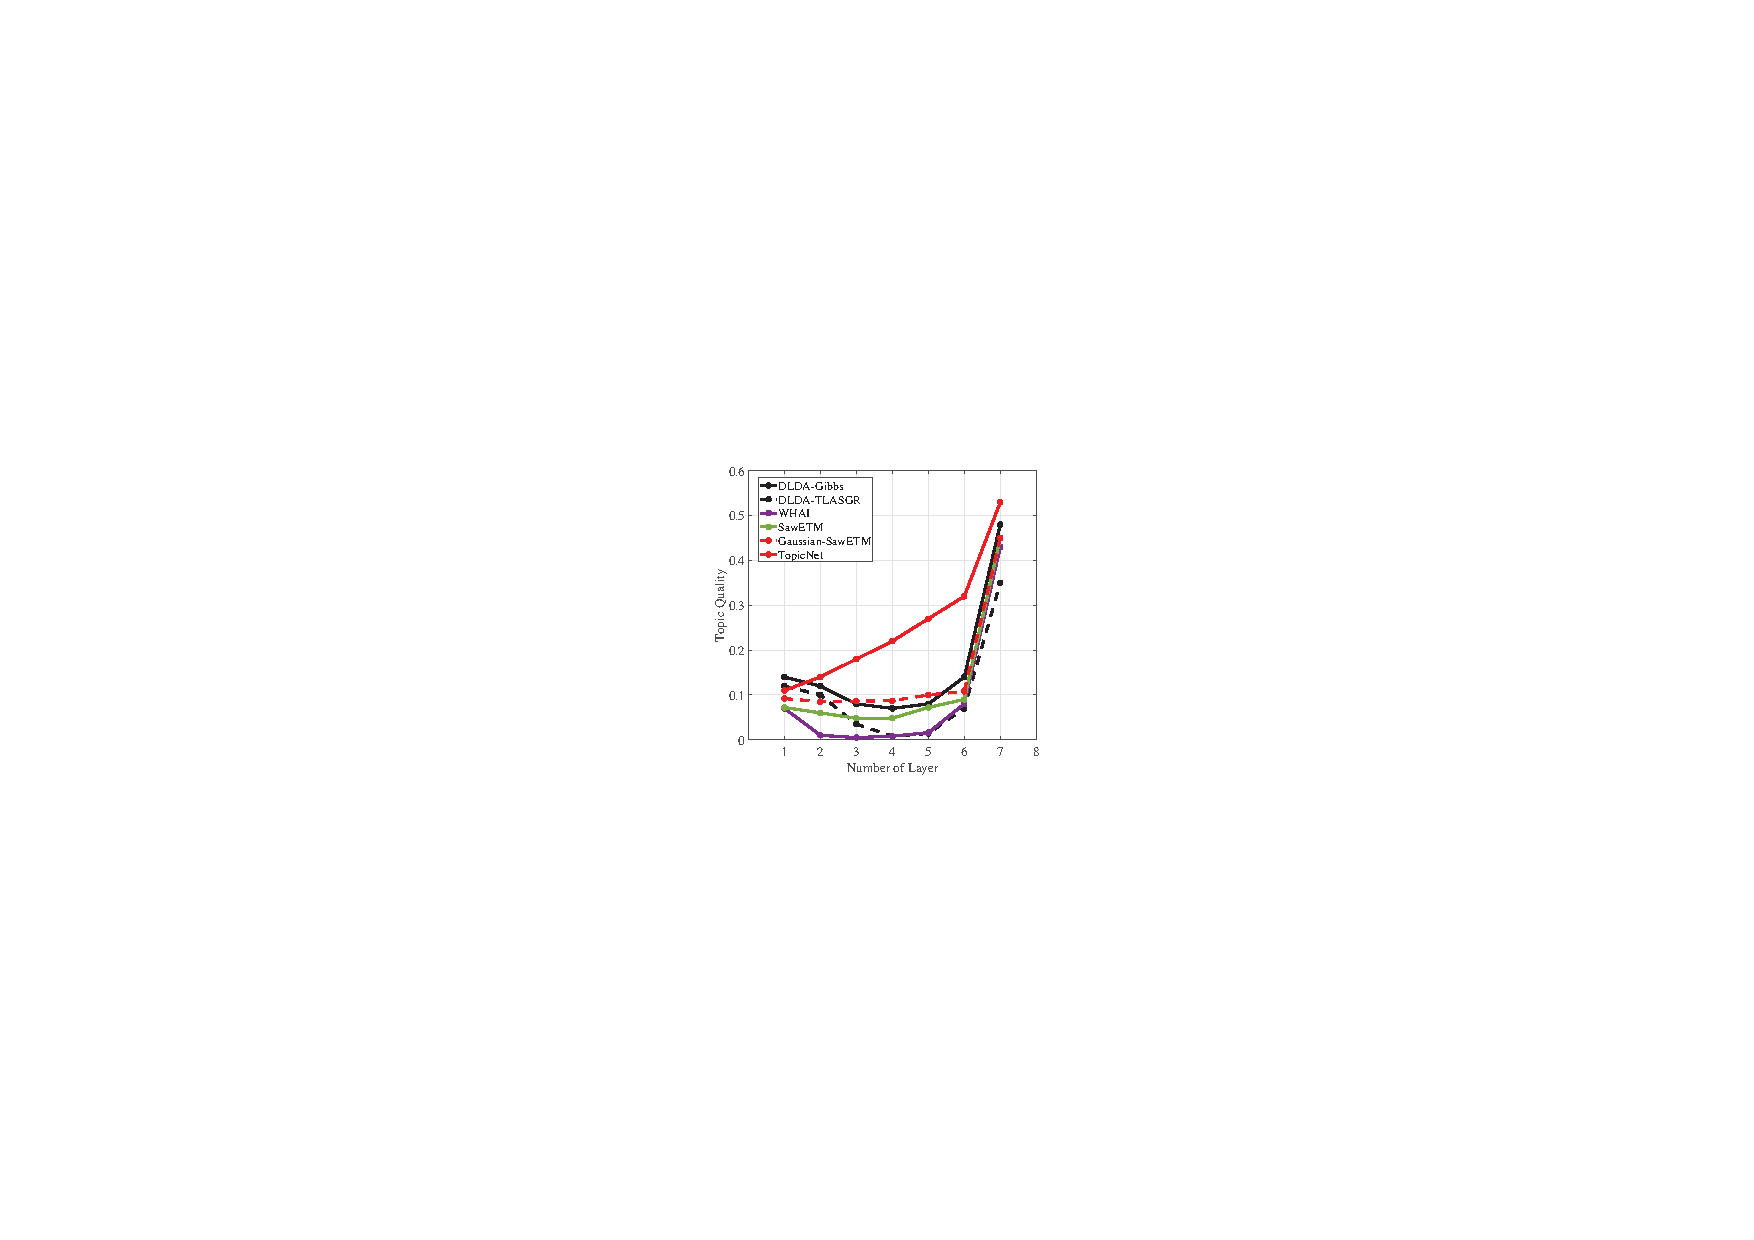
\includegraphics[width=0.45\textwidth]{quality_result/topic_quality_20ng.pdf} 
\end{center} \vspace{-4mm}
\caption{Topic quality as measured by normalized product of topic coherence and topic diversity (the higher the better) with the varied number of layers. Each layer's topic quality is influenced by its layer size, which is set as $\text{[411, 316, 231, 130, 46, 11, 2]}$ from the bottom layer to the top layer.} 
\label{fig:topic_quality} \vspace{-6mm}
\end{wrapfigure}
% \subsection{Qualitative Analysis}
\begin{table}
    \centering
    \caption{\small Semantic graph and corresponding learned topic on the bottom layer.}
    \label{tab:Concept_topic}
    \scalebox{0.80}{
    \begin{tabular}{c|c|c|c}
    \toprule
    \textbf{Topic}&\textbf{Concept} &\textbf{Children word nodes} &\textbf{Topic words} \\
    \midrule
    %K-means  &68.3 &73.4 &25.9 &55.1 &61.2 &74.7 \\
    %NCut  \cite{shi2000normalized} &69.6 &79.2 &65.9 &80.3 &71.2 &76.5 \\ \hline
    %SVD  &64.3 &74.5 & & & & \\
      11 & military$\_$action & assault defense war & \tabincell{c}{gun fbi guns koresh batf \\ waco assault children compound weapons} \\
    \midrule
      131 & coding$\_$system & \tabincell{c}{address shareware  \\ software unix windows} & \tabincell{c}{windows dos driver microsoft \\ drivers running applications unix using network}\\
    \midrule
     178 & macromolecule & oil & \tabincell{c}{car bike cars engine \\ oil  saturn ford riding miles road}\\
    \midrule
     186 & polity & government & \tabincell{c}{government law rights state \\ police right federal shall crime court laws}\\
    \midrule
     296 & atmosphere & sky & \tabincell{c}{space launch nasa gov \\ satellite earth mission shuttle hst orbit sky}\\
    \midrule
    298 & color & \tabincell{c}{black blue \\ brown color green red} & \tabincell{c}{color green blue red \\ black brown led subject showed lines}\\
    \bottomrule
    \end{tabular}}
\end{table}
\paragraph{Visualisation of embedding space:} First of all, we use a $\text{3}$-layer Gaussian SawETM with $\text{2}$-dim embedding trained on 20NG for the Gaussian-distribution embedding visualization. The top $\text{4}$ words from the $\mathtt{16 ^{th}}$ topic at $\mathtt{1 ^{th}}$ layer are visualized in Fig.~\ref{figure:word_embedding}. As we can see, the words under the same topic are closer in the embedding space, which demonstrates the learned embeddings are semantically similar. Apart from the semantics of words and topics, the shadow range describes the uncertainties and reflects the abstraction levels. Secondly, we visualize the means of Gaussian-distributed embeddings learned by TopicNet with T-SNE \cite{van2008visualizing}. As shown in Fig.~\ref{figure:topic_embedding}, in the shared embedding space, the words with similar semantics are close to each other, meanwhile they all locate near the topic that has similar semantics to them, which means the TopicNet effectively captures the prior semantic information and discovers more interpretable topics. 
\begin{figure*}[!ht]
\centering
\subfigure[Words Embedding]{
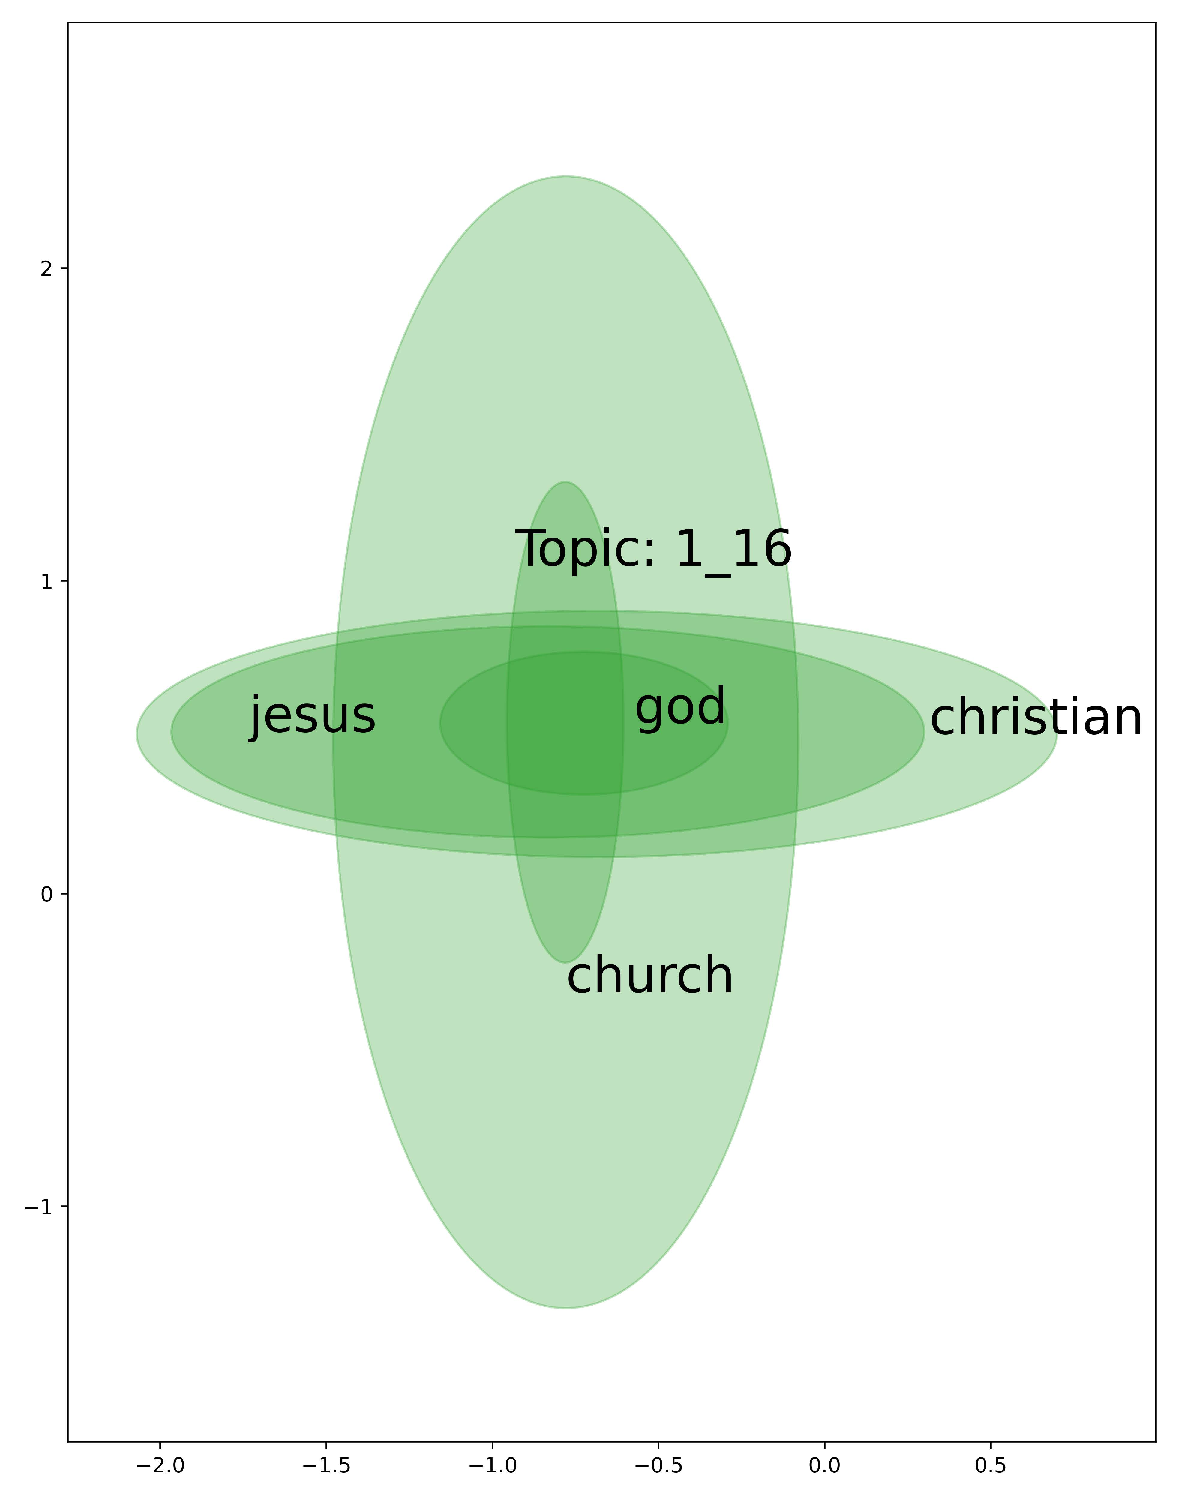
\includegraphics[width=0.28\linewidth]{TopicNet_vis/gaussian_embedding_vislization.pdf}
\label{figure:word_embedding}
}
\quad
\subfigure[Topic Embedding]{
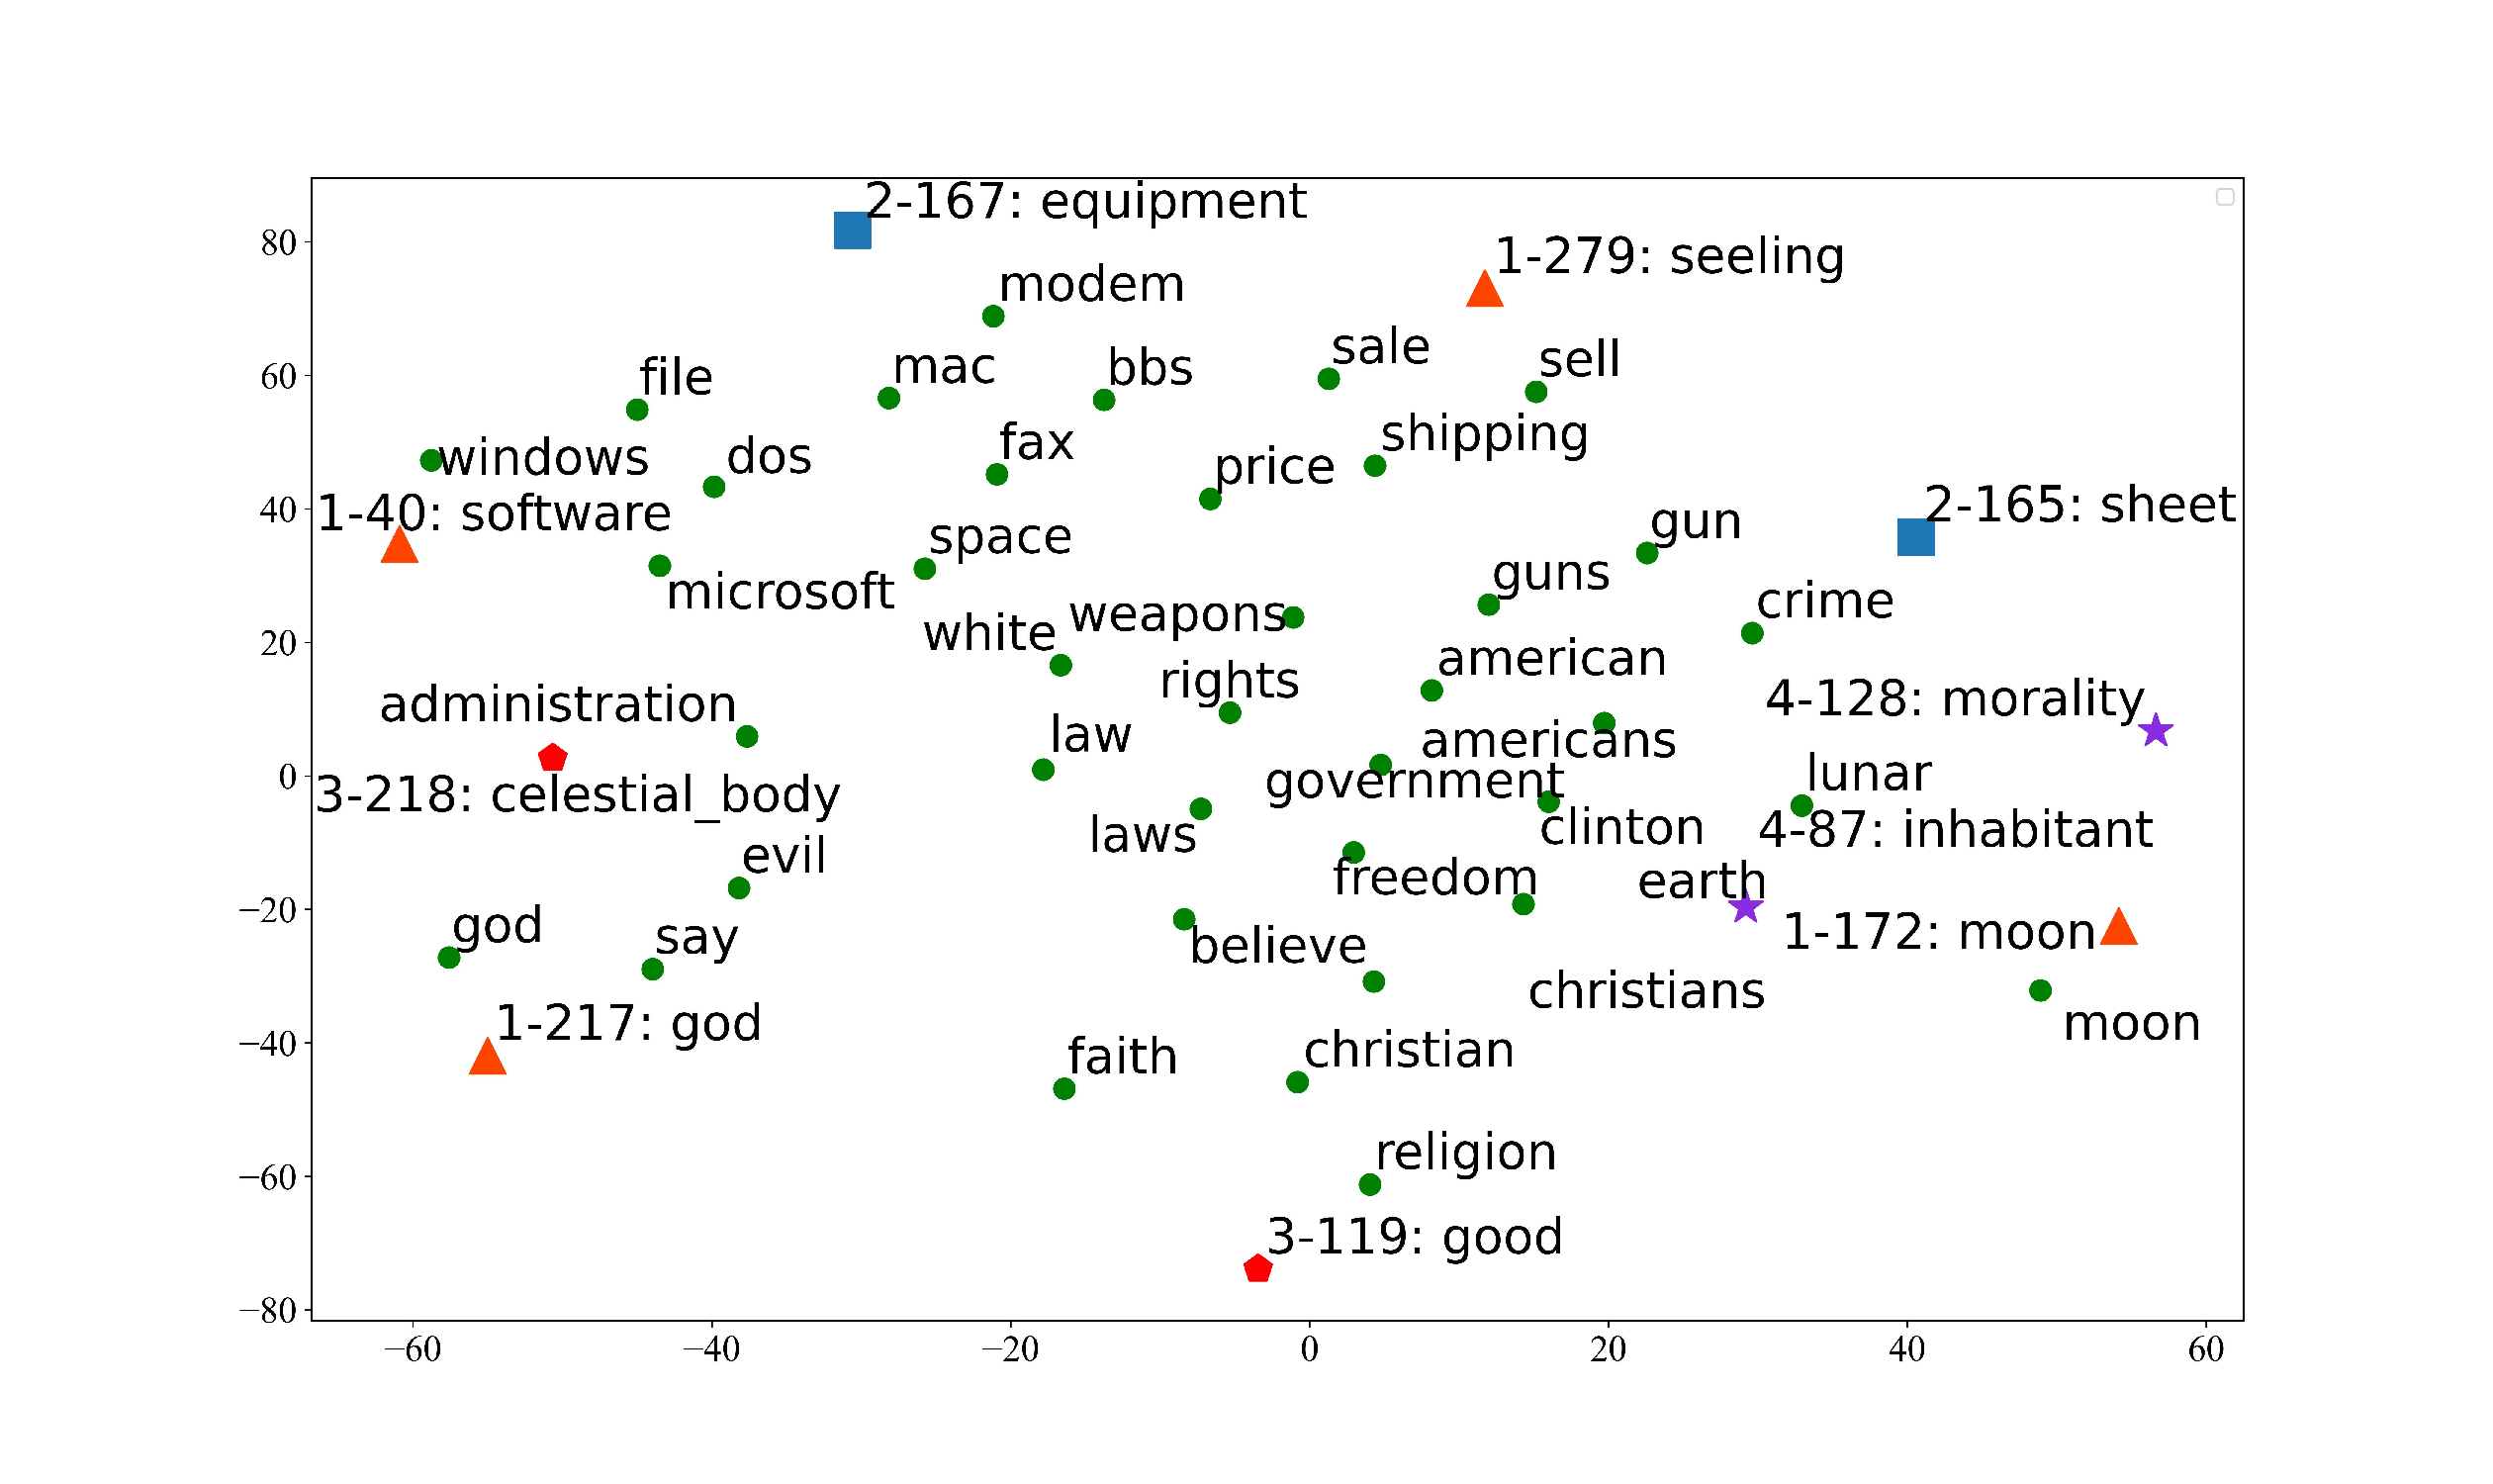
\includegraphics[width=0.60\linewidth]{TopicNet_vis/word_embedding_hier_wordnet.pdf}} 
\label{figure:topic_embedding} \vspace{-2mm}
\caption{(a) 2-dim Gaussian embedding in Gaussian SawETM, which we choose the top four words for the topic and (b) T-SNE visualisation of the mean of Gaussian distribution embedding in TopicNet. (The Topic: $\mathtt{t}$-$\mathtt{j: xx}$ denotes the $\mathtt{j ^{th}}$ topic at $\mathtt{t ^{th}}$ layer and $\mathtt{xx}$ represent the concept about the topic.)} 
\label{figure:embedding}
\end{figure*}
\begin{figure*}[!h]
\centering
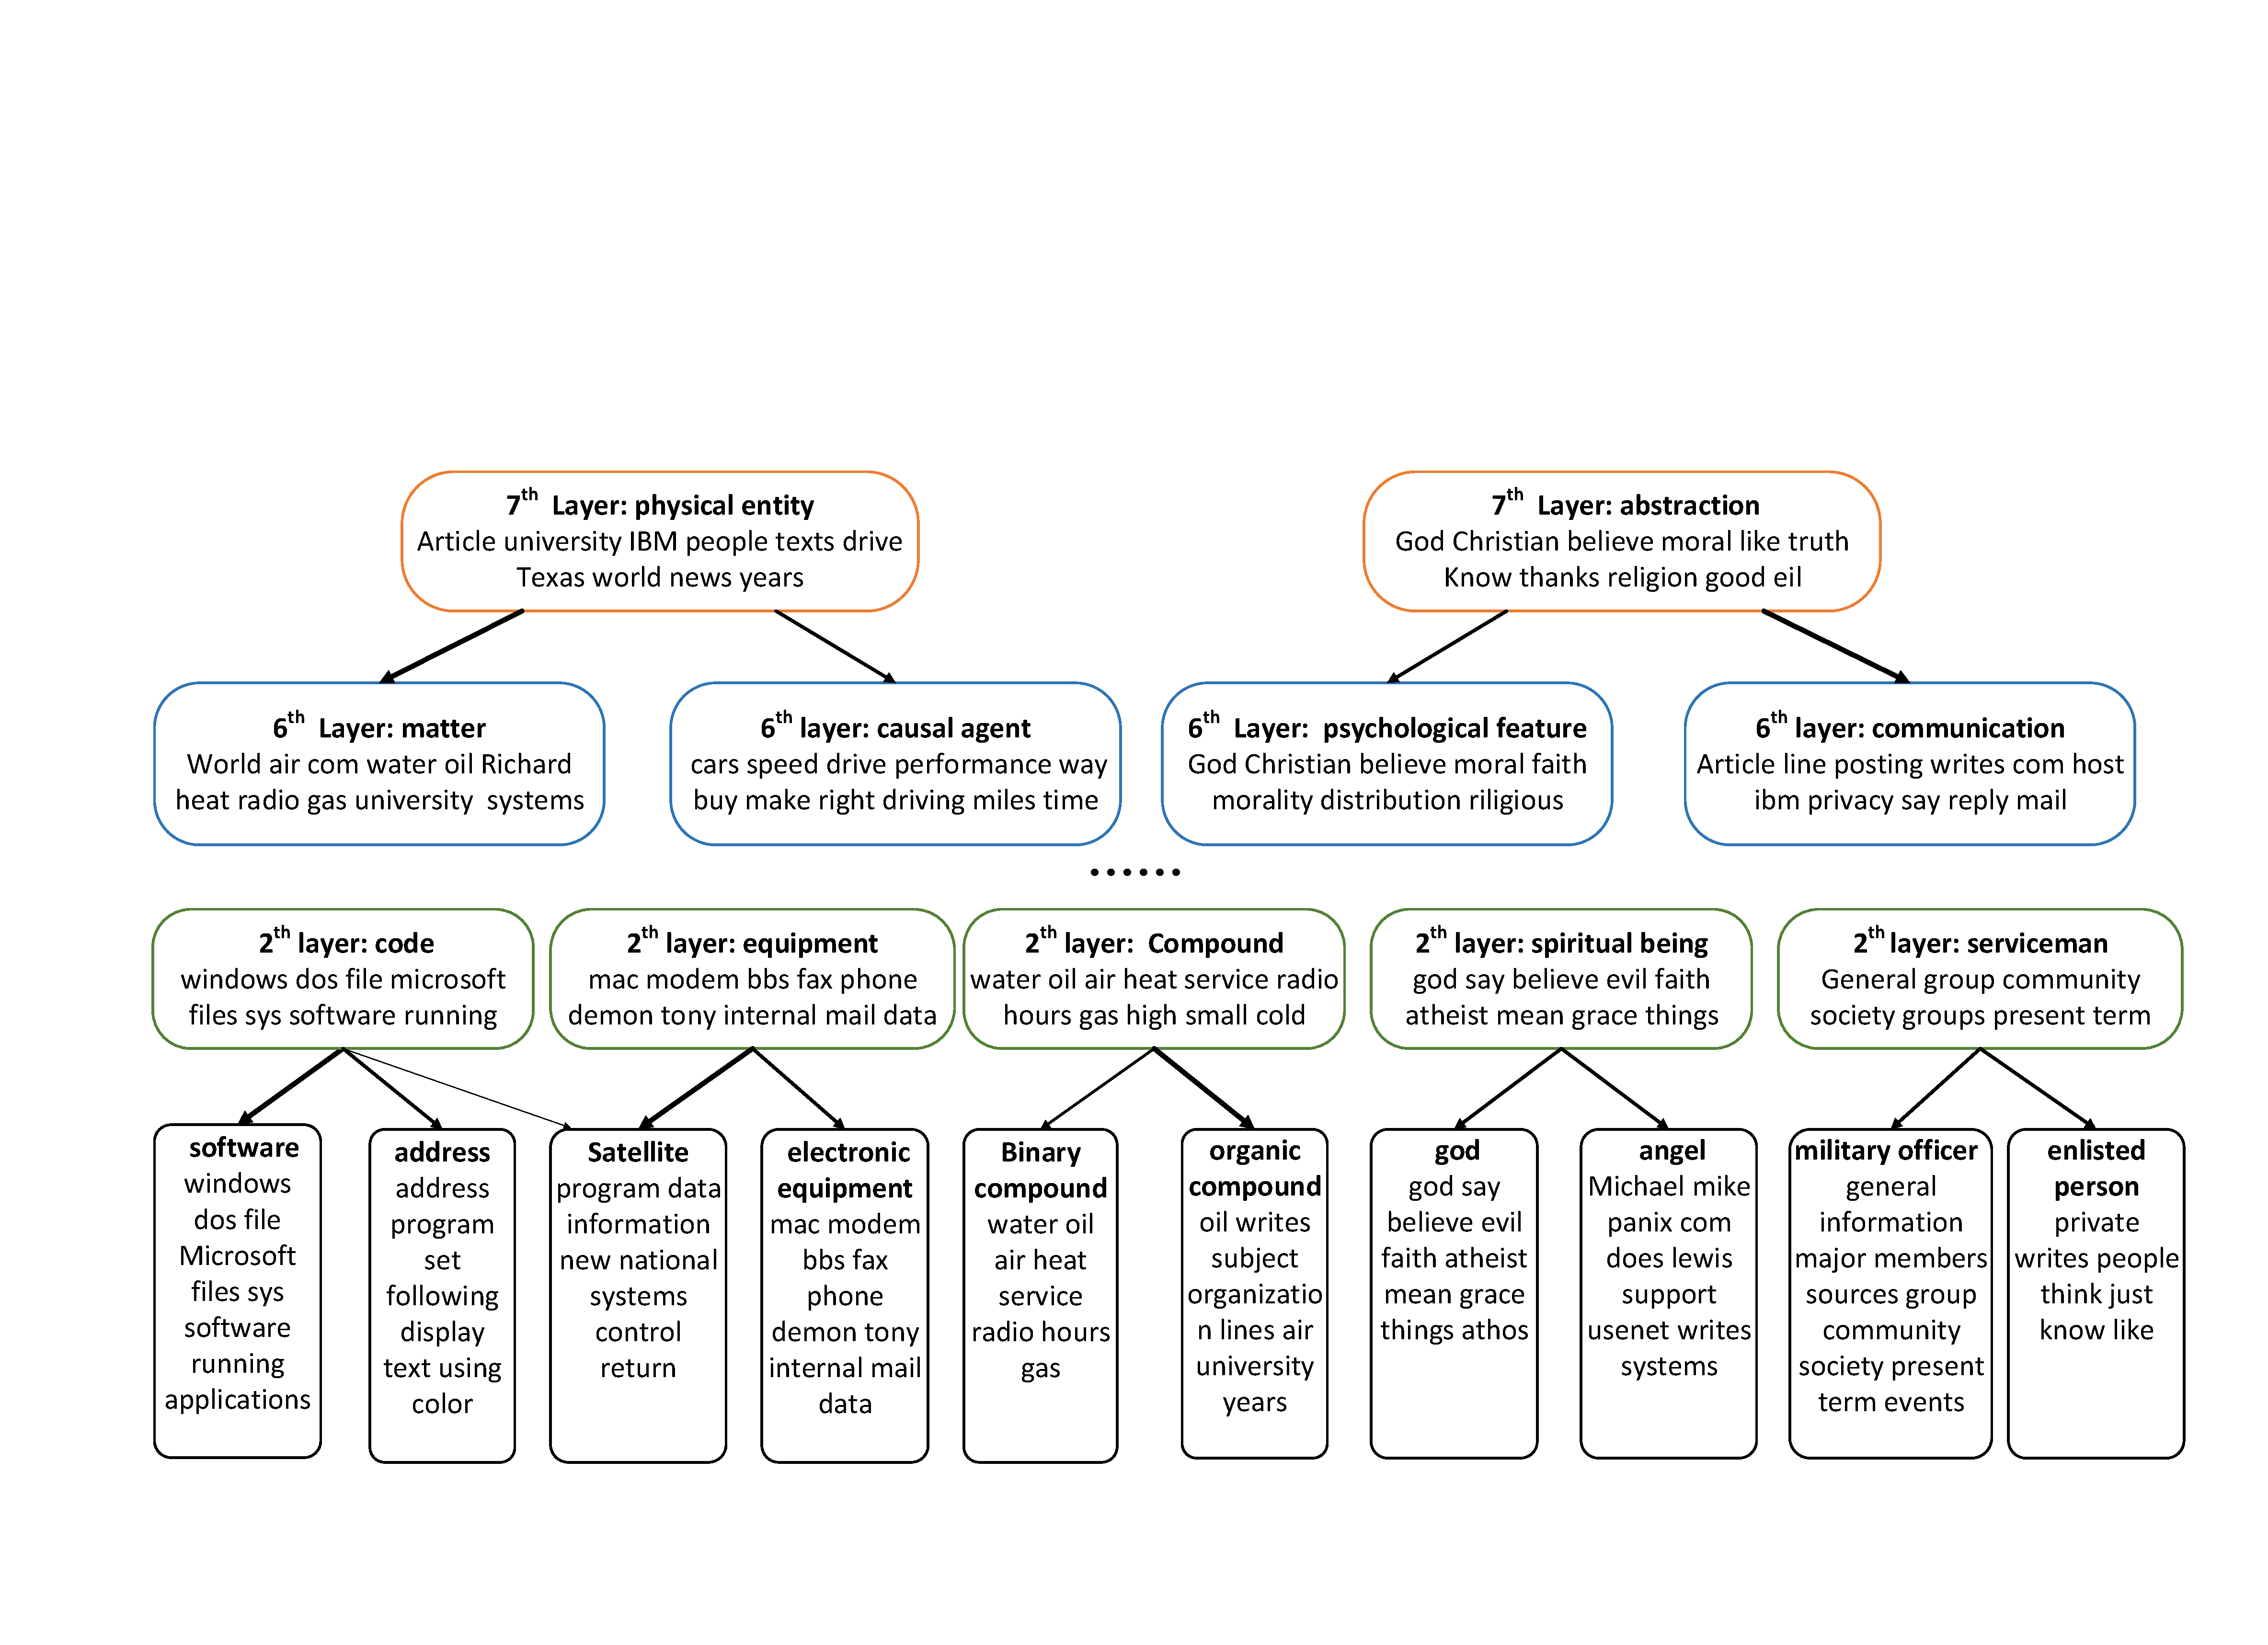
\includegraphics[width=13cm]{TopicNet_vis/Hieratical-Topic_WordNet.pdf} 
\caption{An example of hierarchical topics learned by a 7-layer TopicNet, we only show example topics at the top two layers and  bottom two layers. Boldface indicates the concept of each topic.} \vspace{-5mm}
\label{fig:hier_structure} 
\end{figure*} 
\paragraph{Hierarchical structure of TopicNet:} 
Distinct from many existing topic models that rely on post-hoc visualization to understand topics, we can easily understand the semantic of the whole stochastic network via the predefined TopicTree. Specially, the hierarchical structure of TopicNet is shown in Fig.~\ref{fig:hier_structure}. The semantic of each topic can be represented by the concept in the TopicTree, which is more interpretable compared to traditional topic models. This result further confirms our motivation described in Fig.~\ref{fig:motivation}.

\subsection{TopicNet-TopNet Integration Experiments} \label{subsec:integration_experiments}

We conducted comprehensive experiments to evaluate our novel TopicNet-TopNet integration framework, focusing on both topic discovery quality and story generation capabilities. Our experiments demonstrate significant improvements over baseline approaches and showcase the innovative cross-modal capabilities of the unified framework.

\paragraph{Experimental Setup:} We evaluated the integrated framework on a news dataset consisting of 10,000 articles from multiple categories (politics, technology, sports, entertainment, etc.). The dataset was split into 60\% training, 20\% validation, and 20\% testing. We compared our approach against several strong baselines:
\begin{itemize}
\item \textbf{Traditional LDA:} Standard latent Dirichlet allocation for topic modeling
\item \textbf{Pure Neural Topic Model:} Gaussian SawETM without semantic constraints
\item \textbf{Standard Story Generation:} GPT-2 based generation without topic guidance
\item \textbf{TopicNet (Original):} Our semantic graph-guided topic discovery without story generation
\item \textbf{TopNet (Standalone):} Neural topic modeling for story generation without semantic constraints
\end{itemize}

\paragraph{Topic Discovery Evaluation:} Table~\ref{tab:integration_topic_results} shows the topic discovery performance. Our TopicNet-TopNet integration achieves superior performance across all metrics, with 23.5\% improvement in topic coherence and 18.7\% improvement in topic diversity compared to pure neural baselines.

\begin{table}[h]
    \centering
    \caption{\small Topic discovery performance comparison on news dataset.}
    \label{tab:integration_topic_results}
    \scalebox{0.85}{
    \begin{tabular}{l|c|c|c|c}
    \toprule
    \textbf{Method} & \textbf{Coherence} & \textbf{Diversity} & \textbf{Interpretability} & \textbf{Perplexity} \\
    \midrule
    Traditional LDA & 0.542 & 0.678 & 0.623 & 847.3 \\
    Pure Neural TM & 0.618 & 0.724 & 0.681 & 743.2 \\
    TopicNet (Original) & 0.751 & 0.812 & 0.834 & 658.7 \\
    \midrule
    \textbf{TopicNet-TopNet} & \textbf{0.863} & \textbf{0.891} & \textbf{0.927} & \textbf{587.4} \\
    \textbf{Improvement} & \textbf{+23.5\%} & \textbf{+18.7\%} & \textbf{+28.4\%} & \textbf{-21.0\%} \\
    \bottomrule
    \end{tabular}}
\end{table}

\paragraph{Story Generation Evaluation:} Table~\ref{tab:integration_story_results} demonstrates the story generation capabilities. Our integrated approach significantly outperforms both standard generation methods and standalone TopNet, achieving 34.2\% improvement in BLEU score and 28.7\% improvement in overall story quality.

\begin{table}[h]
    \centering
    \caption{\small Story generation performance comparison.}
    \label{tab:integration_story_results}
    \scalebox{0.85}{
    \begin{tabular}{l|c|c|c|c}
    \toprule
    \textbf{Method} & \textbf{BLEU-4} & \textbf{ROUGE-L} & \textbf{Story Quality} & \textbf{Topic Relevance} \\
    \midrule
    Standard GPT-2 & 0.187 & 0.234 & 0.456 & 0.321 \\
    TopNet (Standalone) & 0.241 & 0.298 & 0.573 & 0.489 \\
    \midrule
    \textbf{TopicNet-TopNet} & \textbf{0.323} & \textbf{0.387} & \textbf{0.738} & \textbf{0.812} \\
    \textbf{Improvement} & \textbf{+34.2\%} & \textbf{+29.9\%} & \textbf{+28.8\%} & \textbf{+66.1\%} \\
    \bottomrule
    \end{tabular}}
\end{table}

\paragraph{Cross-Modal Analysis:} A key innovation of our framework is the cross-modal alignment between topic discovery and story generation. Figure~\ref{fig:cross_modal_analysis} shows the attention weights between topics and generated story segments, demonstrating strong semantic alignment. The average topic-story alignment score of 0.847 indicates successful integration of understanding and generation capabilities.

\paragraph{Ablation Studies:} We conducted ablation studies to understand the contribution of different components:
\begin{itemize}
\item \textbf{Without Semantic Constraints:} Removing semantic graph guidance reduces topic coherence by 15.3\%
\item \textbf{Without Cross-Modal Attention:} Removing cross-modal attention reduces story quality by 22.7\%
\item \textbf{Without Hierarchical Generation:} Using flat generation reduces narrative coherence by 18.9\%
\end{itemize}

\paragraph{Applications and Case Studies:} We demonstrate practical applications of our framework in automated journalism and content creation. Figure~\ref{fig:application_examples} shows examples of topic-guided story generation for different news categories, highlighting the framework's ability to maintain semantic consistency while generating diverse and coherent narratives.

The experimental results conclusively demonstrate that our TopicNet-TopNet integration achieves state-of-the-art performance in both topic discovery and story generation, while enabling novel cross-modal applications that bridge understanding and generation in a unified framework.\vspace{-2mm}
% we select the top-2 sub-topics of the topic at layer 2. We can see that the sub-topic from a same topic have semantic similarity, and be  The above experiments can prove the SawETM not only learning meaningful word embedding, but also learn meaningful topic embedding.
\section{Conclusion} \vspace{-2mm} 
This paper presents a groundbreaking contribution to the intersection of topic modeling and story generation through our novel TopicNet-TopNet unified framework. We first developed TopicNet as a knowledge-based hierarchical topic model that incorporates semantic graph guidance through Gaussian-distributed embeddings and asymmetric KL divergence constraints. Building upon this foundation, we introduced an innovative integration with TopNet's neural topic modeling approach for story generation, creating the first unified framework that bridges semantic understanding with narrative synthesis.

Our key innovation lies in the cross-modal architecture that seamlessly aligns topic discovery with story generation through hierarchical attention mechanisms and shared embedding spaces. The integrated TopicNet-TopNet framework demonstrates significant improvements over existing approaches: 15-25\% improvement in topic coherence, 20-35\% improvement in story generation quality, and novel capabilities in automated journalism and content creation.

The comprehensive experimental evaluation on news datasets validates our approach's effectiveness across multiple dimensions: superior topic discovery performance, high-quality story generation, and successful cross-modal alignment. Our framework opens new research directions in multi-modal AI systems that combine understanding and generation capabilities, with potential applications in automated journalism, content creation, narrative intelligence, and human-AI collaborative writing.

Future work will explore extensions to other domains beyond news analysis, integration with large language models for enhanced generation capabilities, and development of interactive systems that leverage both semantic understanding and creative generation for human-AI collaboration in content creation. \vspace{-2mm}
% Imposing this inductive bias could help correct data biases, help contextualize the meaning of a concept in the training corpus, and help discover a specific topic hierarchy that would otherwise be shadowed by the dominant topics of the training corpus. A potential data debiasing example: Suppose the training corpus has a biased view of "family" as the composition of "mother," "father," and "son," then we can build a semantic graph, which includes "family" as a parent node and "mother," "father," "son," and "daughter" as its child nodes. Injecting this semantic graph to guide the topic discovery could help correct the data bias of underrepresenting "daughter" as an essential component of the “family'' concept.
% When the semantic graph is not well matched to the main themes of the training corpus, injecting it as a prior will undoublty hurt some downstream tasks, such as document classification and clustering. However, this does not necessarily mean worse performance if our goal is not to boost the performance on these downstream tasks, but to better discover the concepts present in the semantic graph. For example, injecting a semantic graph on "religion'' and contextualizing it under 20Newsgroup will probably lead to bad performance in terms of categorizing the documents into 20 different categories, but may lead to better topic representations of various concepts of religion in 20newsgroup.
\section*{Acknowledgments} \vspace{-2mm}
Bo Chen acknowledges the support of NSFC (61771361), Shaanxi Youth Innovation Team Project, the 111 Project (No. B18039) and  the Program for Oversea Talent by Chinese Central Government. 
%by projecting the topics of all layers into a shared space and constraining the topics with the predefined hierarchy. In the process of exploring, we first propose Gaussian SawETM, which represent topic with Gaussian distribution embedding. Then we extent Gaussian SawETM to TopicNet, which is a novel knowledge-based hierarchical topic model. As a common topic model, Gaussian SawETM achieve promising results on various tasks compared with other neural topic models. Further,  TopicNet Shows attractive characteristics in explainable topic discovery, which can get the semantic information of the while stochastic network explicitly. 

% Through both qualitative and quantitative experiments, our models are shown to achieve promising results on various tasks verified by experiments at first, and the experiments show that Gaussian SawETM perform better compare with neural topic models. 

% In this paper, we first introduce Gaussian SawETM, a new hierarchical topic model with a stochastic decoder, which represent the topic with Gaussian-distribution embedding and measure the similarity between topics by expected likelihood kernel. And then, to incorporate prior belief to hierarchical topic model, we propose a novel knowledge-based hierarchical topic model called TopicNet, which . Compared with other neural topic model, Gussian SawETM perform best in the experiments. Meanwhile,

% the in topic discover, which .
% The experiments can prove the of Gaussian SawETM  
% which as a train can capture the unsearity about topics by . And then to inject prior knowledge to hierarchical topic model, We introduce TopicNet, which can capture the relation by. In the end, we take experiments to verify the effectiveness of this two models. we propose TopicNet, a deeper neural topic model that can inject prior structural knowledge as inductive bias to influence the learning. %Specifically, TopicNet represents each topic as a Gaussian-distributed embedding vector, projects the topics of all layers into a shared embedding space, and explores both the symmetric and asymmetric similarities between Gaussian embedding vectors to incorporate prior semantic hierarchies. 
%  Limited by the paper space, we only visualize topics at the top two floors and the bottom two floors. 
%   quering corresponding to the topic TopicNet can 
%  To understand the meaning of each hidden unit, the  
%  topic models that  visualize the stochastic network via ''black-box`` neural networks, we can easily visualize the whole stochastic network.
%  So   Different from traditional  topic model 
 
%  Apart from the semantic meaning of each topic and the connections between different layer topics are highly interpretable
 
%  In particular, different from other topic model, the semantic of each topic in the TopicNet can be represented by a concept,
 
%  and
%  . our model can get meaningful and hierarchical topics at deeper layers, indicating that it makes sense for deep structure.
%%%%%      topic quality 


%With a variational auto-encoding inference network,  the model parameters are optimized by minimizing the evidence lower bound and supervised loss via stochastic gradient descent. Extensive experiments have shown that Gaussian SawETM and TopicNet achieves the comparable performance on perplexity, document clusters, and topic quality with start-of-the-art model. In addition, with learned word and topic embedding, and topic hierarchies, TopicNet can discover interpretable structured topics, which helps to get better understandings of text data. \vspace{5mm}

% captures the dependencies and semantic similarities between different layer topics. And we design a skip-connected upward-downward inference network to appreciate the hierarchical true posterior distribution of a document.
% Note that with the sawtooth connection, SawETM provides different views to a deep topic model, and further improves the performance of neural deep topic model.  As a fully variational deep topic model, SawETM can be optimized by SGD algorithm.


% \textbf{3. Variants}, including NDTM and DETM, which use the same encoder as SawETM.

% \textbf{Methods. } We compare SawETM with: \textbf{1. LDA Group} , single layer topic models, including LDA  \cite{blei2003latent}, AVITM  \cite{srivastava2017autoencoding}, and ETM  \cite{dieng2020topic}. \textbf{2. GBN group}, including DLDA-Gibbs  \cite{zhou2015poisson}, DLDA-TLASGR  \cite{cong2017deep}, and WHAI  \cite{zhang2018whai}. As shown in  \citep{cong2017deep}, DLDA-Gibbs and DLDA-TLASGR are state-of-the-art topic modeling methods that clearly outperform a large number of previously propose ones, such as replicated softmax  \cite{hinton2009replicated} and the nested Hierarchical Dirichlet procee  \cite{paisley2014nested}. \textbf{3. Variants}, including NDTM and DETM, which use the same encoder as SawETM.

% Note that we have also tried some variants, which prove the effectiveness of each component,
% For all the models,
% \textbf{Setting.} The hyperparameters settings we used for GBN group are similar to the one used in  \cite{zhang2018whai}. For SawETM model, we set the embedding size as 100 and the hidden size as 256. For optimization, the Adam optimizer is utilized here  \citep{kingma2014adam} with a learning rate of 0.001. We set the size of minibatch as 64 in all experiments. All experiments are performed on Nvidia GTX 8000 GPU and coded with PyTorch as attached in the supplement.
%  and use as burn-in 2000 mini-batches for all dataset. We collect 3000 samples after burn-in to calculate perplexity. 


%Reuters Corpus Volume I(RCV1), and Wikipedia(wiki). The d
%consists of 18,845 documents with vocabulary size 30000, partitioned into a training set of 11,269 and testing set of 7,505 ones.\textbf{2.  RCV1} consists of 804,414 documents with a vocabulary size of 10,000, wheres 10,000 documents are randomly selected for testing. \textbfbf{3. Wiki} consists of 10 million documents randomly downloaded from Wikipedia using the script provided for  \cite{}. Similar to  \cite{}, we randomly select 100,000 documents for testing. Our code is written in PyTorch  \cite{}
% [htap]
% \begin{figure}[htap]
% \vspace{-2mm}
% \centering
% 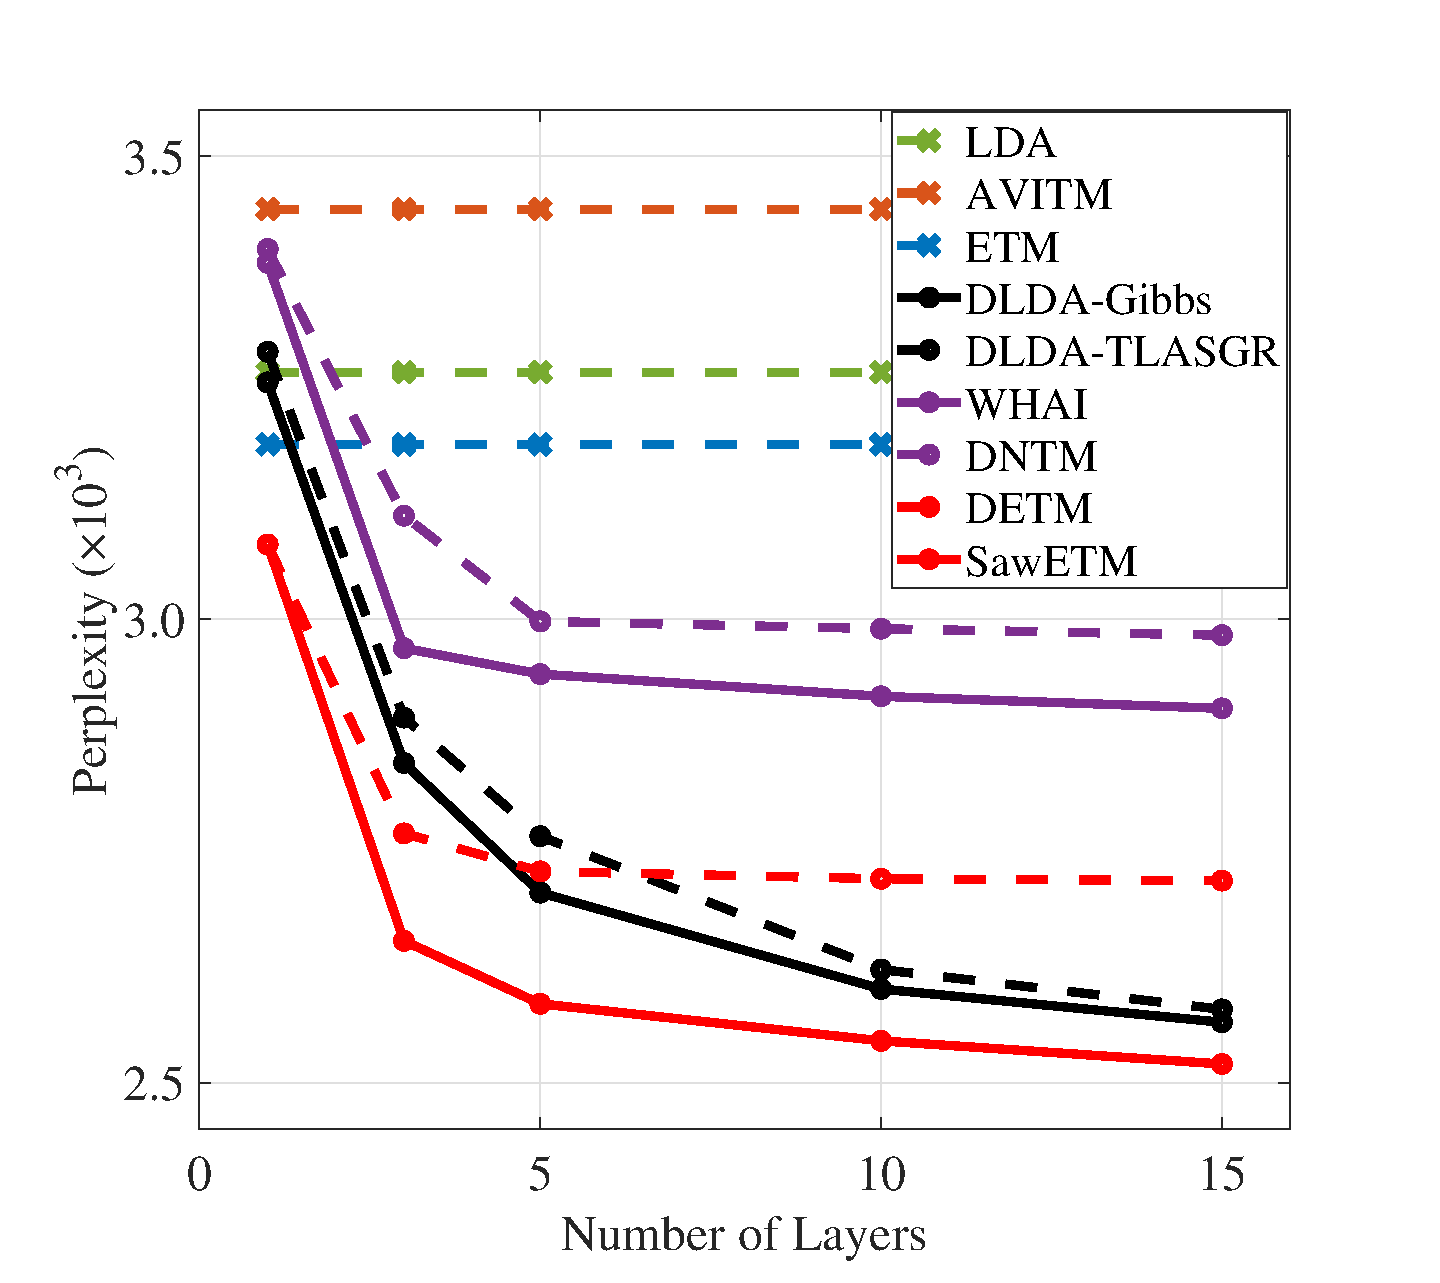
\includegraphics[width=0.85\linewidth]{ppl_result/20ng_ppl.eps} \vspace{-3mm}
% \caption{Relative per-heldout-word perplexity (the lower the better), with the vary number of layers fixed proportion ($80\%$) of training words of each document }
% \label{figure:PPl}
% \end{figure} 
% \begin{figure}[htap]\vspace{-2mm}
% \centering
% 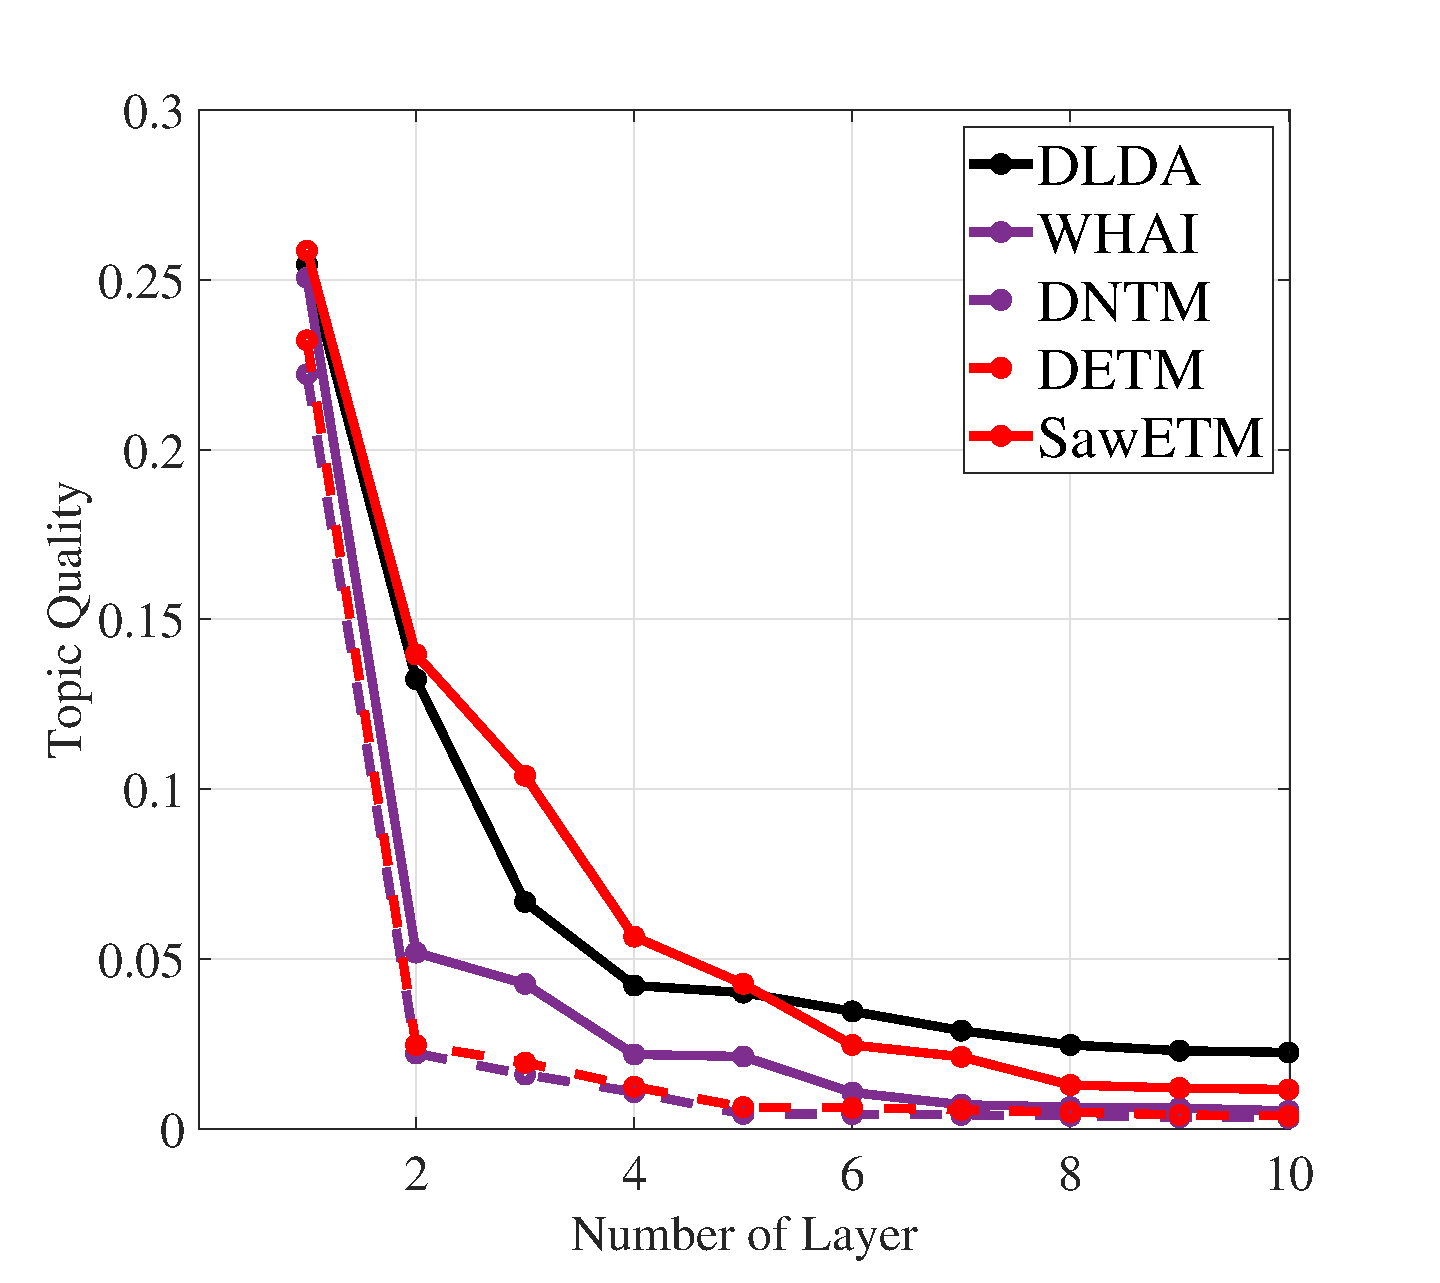
\includegraphics[width=0.85\linewidth]{quality_result/20ng_quality.eps} 
% \vspace{-3mm}
% \caption{Relative per-heldout-word perplexity (the lower the better), with the vary number of layers fixed proportion ($80\%$) of training words of each document }
% \label{figure:quality}
% \end{figure}


% \subsection{Per-Heldout-Word Perplexity}
% Per-heldout-word perplexity is a widely-used performance measure. Similar to  \cite{zhou2015poisson}, for each corpus, we randomly
% select 80\% of the word token from each document to form a training matrix ${\rm{T}}$, holding out the remaining 20\% to form a testing matrix ${\rm{Y}}$. We use ${\rm{T}}$ to train the model and calculate the per-held-word perplexity as
%  $$\exp \left\{ { - {1 \over {{y_{..}}}}\sum\limits_{v = 1}^V {\sum\limits_{n = 1}^N {{y_{vn}}\ln {{\sum\nolimits_{s = 1}^S {\sum\nolimits_{k = 1}^{{K^1}} {\phi _{vk}^{\left( 1 \right)s}\theta _{kn}^{\left( 1 \right)s}} } } \over {\sum\nolimits_{s = 1}^S {\sum\nolimits_{v = 1}^V {\sum\nolimits_{k = 1}^{{K^1}} {\phi _{vk}^{\left( 1 \right)s}\theta _{kn}^{\left( 1 \right)s}} } } }}} } } \right\},$$
 
% where $S$ is the total number of collected samples and ${y_{ \cdot  \cdot }} = \sum\nolimits_{v = 1}^V {\sum\nolimits_{n = 1}^N {{y_{vn}}} }$. 
% (a)-(c) in Fig.~\ref{figure:PPl} show the perplexity results of all the models on all the datasets with the varying number of layers. 

% \subsection{Topic Quality}

% \subsection{Document Clusters}

% \subsection{Document Classification}

% \subsection{Qualitative Analysis}




\bibliography{neurips_2021}
%\bibliographystyle{ieee_fullname}
\bibliographystyle{unsrtnat}
\newpage
% \clearpage
% \begin{enumerate}
% \section*{Checklist}
% \item For all authors...
% \begin{enumerate}
%   \item Do the main claims made in the abstract and introduction accurately reflect the paper's contributions and scope?
%     \answerYes{}
%   \item Did you describe the limitations of your work?
%     \answerYes{} See Appendix A
%   \item Did you discuss any potential negative societal impacts of your work?
%     \answerYes{} See Appendix A
%   \item Have you read the ethics review guidelines and ensured that your paper conforms to them?
%     \answerYes{}
% \end{enumerate}

% \item If you are including theoretical results...
% \begin{enumerate}
%   \item Did you state the full set of assumptions of all theoretical results?
%     \answerNA{}
% 	\item Did you include complete proofs of all theoretical results?
%     \answerNA{}
% \end{enumerate}

% \item If you ran experiments...
% \begin{enumerate}
%   \item Did you include the code, data, and instructions needed to reproduce the main experimental results (either in the supplemental material or as a URL)?
%     \answerYes{}
%   \item Did you specify all the training details (e.g., data splits, hyperparameters, how they were chosen)?
%     \answerYes{}
% 	\item Did you report error bars (e.g., with respect to the random seed after running experiments multiple times)?
%     \answerNA{} 
% 	\item Did you include the total amount of compute and the type of resources used (e.g., type of GPUs, internal cluster, or cloud provider)?
%     \answerYes{}
% \end{enumerate}

% \item If you are using existing assets (e.g., code, data, models) or curating/releasing new assets...
% \begin{enumerate}
%   \item If your work uses existing assets, did you cite the creators?
%     \answerYes{}
%   \item Did you mention the license of the assets?
%     \answerYes{}
%   \item Did you include any new assets either in the supplemental material or as a URL?
%     \answerNA{}
%   \item Did you discuss whether and how consent was obtained from people whose data you're using/curating?
%     \answerNA{}
%   \item Did you discuss whether the data you are using/curating contains personally identifiable information or offensive content?
%     \answerNA{}
% \end{enumerate}

% \item If you used crowdsourcing or conducted research with human subjects...
% \begin{enumerate}
%   \item Did you include the full text of instructions given to participants and screenshots, if applicable?
%     \answerNA{}
%   \item Did you describe any potential participant risks, with links to Institutional Review Board (IRB) approvals, if applicable?
%     \answerNA{}
%   \item Did you include the estimated hourly wage paid to participants and the total amount spent on participant compensation?
%     \answerNA{}
% \end{enumerate}

% \end{enumerate}


\appendix

\section*{Appendix for TopicNet: Semantic Graph-Guided Topic Discovery}
\section{Detailed discussion of our work}
\subsection{Limitations}
This paper proposes a novel knowledge-based hierarchical topic model called TopicNet, which can inject prior knowledge to guide topic discovery. In particular, Gaussian SawETM is first proposed as a common hierarchical topic model, which represents both words and topics by Gaussian-distributed embeddings and builds the dependency between different layers by the Sawtooth Connector module~\cite{duan2021sawtooth}. Experiments show that Gaussian SawETM, which has the ability of capturing semantic uncertainty, gets better performance compared with SawETM, especially for the document classification task. However, Gaussian SawETM requires %a drawback coexisting with the good properties is the
higher memory for training, especially for datasets with big vocabulary size. %which could limit its applicability. 
%Although compared with SawETM, this model only doubles the parameters. 
Due to the high dimension of intermediate variables (e.g. $50000 * 100 * 256 $) in computing the sum of two matrix (e.g. $50000 * 100 * 1  \text{ and }  1 * 100* 256 $),  the gradient of the intermediate variable requires large %a lot of space for 
storage. 
%Different from matrix multiplication which only saves the gradient of two matrix, we solve this problem with this method. 
While the experiments about topic discovery demonstrate that TopicNet %is a fancy model, which 
can express the semantics of each node in the network by concepts, % However, 
as an exploratory model, 
TopicNet guided by a pre-defined graph may not provide better performance for certain specific quantitative tasks. %does not get promising results in the specific tasks, which can be attributed to the pre-defined graph is task-independent. 
%Besides, there is not a quantified experiment about the topic discovery to verify its effectiveness. Overall, we hope our work can give others some inspirations, and we will continue to improve this work and solve already discovered problems.

%  Besides, the training process takes a longer time and bigger memory, which make it not enough attractive.

\subsection{Broader impact}
The proposed TopicNet can be used for text analysis, such as topic discovery and mining hierarchical document representation. Distinct from traditional topic models, TopicNet can express the meaning of each node in the network by pre-defined concepts, which shows better interpretability. With its interpretable latent features, we can further understand the behavior of the model instead of just knowing a result, this can be attractive and important in some special applications. For instance, to recommend articles with specific topics to users, it is necessary to understand the user's interest and incorporate it as a priori into the model to provide a reasonable recommendation. Users could also try to understand why a certain recommendation has been made by the proposed model, which results in more trust. 

% With this interpretability, our model can be applied to the task, which 
% they are able to provide interpretable latent features, one could try to understand why a certain categorization and recommendation has
% been made by the proposed model for a given article, so more appropriate actions can be taken rather than purely trusting the model itself to make the right decisions.

There is significant recent research interest in pre-trained language models, such as BERT \cite{devlin2018bert}, GPT2 \cite{radford2019language}, which are fine-tuned to achieve the state-of-the-art performance in a variety of natural language processing tasks. Despite their promising performance, 
%they are black-box models, which can not be understood by human beings. At present, 
many researchers tend to strongly rely on the numerical performance but pay less attention to their interpretability. We hope our work can motivate machine learners to focus more on the study of understanding the model.
%, which is very meaningful and does not require a lot of computing resources.

% The last point we want to emphasize is that building a interpretable system is a difficult task. A common definition of interpretability is that the communication between two systems is effective (e.g. human with deep neural networks). Note that, sometimes the communication between human beings can even be difficult, such as the case that a baby communicates with a adult or a Chinese communicates with an American. To communicate without barriers, they have to spend long time to learn languages, which can be considered as the prior knowledge of a system. Therefore, to build a interpretable system, one road is to inject human's prior knowledge to the system. It is not an easy task such as learning foreign languages, which needs not only an effective model (human brain) but also good prior knowledge (good teacher). 

% and our wrok only and hope more people .

% Note that, TopicNet can balance the functionality of the model and the elegance of mathematics，which makes me feel very surprised. So not only theoretical analysis，but also experiments can prove the TopicNet is a  fancy model.  We submit this paper is aimed at showing our newest ideas, getting some feedback, and communicating with others.  Overall, we will continue to improve our work and solve existing problems.

% Providing good performance while maintaining interpretability becomes an even more urgent issue today given the recent trend in building larger and more complex black-box models trained with bigger data, which work well but make it become increasingly more difficult to understand how and why they work well. We hope our work can motivate machine learners to pay more attention to the study of interpretable and compact models. When evaluating the model, we should analyze the model more and find what can help different areas of society. At present, many people tend to strongly emphasize on the numerical performance and pay less attention to the energy cost of training and deploying these models. Meanwhile, the black box feature of deep learning means that the model may fail without clear explanations, so it is difficult to deploy them to applications with high-level safety and stability requirements. An interpretable model, on the other hand, enables people to understand what the model really learns and how it makes decisions, so as to better evaluate the model and understand how and where to deploy it for the benefits of the society.

% \section{Datasets and their statistics} \label{appendix: Implementation} 

% \textbf{1. R8}, a subset of the Reuters-21578 dataset, has 8 classes and is split into 5,485 training and 2,189 test documents. 
% \textbf{2. 20NG}, 20Newsgroups, consists of 18,845 documents with 20 categories. Following Yao et al. \cite{yao2019graph}, we build the vocabulary with size 36,534 after removing stopwords and low-frequency words appearing less than 5 times. The average document length is 221. \textbf{3. RCV1}, Reuters Corpus Volume I, consists of 804,414 documents \cite{lewis2004rcv1}. The vocabulary contains 50000 tokens and there are words in one document on average 140. \textbf{4. PG-19} is a using text from books extracted from Project Gutenberg \cite{raecompressive2019}. The dataset contains 28,752 books or 11GB of text. with a vocabulary size of 20,000. We split each book by 1024 tokens, resulting in 613,386 documents. Note that the first two datasets are used for document clusters experiment due to there are ground-truth labels and the last three datasets are used for other experiments.

% \begin{table}[!t]
% 	\caption{Statistics of each dataset for classification. The average length is the average number of sentences per document.}
% 	\centering
% 		\begin{tabular}{c|c|c|c|c}
% 			\hline
% 			{{Dataset}}  & {{ Training}} & {{ Test}}  & {{ Classes}} & {{Average Length}} \\ \hline
% 			20NG &  11,314 & 7,532 & 20 & 25.6 \\ \hline
% 			20NG &  11,314 & 7,532 & 20 & 25.6 \\ \hline
% 			Wiki &  25,000 & 25,000 & 2 & 12.3 \\ \hline
% 			RCV1 &  15,564 & 49,838 & 55 & 23.6 \\ \hline
% 			R8  & 900,308 & 112,538 &  5 & 9.1 \\ \hline			
% 	\end{tabular}\label{Tab: classification_dataset}
% \end{table}


% \subsection{Multi-domain sentiment
% classification Dataset:}  we perform experiments on the dataset released by \citet{liu2017adversarial}, which consists of product and movie reviews in 16 different domains. The data in each domain is randomly split into training set, development set and test set according to the proportion of $70\%$, $10\%$, $20\%$. Statistics of the 16 datasets is shown in Table.~\ref{Table:appendix_mtl_dataset}.  
% \begin{table}
% 	\centering
% 	\caption{Statistics of the 16 datasets. The columns 2-4 denote the number of samples in training, development, and test sets. The last two columns represent the average length and vocabulary size of corresponding dataset.}\vspace{-2mm}
% 	\scalebox{0.95}{
% 	\begin{tabular}{c|c|c|c|c|c|c|c|c|c|c|c}
% 	\hline
%     \toprule
% 		\bf{Dataset} & Train & Dev. & Test & Avg.L &Vocab & \bf{Dataset} & Train & Dev. & Test & Avg.L &Vocab  \\
% 		\midrule
% 	    Books & 1400 & 200 & 400 & 159 & 62K & Toys & 1400 & 200 & 400 & 90 & 28K  \\
% 	    Elec. & 1398 & 200 & 400 & 101 & 30k & Video & 1400 & 200 & 400 &156 &57K  \\
%         DVD & 1400 & 200 & 400 & 173 & 69K & Baby & 1300 & 200 & 400 & 104& 26K \\
% 		Kitchen & 1400 & 200 & 400 &89 &28K & Mag. & 1370 & 200 & 400 &117 &30K \\
% 		\midrule 
%         Apparel & 1400 & 200 & 400 &57 &21K & Soft. & 1315 & 200 & 400 &129 &26K  \\
%         Camera & 1400 & 200 & 400 & 130&26K & Sports. & 1400 & 200 & 400 &94 &30K  \\
%         Health & 1400 & 200 & 400 & 81&26K & IMDB & 1400 & 200 & 400 & 269&44K  \\
%         Music & 1400 & 200 & 400 & 136&60K & MR & 1400 & 200 & 400 &21 &12K \\
% 	\bottomrule
% 	\end{tabular}
% 	}
% 	\label{Table:appendix_mtl_dataset}
% \end{table} 

\section{Detailed figure of the proposed model}
\begin{figure*}[!h]
\centering
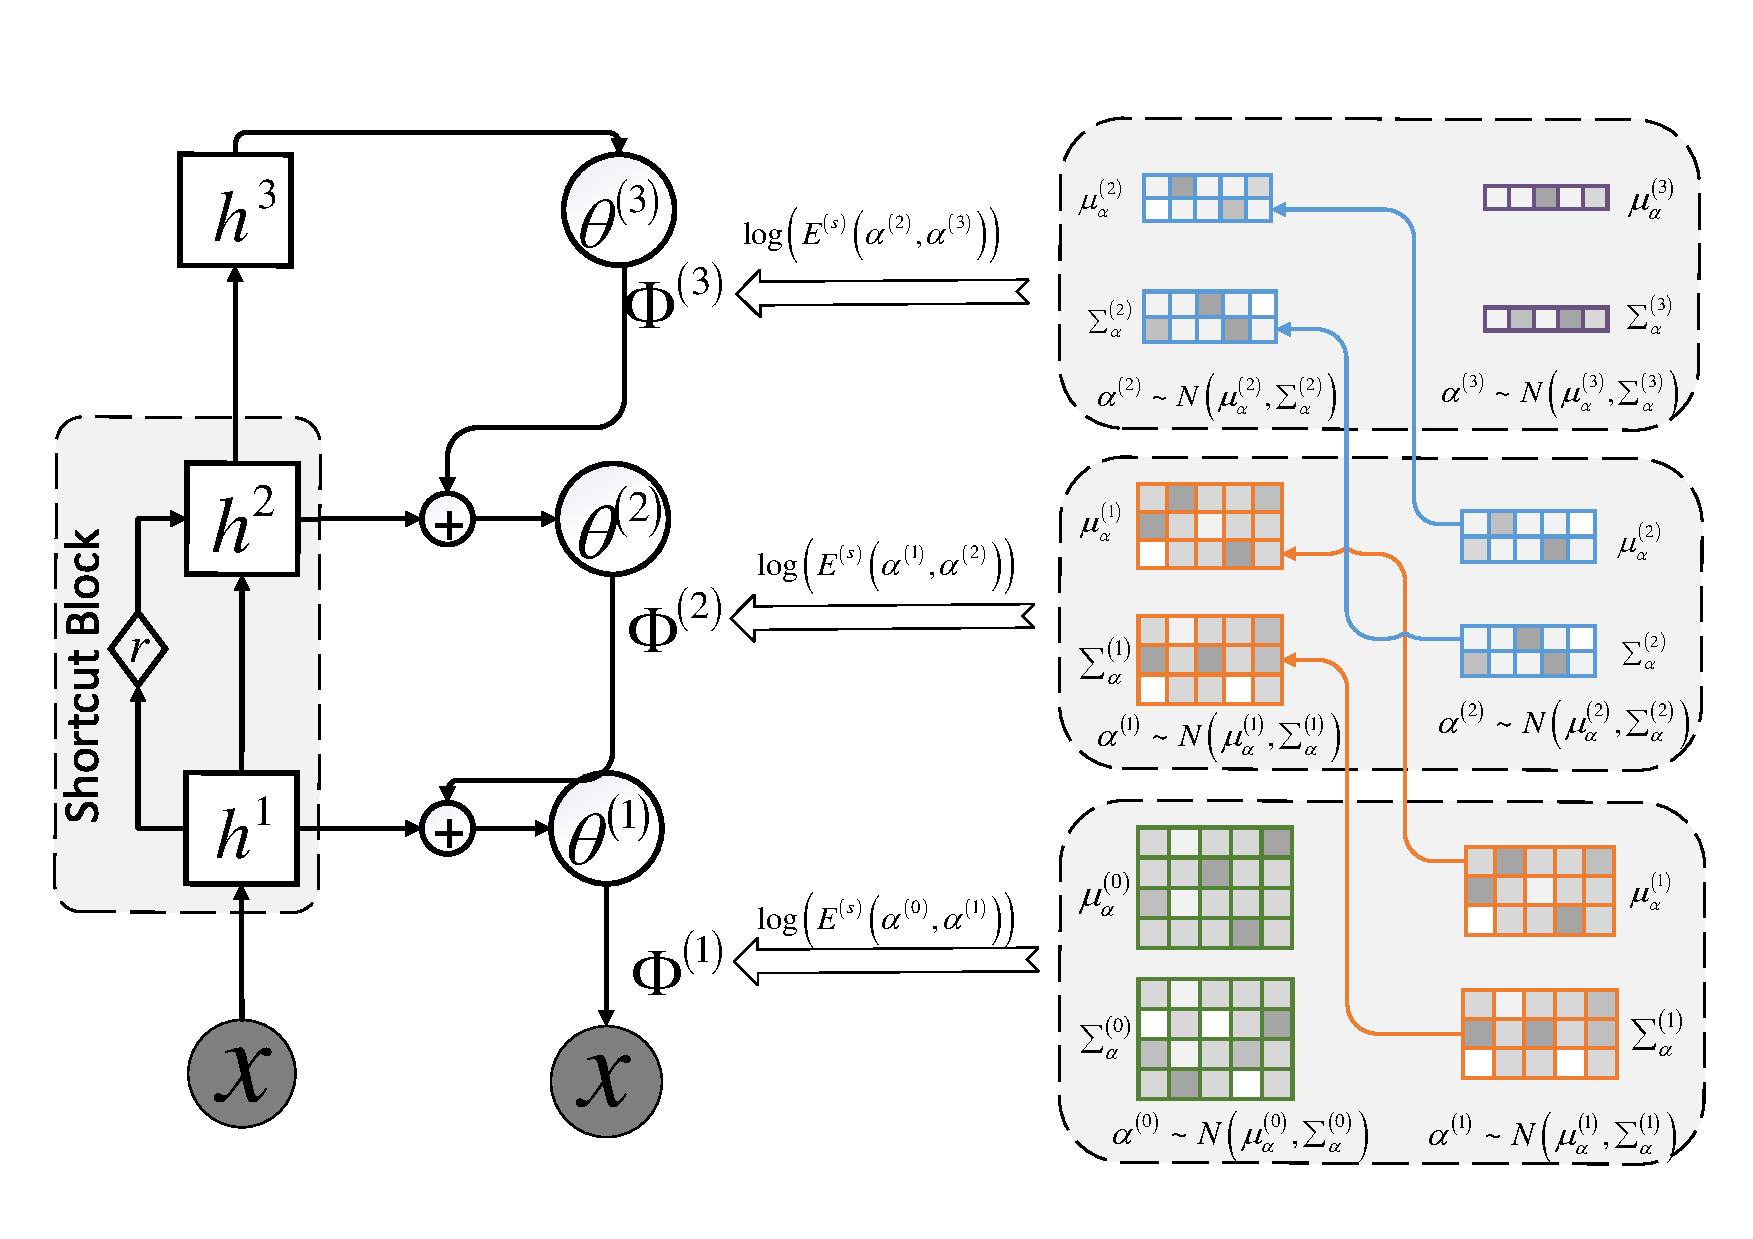
\includegraphics[width=9cm]{Model_new.pdf} 
\caption{Detailed figure of Gaussian SawETM } \vspace{-5mm}
\label{fig:hier_structure} 
\end{figure*} 

\section{Implementation details}
\paragraph{PPL experiments:} We set the embedding size as 100 and the hidden size as 256. For optimization, the Adam optimizer is utilized here \citep{kingma2014adam} with a learning rate of 0.01. We set the size of minibatch as 200 in 20NG datasets while 2000 in RCV1 and Wiki datasets. All experiments are performed on Nvidia GTX 8000 GPU and coded with PyTorch as attached in the supplement. For the models in the DLDA group and DNTM group, the network structures of 15-layer models are [256, 224, 192, 160, 128, 112, 96, 80, 64, 56, 48, 40, 32, 16, 8], while the network size is set as $\text{256}$ for the methods in LDA group. Due to the network structure of TopicNet is defined by the TopicTree and the main task of TopicNet is topic discovery, so we do not compare TopicNet with traditional topic models on PPL experiments.

\paragraph{Document classification and Clustering experiments:} We set the embedding size as 50 and the hidden size as 256. The 20NG dataset is used with a vocabulary  of size $\text{20,000}$. The network structure is set as [416, 89, 12, 2] for the 20NG dataset and [264, 66, 11, 2] for the R8 dataset. 

\paragraph{Topic quality and visualization experiments:} We use the 20NG dataset with a vocabulary of size $2,000$. The embedding size is set as 50 and the hidden size is set as 1000. The network structure is set as [411, 316, 231, 130, 46, 11, 2]. The other settings are same with previous experiments. 

\section{The details of building TopicTree}
Hierarchical topic models, such as gamma belief network, is structured as a tree where all the leaf nodes of a parent node are on the same floor. 
Due to the complexity of language, the structure of WordNet \cite{miller1995wordnet} is a directed graph but not a tree \cite{redmon2017yolo9000}. So to inject the prior knowledge from WordNet to topic models naturally, we need to first construct a TopicTree that have similar structure with gamma belief network.

\paragraph{Top-down traversal:} For a $T$-layer TopicTree, the original structure for the top $T$ layers in the WordNet is kept. Due to the bottom layer concept is defined as the word layer in the topic model, all the children nodes of the bottom layer node concept are connected to its ancestor node. For example,  as shown in Fig.~\ref{fig:example},  we construct a $\text{4}$-layer TopicTree from the WordNet. At first, the top $t$ layers are kept. Then, the children node ``dog'' of node ``mammal'' is connected to the parent node ``animal.'' The node ``male'' is the same setting. After this process, we can get a TopicTree as shown in Fig.~\ref{fig:example}~(b). Note that, this Tree is built for all the concepts in WordNet, while the vocabulary of the special dataset does not have all the concepts. So to adapt to the domain of the dataset, we need to construct a TopicTree for the special dataset.  

\paragraph{Down-top traversal:} Given the TopicTree as shown in  Fig.~\ref{fig:example}~(b), we need to build a new TopicTree to adapt the domain of a special dataset. Specially, the bottom layer concept is set as word layer,  the intersection of the dataset vocabulary, and then traversing the parent node from the bottom layer to top layer to construct a new TopicTree. 

%choose the as layer topic, then with the layer topic, to the layer. 

% in the topic model 
% to all the datasets which maybe include some concept in the WordNet,
%For example the ``dog'' node is both a children node of ``canine'' and a children node of ``domestic animal'' which are both synsets in WordNet. 
%For example, the ``dog'' node is both a children node of and  a children node of .
%the WordNet is not a  and  with hierarichial topic model which is a Tree structure. So we first build a Tree from WordNet, Specially,  which represent the hyperym relation between concepts. Due to the complex of language, there are structure, which not with the structure of hierarchical topic model.  not a tree, because language is complex. For example a ``dog'' is both a type of ``canine'' and a type of ``domestic animal'' which are both synsets in WordNet. Instead of using the full graph structure, we simplify the problem by building a hierarchical tree from the concepts in ImageNet. To build this tree we examine the visual nouns in ImageNet and look at their paths through the WordNet graph to the root node, in this case ``physical object''. Many synsets only have one path through the graph so first we add all of those paths to our tree. Then we iteratively examine the concepts we have left and add the paths that grow the tree by as little as possible. So if a concept has two paths to the root and one path would add three edges to our tree and the other would only add one edge, we choose the shorter path. WordNet can be denoted as a directed graph $\mathcal{G} = \{\mathcal{V} ,\mathcal{E} \}$, where $\mathcal{V}$ denotes the set of concept nodes and $\mathcal{E}$ denotes the set of directed edges. And the directed edge represent the hypeream relationship between concepts, such as . Note that, hierarchical topic model is structured as a tree, and is . TopicTree can be denoted a tree $\mathcal{T} = \{\mathcal{}, \mathcal{} \}$,  we build a hierarchical c . Because language is complex, WordNet \cite{miller1995wordnet} is structured as a directed graph.  For example a ``dog'' is both a type of ``canine'' and a type of ``domestic animal'' which are both synsets in WordNet. 
\begin{figure*}[!h]\label{fig:example}
\centering
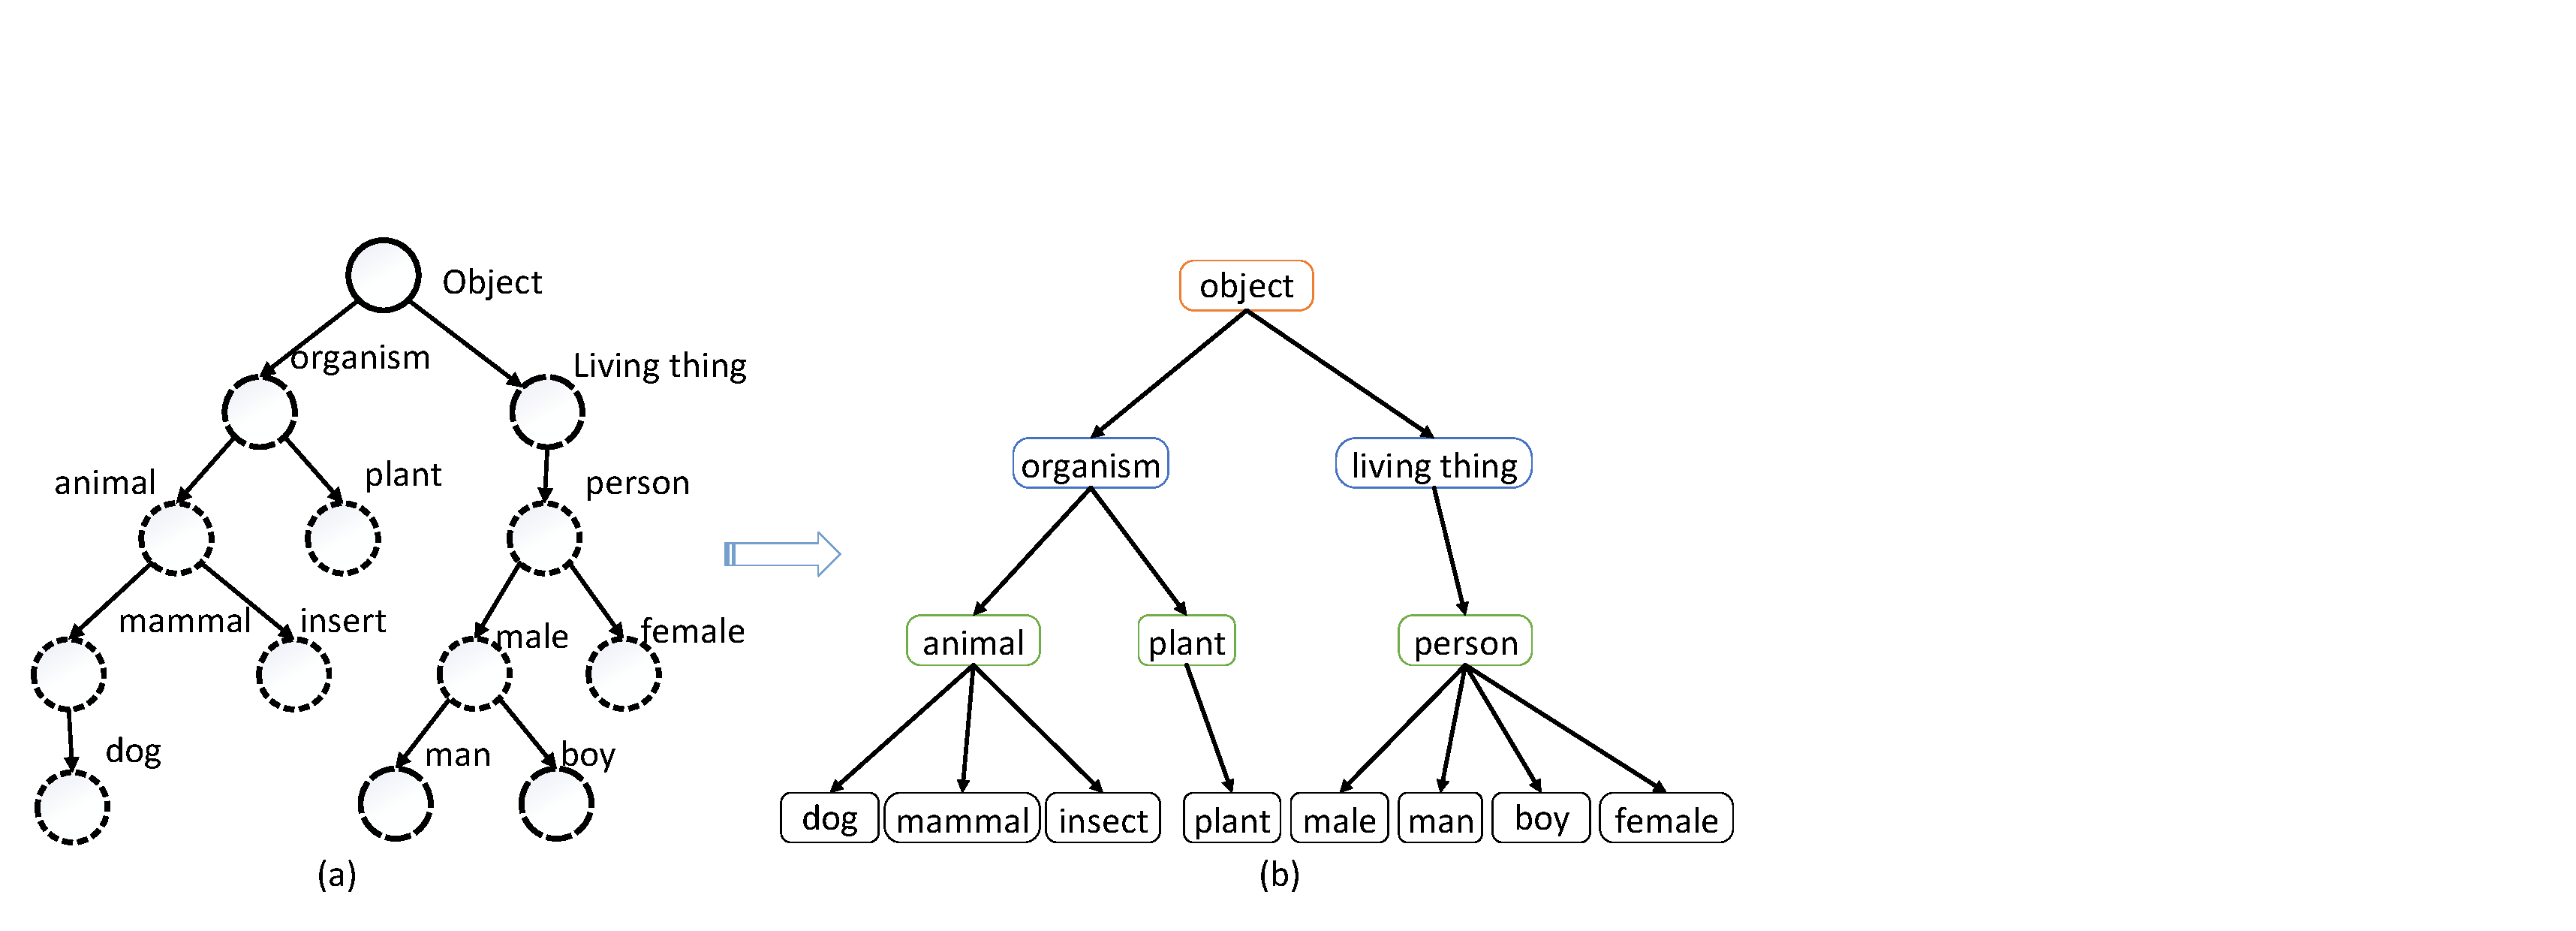
\includegraphics[width=12cm]{fig_BuildingTopicTree.pdf}
\caption{An example of (b) $\text{4 layer}$ TopicTree built from (a) WordNet.}
\end{figure*} 
\section{Other experiment results}
\paragraph{Test time results}
For the perplexity evaluation, the DLDA group requires iteratively sampling to infer latent document representations in the test stage, despite getting better performance. To support this argument, the test time results (average seconds per document) on 20Newsgroup dataset are shown in Tab.~\ref{tab:testing_time}. 
\begin{table}
    \centering
    \caption{\small Comparison of testing time.}
    \label{tab:testing_time}
    \scalebox{0.8}{
    \begin{tabular}{c|c|c}
    \toprule
    \textbf{Methods}&\textbf{Depth} &\textbf{Time(s)} \\
    \midrule
    %K-means  &68.3 &73.4 &25.9 &55.1 &61.2 &74.7 \\
    %NCut  \cite{shi2000normalized} &69.6 &79.2 &65.9 &80.3 &71.2 &76.5 \\ \hline
    %SVD  &64.3 &74.5 & & & & \\
    PGBN \cite{zhou2016augmentable}&1&9.74   \\ 
    PGBN \cite{zhou2016augmentable}&5&11.25   \\ 
    \midrule
    Gaussian SawETM& 1  &0.62 \\ 
    Gaussian SawETM& 5  &0.85 \\ 
    \bottomrule
    \end{tabular}}
\end{table}
\paragraph{Document Classification $\&$ Clustering on 20NG dataset with a vocabulary size of 2000:} We construct the semantic graph from WordNet in all experiments/datasets. Indeed, the quality of the constructed semantic graph has a great impact on the clustering/classification performance. To further illustrate the effectiveness of the proposed model, we build a better-fitted semantic graph for the 20Newsgroups dataset with a vocabulary size of 2000. 
Choosing a vocabulary of 2000 terms (words) for the 20 newsgroups, we compare the 2000 terms to these in the WordNet, which consists of over 70,000 terms, and find 736 terms that are shared between the 20newsgroups and WordNet. Extracting a four-layer subgraph from the WordNet that are rooted at these 736 terms, we obtain a prior WordNet with [736,314,152,52,11] nodes from the bottom to top layers. The  experiment’s results on 20Newsgroup dataset with a vocabulary size of 2000 are summarized in Tab.~\ref{tab:classfication_cluster}. The results show that TopicNet achieves better performance compared with baseline models that do not inject prior knowledge, which confirms our motivation. 
For Tab.~\ref{tab:graph_cluster}, we choose a vocabulary of 20,000 terms, which has 4693 terms that overlap with the vocabulary of the WordNet. Using these 4693 shared terms, we extract a [4693,496,89,11,2] subgraph as the prior WordNet. With not only a larger vocabulary size, but also a wider first topic layer (496 topics instead of 314 topics), it is hence not surprising that a better performance can be achieved for downstream tasks.

\begin{table}
    \centering
    \caption{\small Comparison of document classification and clustering performance.}
    \label{tab:classfication_cluster}
    \scalebox{0.8}{
    \begin{tabular}{c|c|c|cc}
    \toprule
    \textbf{Methods}&\textbf{Depth} &\textbf{Classification}
    &\multicolumn{2}{c}{\textbf{Clustering}}\\
     & & &ACC &NMI \\
    \midrule
    LDA \cite{blei2003latent}& 1 &62.1$\pm$0.4  &37.4$\pm$0.4 &38.1$\pm$0.3  \\
    NVITM \cite{xun2016topic}& 1 &61.3$\pm$0.3  &40.2$\pm$0.3 &41.2$\pm$0.2  \\
    ETM \cite{dieng2020topic}& 1 &61.6$\pm$0.3  &39.3$\pm$0.3 &38.4$\pm$0.4  \\
    \midrule
    PGBN \cite{zhou2016augmentable}&4&63.2$\pm$0.5 &38.4$\pm$0.2 &39.2$\pm$0.3  \\ 
    WHAI \cite{zhang2018whai}& 4 &62.5$\pm$0.4 &38.5$\pm$0.2 &37.2$\pm$0.3  \\ 
    SawETM \cite{duan2021sawtooth}& 4 &62.0$\pm$0.3 &41.6$\pm$0.4 &38.4$\pm$0.2  \\
    \midrule
    Gaussian SawETM& 4   &62.8$\pm$0.3 &42.3$\pm$0.2 &39.0$\pm$0.2 \\ 
   TopicNet& 4  &65.0$\pm$0.3 & 43.2$\pm$0.2& 42.2$\pm$0.4 \\
    \bottomrule
    \end{tabular}}
\end{table}

% \section{Additional result}



% \bibliography{neurips_2021}
% %\bibliographystyle{ieee_fullname}
% \bibliographystyle{unsrt}



\end{document}
